\chapter{OWL and DL Translations for Scenario Testing}\label{chap_Translating UML Class Diagrams for Scenario Testing}
In order to perform formal scenario testing, the existing DL/OWL translations of UML class diagrams are extended.
The previous chapter discussed features of UML class diagrams that have already been translated to either $\mathcal{ALCQI}$ or OWL 2. This chapter extends the existing translations
in the following ways:
\begin{enumerate}
 \item Features of UML class diagrams that are required for formal scenario testing that have not previously been translated to any DL related formalisms, are translated.
 Identity constraints on UML class diagrams have not been translated to DL or OWL as yet (Section \ref{sec_UML Class Diagram ID Constraints}). 
 Some features of operations have not been translated to DLs or OWL 2 and these are addressed in Section \ref{sec_Operations Revisited} (p. \pageref{sec_Operations Revisited})
\item Berardi, et. al~\cite{Berardi2005} made the assumption that the same attribute/association 
and operation can be shared across classes. This resulted in the domains and ranges of the 
relevant roles of the translations of attributes/associations
and operations to $\mathcal{ALCQI}$ to be overly lenient.
In Section \ref{sec_DL Translation in terms of Domain and Range Restrictions} 
 (p. \pageref{sec_DL Translation in terms of Domain and Range Restrictions}) the domains and ranges of these roles
 are defined tightly.
 \item Operations have not been translated to OWL 2 before. A translation for operations to OWL 2 is provided in Section \ref{sec_Operations Revisited} (p. \pageref{sec_Operations Revisited}).
 \item The translation of enumerations and binary associations are revisited to optimize modeller productivity in Section 
 \ref{sec_Translations for Modeller Productivity} (p. \pageref{sec_Translations for Modeller Productivity}). 
 \item In Section \ref{subsec_Association Specialization, Subsetting and Redefinition} (p. \pageref{subsec_Association Specialization, Subsetting and Redefinition}) 
 it was stated that subsetting and redefinition of association ends are forms of association specialization. In Chapter \ref{chap_DL Translations of UML Class Diagrams}
 (p. \pageref{chap_DL Translations of UML Class Diagrams}) the $\mathcal{SROIQ^{(\mathcal{D})}}$ and OWL~2 translations of association specialization were given (see Section \ref{sec_Association_Specialization} 
 (p. \pageref{sec_Association_Specialization})). However, since association specialization is defined for associations while subsetting and redefinition are defined for association ends,  
 the translations for subsetting and redefinition of association ends were not made explicit. 
 In Section \ref{sec_Subsetting and Redefinition of Association Ends} 
 (p. \pageref{sec_Subsetting and Redefinition of Association Ends}) the translations of these are made explicit.
 \item In order to be able to detect the various heuristics mentioned in Section \ref{sec_Modelling Heuristics}
 (p. \pageref{sec_Modelling Heuristics}) using formal scenario testing, the translation of UML class diagrams is refined with this specific purpose in mind. 
 The refinement of the translation of operations and how formal scenario testing is dealing with the unique names of UML class diagram features are handled 
 in Section \ref{sec_Operations Revisited} (p. \pageref{sec_Operations Revisited}) 
 and Section \ref{sec_A Note on Uniqueness of Names in UML Class Diagrams} (p. \pageref{sec_A Note on Uniqueness of Names in UML Class Diagrams}).
 \item The equivalence of attributes and associations are confirmed in Section \ref{sec_On the Equivalence of Attributes and Binary Associations} 
 (p. \pageref{sec_On the Equivalence of Attributes and Binary Associations}).
 \item Section \ref{sec_Why Composition and Aggregation are excluded from Formal Scenario Testing} (p. \pageref{sec_Why Composition and Aggregation are excluded from Formal Scenario Testing})
 provides the rationale for excluding aggregation and composition from formal scenario testing.
\end{enumerate}

This chapter concludes with a summary of the contributions of this chapter and a review of related research (Section \ref{sec_DLTranslationFormalScenrioTesting Contribution and Related Research} 
 (p. \pageref{sec_DLTranslationFormalScenrioTesting Contribution and Related Research})).


\section{UML Class Diagram Identity Constraints} \label{sec_UML Class Diagram ID Constraints}
Identity constraints on UML class diagrams have been added in version 2.4.1 of the UML specification \cite{ISO-UMLSuper2.4.1}. Identity constraints on UML class diagrams have not been translated to DLs or 
OWL 2 as yet. It is the aim of this section to provide a translation of identity constraints on UML class diagrams that can be used for the purpose of formal scenario testing.

Section \ref{subsec_Identity Constraint Challenges and OWL 2 Easy Keys} (p. \pageref{subsec_Identity Constraint Challenges and OWL 2 Easy Keys}) 
explains some of the challenges in translating identity constraints on UML class diagrams to DLs, as well as the Easy Key 
identity constraint implementation of OWL 2. In designing Easy Keys, a number of compromises were made. In Section 
\ref{subsec_The Effect of Easy Keys Compromises on Scenario Testing} (p. \pageref{subsec_The Effect of Easy Keys Compromises on Scenario Testing})
these compromises are evaluated in the context of formal scenario testing. However, before any attempt can be made to provide a translation of identity constraints on UML class diagrams,
the exact meaning of identity constraints has to be clarified. This is the topic of Section \ref{subsec_Problematic Interpretation of Compound Keys}.

\subsection{Problematic Interpretation of Compound Keys} \label{subsec_Problematic Interpretation of Compound Keys}
  With regards to compound keys the UML specification states the following \cite{ISO-UMLSuper2.4.1}:
  \begin{quote}
  ``If multiple properties are marked (possibly in superclasses), then it is the combination of the (property,
      value) tuples that will logically provide the uniqueness for any instance.''
  \end{quote}

  Consider the example given in Figure \ref{F: IdConstraint}(c) on p. \pageref{F: IdConstraint}. The \texttt{\{id\}} property modifier on the attribute \texttt{idNumber} of the \texttt{SACitizen} class
  implies that instances of the \texttt{SACitizen} class are uniquely identified by their \texttt{idNumber}. According to the quote from the UML specification above, the \texttt{\{id\}} property modifier
  on the \texttt{employeeCode} attribute cannot be considered on its own, but needs to be considered 
  in conjunction with the \texttt{\{id\}} property modifiers on the superclass. Hence, according to the 
  UML specification, instances of the \texttt{Employee} class are uniquely identified exclusively by the compound key consisting of \texttt{idNumber} and \texttt{employeeCode}. This leads to a contradiction 
  since instances of \texttt{Employee} are also instances of \texttt{SACitizen}.

   A more appropriate 
   interpretation is that instances of the \texttt{Employee} class can be uniquely identified by either \texttt{idNumber} or \texttt{employeeCode} or the compound key consisting of \texttt{idNumber} and 
   \texttt{employeeCode}. For the purpose of this dissertation, this is the interpretation that will be used for \texttt{\{id\}} property modifiers applied across an inheritance hierarchy.
   
   \subsection{Identity Constraint Challenges and OWL 2 Easy Keys} \label{subsec_Identity Constraint Challenges and OWL 2 Easy Keys}   
   The challenge of mapping UML identity constraints to DLs is that identity constraints in UML class diagrams are usually applied to data types. 
   It is a well-known fact that identity constraints in the presence of data types leads to 
   undecidability even for the DL $\mathcal{ALC}$ extended accordingly \cite{Lutz2005,Parsia2008}.  
   
   The semantics of OWL 2 is based on the DL $\mathcal{SROIQ}^{(\mathcal{D})}$. For the implementation of Easy Keys, a relaxation of DL-safe rules was incorporated into OWL 2.
   Decidability is maintained by restricting reasoning on identity constraints to named individuals. With the Easy Key implementation both concepts and data types can serve as keys of concepts \cite{Parsia2008}. 
   
   
   The Easy Key translations for examples (a) - (c) of Figure \ref{F: IdConstraint} (p. \pageref{F: IdConstraint}) are given in listings (\ref{e_id_constraint_simple}) - (\ref{e_id_constraint_inheritance}).
   \begin{equation} \label{e_id_constraint_simple}
      \begin{split}
         &\texttt{Class: SACitizen}\\[\owlspacing]
         &\texttt{\hspace*{5mm} HasKey: idNumber}
      \end{split}
    \end{equation}     
    
   \begin{equation} \label{e_id_constraint_compound_key}
      \begin{split}
         &\texttt{Class: Employee}\\[\owlspacing]
         &\texttt{\hspace*{5mm} HasKey: idNumber, employeeCode}
      \end{split}
    \end{equation}   
    
   \begin{equation} \label{e_id_constraint_inheritance}
      \begin{split}
         &\texttt{Class: SACitizen}\\[\owlspacing]
         &\texttt{\hspace*{5mm} HasKey: idNumber}\\[\owlspacing]
         &\texttt{Class: Employee}\\[\owlspacing]
         &\texttt{\hspace*{5mm} SubClassOf: SACitizen}\\[\owlspacing]
         &\texttt{\hspace*{5mm} HasKey: employeeCode}\\[\owlspacing]
         &\texttt{\hspace*{5mm} HasKey: idNumber, employeeCode}         
      \end{split}
    \end{equation}      
   
   \subsection{The Effect of Easy Keys Compromises on Formal Scenario Testing} \label{subsec_The Effect of Easy Keys Compromises on Scenario Testing} 
    Parsia, et. al. state that keys in general have (or may have) the following properties \cite{Parsia2008}:
    \begin{quote}
    \begin{description}
     \item[(P1)] If two individuals $x$ and $y$ have the same key values, then $x = y$.
     \item[(P2)] Integrity constraint: missing key values raise an error. Individuals which
      may have a key must have a key. This is easily seen in the case of relational
      database rows.
     \item[(P3)] Functionality constraint: entities have only one key. This can be interpreted
      weakly (in any model, a given entity has at most one key) or strictly
      (each entity has a known key, the same one in every model).
    \end{description}
   \end{quote}
   
   For the implementation of P1, Easy Keys restrict reasoning to individuals explicitly specified in the ontology (as opposed to generated individuals) in an attempt to keep reasoning 
   on identity constraints feasible. Formal scenario testing is concerned with named individuals (as is explained in Section \ref{sec_Approach} on p. \pageref{sec_Approach})
   and is therefore not affected by this restriction in Easy Keys. 
   
   P2 is not expressible in first-order logic or OWL 2, due to P2 being non-monotonic, consequently its implementation in Easy Keys has been forgone \cite{Parsia2008}.
   Forgoing the implementation of property P2 is compatible with the requirements of formal scenario testing. The purpose of identity constraints in formal scenario testing is to enable the detection of 
   various modelling heuristic violations (see Chapter \ref{chap_Applying Formal Scenario Testing} (p. \pageref{chap_Applying Formal Scenario Testing})). 
   It is not the intent to use identity constraints in formal scenario testing as a means of enforcing integrity constraints on data. Rather, 
   data for industry-strength software is typically stored in a relational database, which by definition, has support for integrity constraints. 
   Furthermore, for many formal scenario tests identity constraints will not be the focus of the test. Due to the absence of P2
   the modeller is not forced to supply values for identity constraints, which results in the more efficient use of the modeller's time. However, when the modeller wants to specifically test identity
   constraints, i.e. that two individuals do not have the same key, the Easy Keys implementation will highlight consistencies/inconsistencies.
   
   Only the weak interpretation of property P3 is implemented in OWL 2, which states that in any model a given entity has at most one key value. Formally, a particular business domain is just one possible
   interpretation of an ontology. If this specific interpretation satisfies the ontology, it is a model for the ontology. Business is only concerned with their particular interpretation of an ontology 
   and therefore the strict interpretation of P3 is not required by businesses. Hence the weak interpretation of P3 is sufficient for formal scenario testing.

\section{Tight Specification of Domain and Range Restrictions}  
\label{sec_DL Translation in terms of Domain and Range Restrictions}
In the translations of UML class diagram features to $\mathcal{ALCQI}$ and 
OWL 2 of Chapter \ref{chap_DL Translations of UML Class Diagrams} 
(p. \pageref{chap_DL Translations of UML Class Diagrams}) there
are a disconnect between how UML features are translated to $\mathcal{ALCQI}$ versus OWL 2:
\begin{itemize}
 \item In translating attributes/associations and operations to $\mathcal{ALCQI}$ various roles are introduced.
 The domains and ranges of these roles are not constrained sufficiently to accurately represent
 the UML semantics of these features. 
 \item For binary associations translated to $\mathcal{ALCQI}$ the domain and range restrictions are 
 given as a single assertion (see (\ref{e_alcqi_association_berardi}) on 
 p. \pageref{e_alcqi_association_berardi}). In OWL~2 domain and range restrictions
 are stated separately. In an attempt to make the translation from $\mathcal{ALCQI}$/
 $\mathcal{SROIQ}^{(\mathcal{D})}$ to OWL~2 more apparent, the preference in this dissertation
 will be to split domain and range restrictions for $\mathcal{ALCQI}$/
 $\mathcal{SROIQ}^{(\mathcal{D})}$ translations as well.
\end{itemize}

In this section the DL translations of UML class diagrams will be provided based on 
the domain and range restrictions as defined in a presentation by 
De Giacomo \cite{DeGiacomoPresentation}, which is based on research by Calvanese, 
et. al. \cite{Calvanese2009}. This section is structured as follows:
\begin{enumerate}
 \item Section \ref{sec_attributes_sroiq} explains why the attriute translation of 
 Berardi, et. al. \cite{Berardi2005},
 is incorrect and it provides the correct translation to $\mathcal{SROIQ}^{(\mathcal{D})}$.
 This correction also applies to binary associations, which are adressed in Section
 Section \ref{sec_binary_associations_sroiq} (p. \pageref{sec_binary_associations_sroiq}).
 \item Berardi, et. al. \cite{Berardi2005}, made a similar error in the translation for operations
 as for attributes. Furthermore, Berardi, et. al. \cite{Berardi2005}, provided dissimilar 
 translations for operations with parameters and operations without parameters.
 These aspects are discussed in Section \ref{sec_operations_sroiq} 
 (p. \pageref{sec_operations_sroiq}).
\end{enumerate}




\subsection{Attributes} \label{sec_attributes_sroiq}
Berardi, et. al. \cite{Berardi2005}, assumed that an attribute \texttt{a} appearing in two different
classes, \texttt{C1} and \texttt{C2}, of possibly different types, are in actual fact the same 
attribute. This assumption is incorrect due the use of qualified names in UML as explained 
in Section \ref{subsec_Qualified Names} (p. \pageref{subsec_Qualified Names}). This 
incorrect assumption of Berardi, et. al. \cite{Berardi2005}, resulted in the translation 
(\ref{e_alcqi_attr_t_C}) on p. \pageref{e_alcqi_attr_t_C}, which in essence states
that $C$ is a subset of the domain of role $a$ and $T$ is a subset of the range of role $a$
\footnote{Note that in terms of the assumption made by Berardi, et. al. \cite{Berardi2005}, axiom
(\ref{e_alcqi_attr_t_C}) on p. \pageref{e_alcqi_attr_t_C} is correct. However, the contention here is that the Berardi, et. al. \cite{Berardi2005} 
assumption is incorrect.}.
This assertion falls short of the UML semantics for attributes, which state
that the domain of attribute \texttt{a} is class \texttt{C} and the range is 
\texttt{T}~\cite{ISO-UMLSuper2.4.1}. 

The intended semantics of attributes are correctly captured 
by the translation of Zedlitz, et. al.
in assertion (\ref{e_owl_attr_t_C}) on p. \pageref{e_owl_attr_t_C} \cite{Zedlitz2012}.
This assertion states that the domain and range of a property \texttt{t} is respectively the class \texttt{C}
and the class (or data type) \texttt{T}. This translation also captures correctly the semantics of UML 
class diagrams
where a class \texttt{C1} extends class \texttt{C} on which attribute \texttt{a} of type \texttt{T} 
is defined. Since in OWL~2 class \texttt{C1} is defined as a subclass (or subset in terms of DLs) of 
class \texttt{C}, it follows that the domain and range of the inherited 
attribute \texttt{a} in class \texttt{C1} is the same as that of the attribute \texttt{a} of the parent
class \texttt{C}.

Based on the preceding discussion, this dissertation gives preference to the translation of 
attributes as given by Zedlitz, et. al \cite{Zedlitz2012}.
This is also the translation supplied by De Giacomo \cite{DeGiacomoPresentation}. 
Hence, an attribute \texttt{a} of type \texttt{T} of class \texttt{C} is translated to  
$\mathcal{SROIQ}^{(\mathcal{D})}$ as
    \begin{align} 
      \exists t.\top \sqsubseteq C \label{e_alcqi_attr_domain} \\
      \exists t^-.\top \sqsubseteq T \label{e_alcqi_attr_range}
    \end{align}
where for role $t$ assertion (\ref{e_alcqi_attr_domain}) represents the domain 
and assertion (\ref{e_alcqi_attr_range}) represents the range.

\subsection{Binary Associations} \label{sec_binary_associations_sroiq}
According to the UML specification, a binary association expresses a relation between two specific types.
These constraints on the types of a binary association is not captured correctly by 
(\ref{e_alcqi_association_berardi}) on p. \pageref{e_alcqi_association_berardi}.
Similar to Calvanese, et. al. \cite{Calvanese2009}, the preference in this dissertation is 
to use assertions
\begin{align}
     \exists a.\top \sqsubseteq C \label{e_alcqi_association_domain}\\
     \exists a^-.\top \sqsubseteq T \label{e_alcqi_association_range}
    \end{align} 
where (\ref{e_alcqi_association_domain}) represents the domain and 
(\ref{e_alcqi_association_range}) represents the range of role $a$ for association \texttt{A}.
    
\subsection{Operations}	\label{sec_operations_sroiq}
As mentioned in the introduction of this section 
(Section \ref{sec_DL Translation in terms of Domain and Range Restrictions}), 
there are two aspects with regards to operations that are addressed here:
\begin{enumerate}
 \item Berardi, et. al. \cite{Berardi2005}, in their translation of operations do not take
 cognizance of qualified names in UML.
 \item Berardi, et. al. \cite{Berardi2005}, provided dissimilar translations for operations with parameters
 and operations without parameters.
\end{enumerate}

Berardi, et. al. \cite{Berardi2005}, assumed that an operation \texttt{f(p1:P1, ..., pm:Pm):R}
 defined for classes \texttt{C1} and \texttt{C2} represent the same operation 
 with the same parameters. 
 As discussed in Section \ref{subsec_Qualified Names} (p. \pageref{subsec_Qualified Names}),
 due to the use of qualified names in UML, these
 two operations in UML have different names as well as different parameter names.
 Taking the qualified names of UML into consideration,
 the domains and ranges of the roles of assertions (\ref{e_op_param_types_berardi}) 
 and (\ref{e_op_return_type_berardi})
 on p. \pageref{e_op_param_types_berardi} are overly lenient. 
 To ensure that the roles introduced in the translation of operations represent 
 the semantics of UML accurately,
 assertions (\ref{e_op_param_types}) and (\ref{e_op_return_type}) are preferred to
 assertions (\ref{e_op_param_types_berardi})  and (\ref{e_op_return_type_berardi})
 on p. \pageref{e_op_param_types_berardi}.
  Hence, $C_{f(P_1, ..., P_m)}$ is the domain and $P_i$ are the ranges for 
  the roles $r_i$ where $i = 1, \ldots, m$ in assertion (\ref{e_op_param_types}).
  In assertion (\ref{e_op_return_type}) $C_{f(P_1, ..., P_m)}$ is the domain, 
  and $C$ and $R$ are the ranges for roles $r_0$ and
  $r_{m+1}$ respectively.

    \begin{equation} \label{e_op_param_types}
      \begin{split}  
  	\exists r_i.\top \sqsubseteq C_{f(P_1, ..., P_m)}   \hspace*{1cm}  \exists r_i^-.\top \sqsubseteq P_i \hspace*{1cm} i = 1, \ldots, m \\
      \end{split}
    \end{equation}

    \begin{equation} \label{e_op_return_type}
      \begin{split}
	\exists r_0.\top &\sqsubseteq C_{f(P_1, ..., P_m)}   \hspace*{1cm}  \exists r_0^-.\top \sqsubseteq C \\
	\exists r_{m+1}.\top &\sqsubseteq C_{f(P_1, ..., P_m)}   \hspace*{1cm}  \exists r_{m+1}^-.\top \sqsubseteq R
      \end{split}
    \end{equation}  
 
For assertion (\ref{e_op_no_param}) on p. \pageref{e_op_no_param} 
the domain and range of role $r_{f()}$ is also overly lenient. 
In assertions (\ref{e_op_no_param_domain}) and (\ref{e_op_no_param_range})
the domain and range of role $r_{f()}$ is specified tightly enough to reflect the 
semantics of the UML specification precisely \cite{ISO-UMLSuper2.4.1}. 
Assertion (\ref{e_op_no_param_unique_result})
ensures that evoking operation $f()$ on class \texttt{C} is deterministic.

    \begin{align} 
      \exists r_{f()}.\top & \sqsubseteq C \label{e_op_no_param_domain} \\
      \exists r_{f()}^-.\top & \sqsubseteq R \label{e_op_no_param_range} \\
      C &\sqsubseteq (\leq 1 r_{f()}.\top) \label{e_op_no_param_unique_result}
    \end{align}

Note that it is indeed possible to express assertions 
(\ref{e_op_no_param_domain}) -- (\ref{e_op_no_param_unique_result}) as a single assertion, 
but in this dissertation the preference is to specify the various aspects of the semantics
of UML as separate assertions. Using separate assertions make it easier to 
distinguish the effect of the nuances of various UML features.

 
    
   
\section{Operations} \label{sec_Operations Revisited}
This section addresses a number of aspects regarding the translation of operations.
\begin{enumerate}
 \item The translation of Berardi, et al. \cite{Berardi2005} uses arbitrary roles names in translating operations. Section \ref{subsec_Meaningful Names} refines the 
translation of operations to make use of an explicit naming convention. 
  \item Section \ref{subsec_An Operation is Performed by the Class that Defines it} (p. \pageref{subsec_An Operation is Performed by the Class that Defines it})
refines the translation of operations to enforce the constraint that a class that defines an operation must be able to call it.
  \item Berardi, et al. \cite{Berardi2005} translate operations with no parameters and operations taking one or more parameters differently.
Section \ref{subsec_Operations with No Parameters} (p. \pageref{subsec_Operations with No Parameters}) provides a translation of operations with no parameters, which is similar to the translation 
of operations with one or more parameters.
  \item Since the translation of operations to OWL 2 has not been done before, the related OWL~2 translation is provided in Section \ref{subsec_OWL 2 Translation of Operations} 
(p. \pageref{subsec_OWL 2 Translation of Operations}).
  \item When translating operations with return values it is necessary to ensure that the combination of class instance and parameter values will determine the return value uniquely.
In $\mathcal{ACLQI}$ no specific assertions are required to enfore this constraint since 
$\mathcal{ALCQI}$ has the tree-model property \cite{Berardi2005}. However, $\mathcal{SROIQ}^{(\mathcal{D})}$ and OWL 2 do not have the tree-model property \cite{Horrocks2007,Krotzsch2010} and therefore 
specific assertion(s) need to be provided to enforce unique return values. This is considered in Section \ref{subsec_Unique Return Values} (p. \pageref{subsec_Unique Return Values}).
 \item A translation for operations that do not return a value is given in Section
\ref{subsec_Operations with no Return Values} (p. \pageref{subsec_Operations with no Return Values}).
\end{enumerate}

\subsection{Explicit Naming Convention} \label{subsec_Meaningful Names}
The existing translation of the operation \texttt{f(p1:P1, ..., pm:Pm):R} by Berardi, et al. \cite{Berardi2005} introduces the atomic concept $C_{f(P_1, \ldots, P_m)}$ and arbitrary 
roles $r_0, \ldots, r_{m+1}$ for the reified representation of the ($m$+2)-ary relation as was explained in Section \ref{sec_Operations} (p. \pageref{sec_Operations}).


Firstly, to make explicit that the 
operation \texttt{f(p1:P1, ..., pm:Pm):R} returns a value of type \texttt{R}, the atomic concept $C_{f(P_1, \ldots, P_m):R}$ will be used rather than $C_{f(P_1, \ldots, P_m)}$.
Adding the return type to the concept name, makes it possible to distinguish between concepts representing operations that have a return value and operations that do
not have a return value. Operations that have no return values will be discussed in Section \ref{subsec_Operations with no Return Values} (p. \pageref{subsec_Operations with no Return Values}).

Secondly, rather than introducing arbitrary roles, the use of roles that make their intended application explicit, is proposed.
The role $f^-$ will be used rather than $r_0$ to associate individuals of $C$ with individuals of the atomic concept $C_{f(P_1, \ldots, P_m):R}$. 
The reason for using the inverse of $f$ is discussed in the next section.
Furthermore, the roles $p_1, \ldots, p_m$ are preferred (as opposed to the roles $r_1, \ldots, r_m$) where the role names correspond with the names of the parameters of the operation \texttt{f}.
Thus, the roles $p_1, \ldots, p_m$ are used to link individuals of the concept $C_{f(P_1, \ldots, P_m):R}$ with individuals of the concepts $P_1, \ldots, P_m$ respectively.

Lastly, for the role that assigns the return value of type \texttt{R} to the atomic concept $C_{f(P_1, \ldots, P_m):R}$, the role $r_R$ is used to make the return type explicit.
Roles with explicit names rather than arbitrary roles will be used in Chapter \ref{chap_Applying Formal Scenario Testing} (p. \pageref{chap_Applying Formal Scenario Testing}) to 
identify operations that share the same signature or partial signature. 
The assertions (\ref{e_op_tuple}), (\ref{e_op_param_types}) and (\ref{e_op_return_type}) are rewritten as follows:

    \begin{equation} \label{e_op_tuple_rev}
      \begin{split}
  	C_{f(P_1, ..., P_m):R} \sqsubseteq \hspace*{1mm}& \exists f^-.\top \sqcap (\leq 1 f^-.\top) \hspace*{1mm} \sqcap \\
  	 \hspace*{1mm}& \exists p_1.\top \sqcap (\leq 1 p_1.\top) \hspace*{1mm} \sqcap \\
  	\hspace*{1mm}& \vdots  \\
  	\hspace*{1mm}& \exists p_m.\top \sqcap (\leq 1 p_m.\top) \hspace*{1mm} \sqcap \\
  	\hspace*{1mm}& \exists r_R.\top \sqcap (\leq 1 r_R.\top)\\
    \end{split}
    \end{equation}
    
    \begin{equation} \label{e_op_param_types_rev}
      \begin{split}  
  	\exists p_i.\top \sqsubseteq C_{f(P_1, ..., P_m):R}   \hspace*{1cm}  \exists p_i^-.\top \sqsubseteq P_i \hspace*{1cm} i = 1, \ldots, m \\
      \end{split}
    \end{equation}
    
    \begin{equation} \label{e_op_return_type_rev}
      \begin{split}
	\exists f^-.\top &\sqsubseteq C_{f(P_1, ..., P_m):R}   \hspace*{1cm}  \exists f.\top \sqsubseteq C \\
	\exists r_R.\top &\sqsubseteq C_{f(P_1, ..., P_m):R}   \hspace*{1cm}  \exists r_R^-.\top \sqsubseteq R\\
      \end{split}
    \end{equation}  
    
\subsection{An Operation is Performed by the Class that Defines it} \label{subsec_An Operation is Performed by the Class that Defines it}
Defining an operation on a class in essence states that instances of 
the class must in general be able to perform the behaviour as defined 
by the operation\footnote{It is possible to specify preconditions on an operation
which give an indication as to when it is permitted to call an operation on an instance 
of a class. However, in this dissertation
preconditions are not considered due to scope constraints. Therefore the 
assumption is that when an operation is defined on a class, it must be possible 
to call the operation.} \cite{Booch2007,ISO-UMLSuper2.4.1,Rumbaugh2005}. 
The translation of Berardi, et. al. \cite{Berardi2005} do not make
this constraint explicit. This constraint is formalized here. 

For a class \texttt{C} with an operation \texttt{f(p1:P1, ...,pm:Pm):R} the atomic concept $C_{f(P_1, \ldots, P_m):R}$ and the role $f^-$ (along with the roles $p_1, \ldots, p_m, r_R$) are introduced as
was explained in the previous section. Assertion (\ref{e_op_is_characteristic_c}) is added 
to the assertions (\ref{e_op_tuple_rev})-(\ref{e_op_return_type_rev}).

    \begin{equation} \label{e_op_is_characteristic_c}
      \begin{split}
  	C \sqsubseteq \exists f. C_{f(P_1, \ldots, P_m):R}
    \end{split}
    \end{equation}

Assertion (\ref{e_op_is_characteristic_c}) states that every individual of $C$ is linked via the role $f$ to at least one individual of $C_{f(P_1, \ldots, P_m):R}$. Since operation \texttt{f} can be 
performed on instances of class \texttt{C} the preference is to use the role $f$ such that the concept $C$ is the domain of $f$. This is the reason for using the role $f^-$ in the reification of 
the $(m+2)$-ary relation using atomic concept $C_{f(P_1, \ldots, P_m):R}$ (as was mentioned in Section \ref{subsec_Meaningful Names} on p. \pageref{subsec_Meaningful Names}).
The equivalent assertion of (\ref{e_op_is_characteristic_c}) is expressed in OWL 2 as assertion (\ref{e_op_is_characteristic_c_owl}).

    \begin{equation} \label{e_op_is_characteristic_c_owl}
      \begin{split}
         &\texttt{Class: C}\\[\owlspacing]
         &\texttt{\hspace*{5mm} SubClassOf: f some C\_f(P1, ..., Pm)\_R}
      \end{split}
    \end{equation}     
   
\subsection{Operations with No Parameters} \label{subsec_Operations with No Parameters}
In line with the translation of operations with one or more parameters, a translation for an operation taking zero parameters 
(see assertion (\ref{e_op_no_param}) on p. \pageref{e_op_no_param} of Section \ref{sec_Operations})
is provided based on reification.
The atomic concept 
$C_{f():R}$ and the roles $f^-$ and $r_R$ are introduced and assertions (\ref{e_op_no_param_rev}) and (\ref{e_op_no_param_return_type_rev}) are applied:

    \begin{equation} \label{e_op_no_param_rev}
      \begin{split}
  	C_{f():R} \sqsubseteq \hspace*{1mm}& \exists f^-.\top \sqcap (\leq 1 f^-.\top) \hspace*{1mm} \sqcap \\
  	\hspace*{1mm}& \exists r_R.\top \sqcap (\leq 1 r_R.\top)\\
    \end{split}
    \end{equation}	
    
    \begin{equation} \label{e_op_no_param_return_type_rev}
      \begin{split}
	\exists f^-.\top &\sqsubseteq C_{f():R}   \hspace*{1cm}  \exists f.\top \sqsubseteq C \\
	\exists r_R.\top &\sqsubseteq C_{f():R}   \hspace*{1cm}  \exists r_R^-.\top \sqsubseteq R\\
      \end{split}
    \end{equation} 

Assertion (\ref{e_op_no_param_rev}) ensures that each individual of the atomic concept $C_{f():R}$ is linked to the roles $f^-$ and $r_R$ while assertions (\ref{e_op_no_param_return_type_rev})
enforces the return type of operation \texttt{f()} on class \texttt{C} as being of type \texttt{R}.
    
    
\subsection{OWL 2 Translation of Operations} \label{subsec_OWL 2 Translation of Operations}   
In translating operations for the DLs $\mathcal{ALCQI}$ and $\mathcal{SROIQ}^{(\mathcal{D})}$ the atomic concept $C_{f(P_1, \ldots, P_m):R}$ and the roles
$f^-, p_1, \ldots, p_m, r_R$ have been introduced as was explained in Section \ref{subsec_Meaningful Names} (p.~\pageref{subsec_Meaningful Names}). 
Similarly for OWL 2 the class \texttt{C\_f(P1, ..., Pm)\_R} and the properties \texttt{f\_inv, p1, ..., pm, r\_R} are introduced.
The only explicit inverse property that is required is the inverse of \texttt{f} which is defined as \texttt{f\_inv}. Both the properties \texttt{f} and \texttt{f\_inv}
will be essential in applying formal scenario testing, which is discussed in Chapter \ref{chap_Applying Formal Scenario Testing} (p. \pageref{chap_Applying Formal Scenario Testing}).

Thus the assertions (\ref{e_op_tuple_rev}) - 
(\ref{e_op_return_type_rev}) in OWL 2 becomes assertions (\ref{e_op_tuple_owl}) - (\ref{e_op_return_type_rev_owl}):
    \begin{equation} \label{e_op_tuple_owl}
      \begin{split}
	&\texttt{ObjectProperty: f\_inv}\\[\owlspacing]
	&\texttt{ObjectProperty: p1}\\[\owlspacing]
	&\texttt{\hspace*{12mm}}\vdots \\[\owlspacing]
	&\texttt{ObjectProperty: pm}\\[\owlspacing]
	&\texttt{ObjectProperty: r\_R}\\[\owlspacing]
  	&\texttt{Class: C\_f(P1, ..., Pm)\_R} \\[\owlspacing]
  	&\texttt{\hspace*{5mm} SubClassOf:}\\[\owlspacing]
  	&\texttt{\hspace*{10mm} f\_inv exactly 1 Thing and}\\[\owlspacing]
  	&\texttt{\hspace*{10mm} p1 exactly 1 Thing and}\\[\owlspacing]
  	&\texttt{\hspace*{12mm}}\vdots \\[\owlspacing]
  	&\texttt{\hspace*{10mm} pm exactly 1 Thing and}\\[\owlspacing]
  	&\texttt{\hspace*{10mm} r\_R exactly 1 Thing}\\
%	&\hspace*{70mm}\qedsymbol  \\	
    \end{split}
    \end{equation}
    
    \begin{equation} \label{e_op_param_types_owl}
      \begin{split}  
         &\texttt{ObjectProperty: p1}\\[\owlspacing]
         &\texttt{\hspace*{5mm} Domain: C\_f(P1, ..., Pm)\_R}\\[\owlspacing]
         &\texttt{\hspace*{5mm} Range: P1}\\[\owlspacing]
         &\texttt{\hspace*{12mm}}\vdots \\[\owlspacing]
         &\texttt{ObjectProperty: pm}\\[\owlspacing]
         &\texttt{\hspace*{5mm} Domain: C\_f(P1, ..., Pm)\_R}\\[\owlspacing]
         &\texttt{\hspace*{5mm} Range: Pm}\\
      \end{split}
    \end{equation}
    
    \begin{equation} \label{e_op_return_type_rev_owl}
      \begin{split}
         &\texttt{ObjectProperty: f\_inv}\\[\owlspacing]
         &\texttt{\hspace*{5mm} Domain: C\_f(P1, ..., Pm)\_R}\\[\owlspacing]
         &\texttt{\hspace*{5mm} Range: C}\\[\owlspacing]
         &\texttt{ObjectProperty: f}\\[\owlspacing]
         &\texttt{\hspace*{5mm} InverseOf: f\_inv}\\[\owlspacing]
         &\texttt{ObjectProperty: r\_R}\\[\owlspacing]
         &\texttt{\hspace*{5mm} Domain: C\_f(P1, ..., Pm)\_R}\\[\owlspacing]
         &\texttt{\hspace*{5mm} Range: R}\\
      \end{split}
    \end{equation} 

For the operation \texttt{f():R} the class \texttt{C\_f()\_R}  and the properties \texttt{f\_inv}, \texttt{f} and \texttt{r\_R} are introduced and the assertions 
(\ref{e_op_no_param_tuple_owl}) and (\ref{e_op__no_param_return_type_rev_owl}) are applied:
    \begin{equation} \label{e_op_no_param_tuple_owl}
      \begin{split}
	&\texttt{ObjectProperty: f\_inv}\\[\owlspacing]
	&\texttt{ObjectProperty: r\_R}\\[\owlspacing]
  	&\texttt{Class: C\_f()\_R} \\[\owlspacing]
  	&\texttt{\hspace*{5mm} SubClassOf:}\\[\owlspacing]
  	&\texttt{\hspace*{10mm} f\_inv exactly 1 Thing and}\\[\owlspacing]
  	&\texttt{\hspace*{10mm} r\_R exactly 1 Thing}\\
    \end{split}
    \end{equation}
    
    \begin{equation} \label{e_op__no_param_return_type_rev_owl}
      \begin{split}
         &\texttt{ObjectProperty: f\_inv}\\[\owlspacing]
         &\texttt{\hspace*{5mm} Domain: C\_f()\_R}\\[\owlspacing]
         &\texttt{\hspace*{5mm} Range: C}\\[\owlspacing]
         &\texttt{ObjectProperty: f}\\[\owlspacing]
         &\texttt{\hspace*{5mm} InverseOf: f\_inv}\\[\owlspacing] 
         &\texttt{ObjectProperty: r\_R}\\[\owlspacing]
         &\texttt{\hspace*{5mm} Domain: C\_f()\_R}\\[\owlspacing]
         &\texttt{\hspace*{5mm} Range: R}\\
      \end{split}
    \end{equation}     

\subsection{Unique Return Values} \label{subsec_Unique Return Values}
In order to ensure determinism of an operation \texttt{f(p1:P1, ..., pm:Pm):R} it is necessary to ensure that the return value of type \texttt{R} will be uniquely determined for a given instance of class \texttt{C} with
given parameter values \texttt{p1, ..., pm}. In $\mathcal{ALCQI}$ this is achieved without additional assertions due to the fact that $\mathcal{ALCQI}$ has the tree-model property \cite{Berardi2005}. 
$\mathcal{SROIQ}^{(\mathcal{D})}$ and OWL 2 do not have the tree-model property \cite{Horrocks2007,Krotzsch2010}. Thus, other means need to be considered for achieving determinism of operations. 

For the DL $\mathcal{DLR}_{ifd}$ the determinism of operations with return values is achieved through applying an identity constraint \cite{Berardi2005}. Section \ref{sec_UML Class Diagram ID Constraints}
(p. \pageref{sec_UML Class Diagram ID Constraints})
discussed how identity constraints can be applied in OWL 2 using Easy Keys \cite{Parsia2008}. Easy Keys are not directly expressible in $\mathcal{SROIQ}^{(\mathcal{D})}$ but instead
rely on the extension of $\mathcal{SROIQ}^{(\mathcal{D})}$ with DL safe rules. Hence, only the OWL 2 translation is provided here.

Assertion (\ref{e_op_determinism_owl}) applies the identity constraint to the properties \texttt{f\_inv, p1, ..., pm} on the class \texttt{C\_f(P1, ..., Pm)\_R}. It states that two or more different individuals of 
class \texttt{C\_f(P1, ..., Pm)\_R} cannot agree on their participation in properties \texttt{f\_inv, p1, ..., pm}.

    \begin{equation} \label{e_op_determinism_owl}
      \begin{split}
         &\texttt{Class: C\_f(P1, ..., Pm)\_R}\\[\owlspacing]
         &\texttt{\hspace*{5mm} Haskey: f\_inv, p1, ..., pm}
      \end{split}
    \end{equation} 
    
For the operation \texttt{f():R} with class \texttt{C\_f()\_R} and property \texttt{f\_inv} assertion (\ref{e_op_no_param_determinism_owl}) is added.

    \begin{equation} \label{e_op_no_param_determinism_owl}
      \begin{split}
         &\texttt{Class: C\_f()\_R}\\[\owlspacing]
         &\texttt{\hspace*{5mm} Haskey: f\_inv}
      \end{split}
    \end{equation}


\subsection{Operations with no Return Values} \label{subsec_Operations with no Return Values}
The UML specification allows operations of the form \texttt{f(p1:P1, ..., pm:Pm)}, which defines an operation that has no return value \cite{ISO-UMLSuper2.4.1}. Here the translation of 
such operations are made explicit. This is achieved by removing reference to the role $r_R$ from (\ref{e_op_tuple_rev}) and (\ref{e_op_return_type_rev}) as shown in (\ref{e_op_tuple_rev_no_return}) 
and (\ref{e_op_rev_no_return}) respectively:

    \begin{equation} \label{e_op_tuple_rev_no_return}
      \begin{split}
  	C_{f(P_1, ..., P_m)} \sqsubseteq \hspace*{1mm}& \exists f^-.\top \sqcap (\leq 1 f.\top) \hspace*{1mm} \sqcap \\
  	 \hspace*{1mm}& \exists p_1.\top \sqcap (\leq 1 p_1.\top) \hspace*{1mm} \sqcap \\
  	\hspace*{1mm}& \vdots  \\
  	\hspace*{1mm}& \exists p_m.\top \sqcap (\leq 1 p_m.\top) \hspace*{1mm}
    \end{split}
    \end{equation}
    
    \begin{equation} \label{e_op_rev_no_return}
      \begin{split}
	\exists f^-.\top &\sqsubseteq C_{f(P_1, ..., P_m)}   \hspace*{1cm}  \exists f.\top \sqsubseteq C 
      \end{split}
    \end{equation}

The OWL 2 equivalents of assertions (\ref{e_op_tuple_rev_no_return}) and (\ref{e_op_rev_no_return}) are respectively (\ref{e_op_tuple_no_return_owl}) and (\ref{e_op_no_return_owl}):
    \begin{equation} \label{e_op_tuple_no_return_owl}
      \begin{split}
	&\texttt{ObjectProperty: f\_inv}\\[\owlspacing]
	&\texttt{ObjectProperty: p1}\\[\owlspacing]
	&\texttt{\hspace*{12mm}}\vdots \\[\owlspacing]
	&\texttt{ObjectProperty: pm}\\[\owlspacing]
  	&\texttt{Class: C\_f(P1, ..., Pm)} \\[\owlspacing]
  	&\texttt{\hspace*{5mm} SubClassOf:}\\[\owlspacing]
  	&\texttt{\hspace*{10mm} f\_inv exactly 1 Thing and}\\[\owlspacing]\vspace{-10mm}
  	&\texttt{\hspace*{10mm} p1 exactly 1 Thing and}\\[\owlspacing]
  	&\texttt{\hspace*{12mm}}\vdots \\[\owlspacing]
  	&\texttt{\hspace*{10mm} pm exactly 1 Thing}\\
    \end{split}
    \end{equation}
    
    \begin{equation} \label{e_op_no_return_owl}
      \begin{split}
         &\texttt{ObjectProperty: f\_inv}\\[\owlspacing]
         &\texttt{\hspace*{5mm} Domain: C\_f(P1, ..., Pm)}\\[\owlspacing]
         &\texttt{\hspace*{5mm} Range: C}\\[\owlspacing]
         &\texttt{ObjectProperty: f}\\[\owlspacing]
         &\texttt{\hspace*{5mm} InverseOf: f\_inv}\\
      \end{split}
    \end{equation}
    
For the situation of operation \texttt{f()} (i.e. an operation that takes no parameters and returns no value) the
$\mathcal{SROIQ}^{(\mathcal{D})}$ and OWL 2 assertions respectively are:

    \begin{equation} \label{e_op_rev_no_param_no_return}
      \begin{split}
	\exists f^-.\top &\sqsubseteq C_{f()}   \hspace*{1cm}  \exists f.\top \sqsubseteq C 
      \end{split}
    \end{equation}    

    \begin{equation} \label{e_op_no_param_no_return_owl}
      \begin{split}
         &\texttt{ObjectProperty: f\_inv}\\[\owlspacing]
         &\texttt{\hspace*{5mm} Domain: C\_f}\\[\owlspacing]
         &\texttt{\hspace*{5mm} Range: C}\\[\owlspacing]
         &\texttt{ObjectProperty: f}\\[\owlspacing]
         &\texttt{\hspace*{5mm} InverseOf: f\_inv}\\         
      \end{split}
    \end{equation}
    
    
\section{Translations for Modeller Productivity} \label{sec_Translations for Modeller Productivity}
This section revisits the translations of enumerations (Section \ref{sec_Enumerations}) and binary associations (Section \ref{subsec_Limiting Redundancy of Assertions} on 
p. \pageref{subsec_Limiting Redundancy of Assertions}) with the aim to improve modeller efficiency. 

\subsection{Enumerations} \label{sec_Enumerations}
The translation of Zedlitz, et. al. assume that enumerations do not have internal structure \cite{Zedlitz2012,Zedlitz2013}. 
The UML specification defines enumerations as data types, 
but data types in UML class diagrams can also have attributes and operations \cite{ISO-UMLSuper2.4.1,Rumbaugh2005}. 
Therefore, for the purpose of formal scenario testing, the preference is to translate enumerations 
to OWL 2 classes (respectively concepts) rather than data types. The reason for this is that it is easier to evolve classes (respectively concepts) than data types to support an internal structure if
it becomes apparent from the business requirement that this is required. Hence, the \texttt{Colour} enumeration of Figure \ref{F: Enumeration} (p. \pageref{F: Enumeration}) is translated as follows:

    \begin{equation} \label{e_enum_owl}
      \begin{split}
         &\texttt{Class: Colour}\\[\owlspacing]
         &\texttt{\hspace*{5mm} EquivalentTo: \{Green, Amber, Red\}}\\[\owlspacing]
         &\texttt{Individual: Green}\\[\owlspacing]
         &\texttt{\hspace*{5mm} Types: Colour}\\[\owlspacing]
         &\texttt{Individual: Amber}\\[\owlspacing]
         &\texttt{\hspace*{5mm} Types: Colour}\\[\owlspacing]
         &\texttt{Individual: Red}\\[\owlspacing]
         &\texttt{\hspace*{5mm} Types: Colour}\\[\owlspacing]
         &\texttt{DifferentIndividuals: Green, Amber, Red}\\
      \end{split}
    \end{equation}

The translation of the operation is the same as was discussed in Section \ref{sec_Operations Revisited} (p. \pageref{sec_Operations Revisited}). Where an enumeration \texttt{Enum}
owns attributes \texttt{a1, ..., an} that are translated to the data properties \texttt{dp1, ..., dpn}, the Easy Key assertion (\ref{e_enum_attributes_owl}) has to be added as 
explained by Zedlitz, et. al. \cite{Zedlitz2013}. This assertion enforces that all individuals that have the same values for the data properties \texttt{dp1, ..., dpn} represent the same individual.

   \begin{equation} \label{e_enum_attributes_owl}
      \begin{split}
         &\texttt{Class: Enum}\\[\owlspacing]
         &\texttt{\hspace*{5mm} HasKey: dp1, ..., dpn}\\
      \end{split}
    \end{equation} 
    
%\textbf{Todo: } I did not really give consideration to data types and operations. Does the translation for operations need to be changed for data types?

The $\mathcal{SROIQ}^{(\mathcal{D})}$ translation is defined in terms of nominals as in  (\ref{e_enum_sroiq}).

    \begin{equation} \label{e_enum_sroiq}
      \begin{split}
	 Colour \equiv \{Green, Amber, Red\}
      \end{split}
    \end{equation} 

As explained in Section \ref{subsec_Identity Constraint Challenges and OWL 2 Easy Keys} 
(p. \pageref{subsec_Identity Constraint Challenges and OWL 2 Easy Keys}) Easy Keys cannot be expressed in 
$\mathcal{SROIQ}^{(\mathcal{D})}$. Hence assertion (\ref{e_enum_attributes_owl}) cannot be translated to $\mathcal{SROIQ}^{(\mathcal{D})}$.

\subsection{Limiting Redundancy of Assertions for Binary Associations} \label{subsec_Limiting Redundancy of Assertions}
In some instances in the translation of UML class diagram features to OWL 2, Zedlitz, et. al. \cite{Zedlitz2012} define assertions that are redundant. 
That is, some of the explicit assertions can be inferred from
already specified assertions. For formal scenario testing the preference is for minimal assertions. For a modeller applying the translation from UML to OWL 2 manually, it is more efficient if the 
assertions that need to be stated are free of redundancies.

Zedlitz, et. al. \cite{Zedlitz2012} define the translation for association \texttt{A} in Figure \ref{F: Association} (p. \pageref{F: Association}) as the assertions (\ref{e_owl_association}) on 
p. \pageref{e_owl_association}.
It states the domain and range restrictions of both object properties \texttt{a} and \texttt{a\_inv}, 
even though \texttt{a\_inv} is stated to be the inverse of 
\texttt{a} and therefore the domain and range of \texttt{a\_inv} can be inferred from \texttt{a}. 
Therefore, (\ref{e_owl_association}) can be rewritten as (\ref{e_owl_association_minimal}).

    \begin{equation} \label{e_owl_association_minimal}
    \begin{split}
   	&\texttt{ObjectProperty: a}\\[\owlspacing]
    	&\texttt{\hspace*{0.50cm} Domain: C} \\[\owlspacing]
    	&\texttt{\hspace*{0.50cm} Range: T}\\[\owlspacing]
    	&\texttt{ObjectProperty: a\_inv}\\[\owlspacing]
    	&\texttt{\hspace*{0.50cm} InverseOf: a}\\
         \end{split}
    \end{equation}
    
For the translation of the association specialization in Figure \ref{F: AssociationInheritance}(a) (p. \pageref{F: AssociationInheritance}) 
Zedlitz, et. al. \cite{Zedlitz2012} define the assertions (\ref{e_owl_association_inheritance}) on p. \pageref{e_owl_association_inheritance}. 
Since the assumption is that \texttt{a1\_inv} is the inverse of \texttt{a1} and 
\texttt{a2\_inv} is the inverse of \texttt{a2}, it follows that \texttt{a2\_inv} is a sub property of \texttt{a1\_inv} if \texttt{a2} is a sub property of \texttt{a1}.
Hence (\ref{e_owl_association_inheritance}) can be rewritten as (\ref{e_owl_association_inheritance_minimal}).

\begin{equation} \label{e_owl_association_inheritance_minimal}
    \begin{split}
   	&\texttt{ObjectProperty: a2}\\[\owlspacing]
    	&\texttt{\hspace*{0.50cm} SubPropertyOf: a1}\\ 
         \end{split}
    \end{equation}
  

\section{Subsetting and Redefinition of Association Ends} \label{sec_Subsetting and Redefinition of Association Ends}
In Section \ref{sec_Association_Specialization} (p. \pageref{sec_Association_Specialization}) the translations of association specialization to $\mathcal{SROIQ}^{(\mathcal{D})}$ and OWL 2 were given.
Even though, as explained in Section \ref{subsec_Association Specialization, Subsetting and Redefinition} (p. \pageref{subsec_Association Specialization, Subsetting and Redefinition}),
subsetting and redefinition of association ends are forms of association specialization, the translations for these were not made explicit. The reason for this is that association specialization
is defined at the level of the complete association while subsetting and redefinition are defined at the level of association ends \cite{ISO-UMLSuper2.4.1}.

Subsetting and redefinition (see Figure \ref{F: AssociationInheritance}(b) and \ref{F: AssociationInheritance}(c) respectively on p. \pageref{F: AssociationInheritance}) are both translated to
the $\mathcal{SROIQ^{(\mathcal{D})}}$ and OWL 2 assertions (\ref{e_sroiq_sub_redef}) and (\ref{e_owl_sub_redef}) respectively.

    \begin{equation} \label{e_sroiq_sub_redef}
        \begin{split}
    	c_1 &\equiv c_2^-\\ 
    	\exists c_1.\top &\sqsubseteq C_1\\
    	\exists c_1^-.\top &\sqsubseteq C_2\\
    	c_3 &\equiv c_4^-\\
    	\exists c_3.\top &\sqsubseteq C_3\\
    	\exists c_3^-.\top &\sqsubseteq C_4\\    	
    	c_3 &\sqsubseteq c_1\\
    	c_4 &\sqsubseteq c_2
        \end{split}
    \end{equation}

    \begin{equation} \label{e_owl_sub_redef}
    \begin{split}
   	&\texttt{ObjectProperty: c1}\\[\owlspacing]
   	&\texttt{\hspace*{0.50cm} Domain: C1}\\[\owlspacing]
   	&\texttt{\hspace*{0.50cm} Range: C2}\\[\owlspacing]
   	&\texttt{\hspace*{0.50cm} InverseOf: c2}\\[\owlspacing]
   	&\texttt{ObjectProperty: c2}\\[\owlspacing]
   	&\texttt{ObjectProperty: c3}\\[\owlspacing]
   	&\texttt{\hspace*{0.50cm} Domain: C3}\\[\owlspacing]
   	&\texttt{\hspace*{0.50cm} Range: C4}\\[\owlspacing]
   	&\texttt{\hspace*{0.50cm} InverseOf: c4}\\[\owlspacing] 
    	&\texttt{\hspace*{0.50cm} SubPropertyOf: c1}\\[\owlspacing]    
    	&\texttt{ObjectProperty: c4}\\
         \end{split}
    \end{equation}    

\section{On the Equivalence of Attributes and Binary Associations} \label{sec_On the Equivalence of Attributes and Binary Associations}
In Section \ref{subsec_Associations} (p. \pageref{subsec_Associations}) the equivalence of attributes and associations, as stated in the UML specification, was discussed \cite{ISO-UMLSuper2.4.1}.
Here the mathematical equivalence of binary associations and attributes are confirmed. 


Consider the attribute \texttt{t:T} of class \texttt{C} as illustrated in Figure \ref{F: ClassRepresentation}(b) (p. \pageref{F: ClassRepresentation}). For the translation to 
$\mathcal{SROIQ}^{(\mathcal{D})}$ an atomic 
role $t$ is introduced with domain $C$ and range $T$ respectively defined by assertions (\ref{e_alcqi_attr_domain}) and (\ref{e_alcqi_attr_range}) on p. \pageref{e_alcqi_attr_range}.
Association \texttt{A} in Figure \ref{F: Association} (p. \pageref{F: Association}) is translated to $\mathcal{SROIQ}^{(\mathcal{D})}$ using the domain assertion (\ref{e_alcqi_association_domain}) on p. \pageref{e_alcqi_association_domain}
and the range assertion (\ref{e_alcqi_association_range}) on p.~\pageref{e_alcqi_association_range}.
It introduces the atomic role $a$ with domain $C$ and range $T$. Since the atomic 
roles $t$ and $a$ correspond with regards to their domains and ranges, it follows that $t \equiv a$ holds.
Therefore, an attribute of type \texttt{T} (which can be either a class or a data type) 
on class \texttt{C} is equivalent to class
\texttt{C} having a binary association with class/data type of type \texttt{T}. 

Strictly speaking the above result is stronger than what is suggested by the UML specification. The UML specification concedes that attributes and binary associations are equivalent
under certain circumstances. However, the above result indicates that attributes and binary associations are equivalent irrespective of the circumstances.

Based on the above result formal scenario testing will make no distinction between associations and attributes.
The benefit of this equivalence is that a modeller can decide to use either attributes or associations depending on whether a more compact or a more explicit graphical representation is required.


\section{A Note on Uniqueness of Names in UML Class Diagrams} \label{sec_A Note on Uniqueness of Names in UML Class Diagrams}
Section \ref{subsec_Qualified Names} (p. \pageref{subsec_Qualified Names}) 
explained that all names in UML class diagrams are unique due to the use of qualified names. 
However, for the purpose of formal scenario testing the uniqueness of names are relaxed. 
This relaxation affords the opportunity to support the detection of cohesion heuristics 
that are discussed in Chapter \ref{chap_Applying Formal Scenario Testing} 
(p. \pageref{chap_Applying Formal Scenario Testing}).

On the face of it, it may seem as if this section contradicts the efforts made in Section
\ref{sec_DL Translation in terms of Domain and Range Restrictions} 
(p. \pageref{sec_DL Translation in terms of Domain and Range Restrictions}) to
specify various domain and range restrictions as tightly as possible. However,
this not the case. Even with relaxing the domain and range restrictions in this section,
the resulting domains and ranges of the relevant roles still turn out to be subsets of 
those specified by Berardi, et. al. \cite{Berardi2005} in Chapter 
\ref{chap_DL Translations of UML Class Diagrams} 
(p. \pageref{chap_DL Translations of UML Class Diagrams}).

This section is structured as follows.
Sections \ref{subsec_Attributes and Associations} and \ref{subsec_Operations and Parameters} 
(p. \pageref{subsec_Operations and Parameters}) 
respectively discuss the relaxation of qualified names of attributes/associations 
and operations. When using ontology editors, a related issue that needs to be considered is 
anonymous classes. How to deal with anonymous classes are discussed in 
Section \ref{subsec_Dealing with Anonymous Classes} (p. \pageref{subsec_Dealing with Anonymous Classes}).


\subsection{Attributes and Associations} \label{subsec_Attributes and Associations}
Figure \ref{F: QualifiedAttributeNames} (p. \pageref{F: QualifiedAttributeNames}) refers in the discussion that follows. In order to stay true to semantics of UML, 
when attribute \texttt{a} is translated to DL (respectively OWL 2), the translation needs to take cognizance of qualified names.
This means that the attribute \texttt{a} for the respective classes \texttt{C1} and \texttt{C2} needs to be translated to two different roles (respectively properties). 
However, for the purpose of formal scenario testing, qualified names are intentionally ignored. Hence, the attribute \texttt{a} of Figure \ref{F: QualifiedAttributeNames} (p. \pageref{F: QualifiedAttributeNames}) 
is translated to a single role $a$ (respectively property \texttt{a}) of which the domain is the union
of the concepts $C_1$ and $C_2$ (respectively classes \texttt{C1} and \texttt{C2}) and the range the union of the concepts $T_1$ and $T_2$ (respectively classes \texttt{T1} and \texttt{T2}).
In (\ref{e_attribute_names}) and (\ref{e_attribute_names_owl}) the respective $\mathcal{SROIQ}^{(\mathcal{D})}$ and OWL 2 translations for an attribute \texttt{a} belonging to classes
\texttt{C1} and \texttt{C2} are provided. 

    
    \begin{equation} \label{e_attribute_names}
      \begin{split}
  	\exists a.\top &\sqsubseteq C_1 \sqcup C_2\\
  	\exists a^-.\top &\sqsubseteq T_1 \sqcup T_2
    \end{split}
    \end{equation}  
    
     \begin{equation} \label{e_attribute_names_owl}
      \begin{split}  	
	&\texttt{ObjectProperty: a} \\[\owlspacing]
	&\texttt{\hspace*{5mm} Domain: C1 or C2} \\[\owlspacing]
	&\texttt{\hspace*{5mm} Range: T1 or T2} \\
      \end{split}
    \end{equation}   

    
\subsection{Operations and Parameters} \label{subsec_Operations and Parameters}
In the following discussion Figure \ref{F: QualifiedOperationNames} (p. \pageref{F: QualifiedOperationNames}) refers. 
In terms of qualified names the translation for operations are relaxed in a similar way as for attributes.
In line with the translation of operations the atomic concepts $C_{1_{f(P_1, \ldots, P_m):R}}$
and $C_{2_{f(P_1, \ldots, P_n):R}}$ are introduced for representing the reified relations of the operations \texttt{f} appearing in class \texttt{C1} and class \texttt{C2} respectively.
Assuming that $m<n$, the assertions (\ref{e_op_param_types_rev}) and (\ref{e_op_return_type_rev}) for Figure \ref{F: QualifiedOperationNames} are rewritten as 
(\ref{e_op_param_types_qualified_rev}) and (\ref{e_op_return_qualified_type_rev}) respectively:
	
    \begin{equation} \label{e_op_param_types_qualified_rev}
      \begin{align}  
  	\exists p_i.\top &\sqsubseteq C_{1_{f(P_1, \ldots, P_m):R}} \sqcup C_{2_{f(P_1, \ldots, P_n):R}}   \hspace*{1cm}  &\exists p_i^-.\top \sqsubseteq P_i \hspace*{1cm} &i = 1, \ldots, m \\
  	\exists p_j.\top &\sqsubseteq C_{2_{f(P_1, \ldots, P_n):R}}   \hspace*{1cm}  &\exists p_j^-.\top \sqsubseteq P_j \hspace*{1cm} &j = m+1, \ldots, n 
      \end{align}
    \end{equation}
    
    \begin{equation} \label{e_op_return_qualified_type_rev}
      \begin{split}
	\exists f^-.\top &\sqsubseteq C_{1_{f(P_1, \ldots, P_m):R}} \sqcup C_{2_{f(P_1, \ldots, P_n):R}}   \hspace*{1cm}  \exists f.\top \sqsubseteq C_1 \sqcup C_2 \\
	\exists r_R.\top &\sqsubseteq C_{1_{f(P_1, \ldots, P_m):R}} \sqcup C_{2_{f(P_1, \ldots, P_n):R}}   \hspace*{1cm}  \exists r_R^-.\top \sqsubseteq R
      \end{split}
    \end{equation}

Below the equivalent translations to OWL 2 are provided assuming \texttt{k=m+1}:
    
    \begin{equation} \label{e_op_param__qualified_types_owl}
      \begin{split}  
         &\texttt{ObjectProperty: p1}\\[\owlspacing]
         &\texttt{\hspace*{5mm} Domain: C1\_f(P1, ..., Pm)\_R or C2\_f(P1, ..., Pn)\_R}\\[\owlspacing]
         &\texttt{\hspace*{5mm} Range: P1}\\[\owlspacing]
         &\texttt{\hspace*{12mm}}\vdots \\[\owlspacing]
         &\texttt{ObjectProperty: pm}\\[\owlspacing]
         &\texttt{\hspace*{5mm} Domain: C1\_f(P1, ..., Pm)\_R or C2\_f(P1, ..., Pn)\_R}\\[\owlspacing]
         &\texttt{\hspace*{5mm} Range: Pm}\\[\owlspacing]
         &\texttt{ObjectProperty: pk}\\[\owlspacing]
         &\texttt{\hspace*{5mm} Domain: C2\_f(P1, ..., Pn)\_R}\\[\owlspacing]
         &\texttt{\hspace*{5mm} Range: Pk}\\[\owlspacing]
         &\texttt{\hspace*{12mm}}\vdots \\[\owlspacing]
         &\texttt{ObjectProperty: pn}\\[\owlspacing]
         &\texttt{\hspace*{5mm} C2\_f(P1, ..., Pn)\_R}\\[\owlspacing]
         &\texttt{\hspace*{5mm} Range: Pn} \\      
      \end{split}
    \end{equation}
    
    
    
    \begin{equation} \label{e_op_return__qualified_type_rev_owl}
      \begin{split}
         &\texttt{ObjectProperty: f\_inv}\\[\owlspacing]
         &\texttt{\hspace*{5mm} Domain: C1\_f(P1, ..., Pm)\_R or C2\_f(P1, ..., Pn)\_R}\\[\owlspacing]
         &\texttt{\hspace*{5mm} Range: C1 or C2}\\[\owlspacing]
         &\texttt{ObjectProperty: f}\\[\owlspacing]
         &\texttt{\hspace*{5mm} InverseOf: f\_inv}\\[\owlspacing]  
         &\texttt{ObjectProperty: r\_R}\\[\owlspacing]
         &\texttt{\hspace*{5mm} Domain: C1\_f(P1, ..., Pm)\_R or C2\_f(P1, ..., Pn)\_R}\\[\owlspacing]
         &\texttt{\hspace*{5mm} Range: R}\\
      \end{split}
    \end{equation}     
    
\subsection{Dealing with Anonymous Classes} \label{subsec_Dealing with Anonymous Classes}
In ontology editors any expressions that are not explicitly named are considered to be anonymous classes. 
The effect is that when an ontology editor reports on inferences, only named classes are displayed. 
Any anonymous classes which form
part of inferences are omitted from the display. This may result in important inferences not being made explicit within the
user interface of the ontology editor \cite{Protege4Anonymous}.

To limit problems due to the lack of displaying of anonymous classes, explicit named classes for the unions of classes used in the domains and/or ranges of (\ref{e_attribute_names_owl}), (\ref{e_op_param__qualified_types_owl})
and (\ref{e_op_return__qualified_type_rev_owl}) are introduced. As an example (\ref{e_attribute_names_owl}) is rewritten as follows:

     \begin{equation} \label{e_attribute_anon_names_owl}
      \begin{split}
        &\texttt{Class: ADomain} \\[\owlspacing]
	&\texttt{\hspace*{5mm} EquivalentTo: C1 or C2} \\[\owlspacing]	
        &\texttt{Class: ARange} \\[\owlspacing]
	&\texttt{\hspace*{5mm} EquivalentTo: T1 or T2} \\[\owlspacing]		
	&\texttt{ObjectProperty: a} \\[\owlspacing]
	&\texttt{\hspace*{5mm} Domain: ADomain} \\[\owlspacing]
	&\texttt{\hspace*{5mm} Range: ARange}\\
      \end{split}
    \end{equation}  
    
In the case where another attribute say \texttt{b} exists, which is also shared 
between classes \texttt{C1} and \texttt{C2}, another class called \texttt{BDomain} 
equivalent to the union of \texttt{C1} and \texttt{C2}
is introduced. In this case the classes \texttt{ADomain} and \texttt{BDomain} turn 
out to be equivalent. Even so, for formal scenario testing the preference is to 
keep the classes \texttt{ADomain} and 
\texttt{BDomain} as separate classes. This decision is motivated by the 
fact that the domains of attribute \texttt{a} and \texttt{b} may evolve 
independently over time. Having the same class representing the 
domain of both attributes makes such an natural evolution cumbersome.

Lastly, it is worth noting that gathering domains and ranges together as suggested here is not
ideal. The most notable downside is that a modeller may forget to gather domains and 
ranges together, which will make it impossible to detect some of the heuristics
discussed in Chapter \ref{chap_Applying Formal Scenario Testing} 
(p. \pageref{chap_Applying Formal Scenario Testing}). This problem can be limited and 
possibly be avoided if tool support can be provided that does the gathering 
without modeller intervention.


\section{Why Composition and Aggregation are excluded from Formal Scenario Testing} \label{sec_Why Composition and Aggregation are excluded from Formal Scenario Testing}
In this section the reasons are discussed for explicitly excluding aggregation and composition from formal scenario testing. Firstly, aggregation and composition
 are used to denote whole-part relations \cite{Booch2007,ISO-UMLSuper2.4.1,Rumbaugh2005}, but 
 the analysis of for instance Henderson-Sellers, et. al. \cite{Henderson-Sellers1999}, Barbier, et. al. \cite{Barbier2003},
 and Keet \cite{Keet2006} have respectively pointed out various aspects with regards to aggregation and composition in which the UML specification is under specified.
 All have proposed means for addressing the shortcomings of the UML specification, but to date these changes have not been incorporated into the UML specification \cite{ISO-UMLSuper2.4.1}.
 
 Secondly, Wazlawick \cite{Wazlawick2014} observes that the real advantage of composition and aggregation is that the attributes of the parts are often used to derive attributes of the whole. As an example 
 he mentions that the total value of an order (whole) is derived of the value of each of its items (parts). However, this to him is a design concern rather than a conceptual modelling concern.
 From a conceptual modelling perspective, he believes that modellers often apply aggregation and composition inappropriately (that is, where whole-part relations 
 are not present) and that their use seldom have real benefit.
 Hence he suggests avoiding or even abolishing their use. 
 
 Thirdly, since the goal of this dissertation is to be able to reason on UML class and object
 diagrams, it is needed to be able to provide a concise translation of whole-part relations to DLs. 
 However, reasoning on whole-part relations is a well-known challenge in DLs \cite{Bittner2005,Keet2012,Schroder2008}.

\section{Contribution and Related Research} \label{sec_DLTranslationFormalScenrioTesting Contribution and Related Research}
In this section the contributions of this chapter and related research are discussed.

\subsection{Contribution} \label{subsec_DLTranslationFormalScenrioTesting_Contribution}
The emphasis of the research contribution of this chapter is on the translation of UML class diagrams and UML object diagrams to $\mathcal{SROIQ}^{(\mathcal{D})}$ and OWL 2 for the purpose of formal 
scenario testing. Below the contributions of this chapter are briefly reviewed:

\begin{enumerate}
 \item A means for translating identity constraints on UML class diagrams to OWL 2 is suggested which can be used to validate identity constraints on instances in a
UML object diagram (Section \ref{sec_UML Class Diagram ID Constraints} on p. \pageref{sec_UML Class Diagram ID Constraints}). 
 \item The domains and ranges of the roles introduced for the translation of 
 attributes/associations and operations have been tightened in order to accurately represent the 
 semantics of these UML features (see Section \ref{sec_DL Translation in terms of Domain and Range Restrictions} 
 on p. \pageref{sec_DL Translation in terms of Domain and Range Restrictions}).
 \item The main contribution of Section \ref{sec_Operations Revisited} (p. \pageref{sec_Operations Revisited}) is to suggest, based on the existing translation of operations to $\mathcal{ALCQI}$, 
 translations of operations to $\mathcal{SROIQ}^{(\mathcal{D})}$ and OWL~2. Fine grained contributions 
 in this regard are:
 \begin{enumerate}
 \item  For the purpose of formal scenario testing the existing translation of operations are refined to enable the detection of various modelling
 heuristics. Therefore preference is given to an explicit role name convention rather than arbitrary role names (Section \ref{subsec_Meaningful Names} on p. \pageref{subsec_Meaningful Names}). 
 \item A class that has a particular operation defined on it, necessarily must be able to call the operation. This requirement is enforced through the addition of
 relevant assertions for $\mathcal{SROIQ}^{(\mathcal{D})}$ and OWL 2 in Section \ref{subsec_An Operation is Performed by the Class that Defines it} 
 (p. \pageref{subsec_An Operation is Performed by the Class that Defines it}).
 \item Existing translations of operations handle the translation of operations with no parameters and operations with one or more parameters differently. 
 Section \ref{subsec_Operations with No Parameters} (p. \pageref{subsec_Operations with No Parameters}) modifies the translation of operations with no parameters to be similar to that of
 operations with one or more parameters.
 \item Section \ref{subsec_OWL 2 Translation of Operations} (p. \pageref{subsec_OWL 2 Translation of Operations}) provides a translation of operations to OWL 2.
 \item In order to ensure that the return value of an operation called on an instance of a class is deterministic for a given set of parameters, an identity constraint needs to be 
 applied to $\mathcal{SROIQ}^{(\mathcal{D})}$ and OWL 2 (Section \ref{subsec_Unique Return Values} on p. \pageref{subsec_Unique Return Values}). 
 \item The UML specification allows operations without return values. The translation of operations 
 without return values is made explicit in Section \ref{subsec_Operations with no Return Values} 
 (p. \pageref{subsec_Operations with no Return Values}).
 \end{enumerate}
 \item The $\mathcal{SROIQ^{(\mathcal{D})}}$ and OWL 2 translations for subsetting and redefinition of association ends have been made explicit in Section \ref{sec_Subsetting and Redefinition of Association Ends}
 (p. \pageref{sec_Subsetting and Redefinition of Association Ends}).
 \item Some of the translations of UML class diagram features to OWL 2 are not efficient in the context of formal scenario testing. Therefore Section \ref{sec_Enumerations} 
 (p. \pageref{sec_Enumerations}) defines an alternative translation for enumerations, while Section \ref{subsec_Limiting Redundancy of Assertions} (p. \pageref{subsec_Limiting Redundancy of Assertions})
 addresses redundancies regarding the translations of associations and association specializations.
 \item The UML specification states that attributes and binary associations are equivalent under certain circumstances. 
 Section \ref{sec_On the Equivalence of Attributes and Binary Associations}
 (p. \pageref{sec_On the Equivalence of Attributes and Binary Associations}) confirms this intuition by providing a mathematical proof 
 that these are equivalent irrespective of the circumstances.
 \item Names in UML class diagrams are unique and hence any formalization of UML class diagrams has to take this into account. Section \ref{sec_A Note on Uniqueness of Names in UML Class Diagrams} 
 (p. \pageref{sec_A Note on Uniqueness of Names in UML Class Diagrams}) explains how this is handled for formal scenario testing in order to enable detection of various modelling 
 heuristics.
 \item Composition and aggregation are features of UML class diagrams that are explicity excluded from formal scenrio testing. The rationale for this decision is given in Section
 \ref{sec_Why Composition and Aggregation are excluded from Formal Scenario Testing} (p. \pageref{sec_Why Composition and Aggregation are excluded from Formal Scenario Testing}).
\end{enumerate}


\subsection{Related Research} \label{subsec_DLTranslationFormalScenrioTesting_Related Research}
Here only related research with regards to the translation of UML class diagrams to DLs and OWL 2 is discussed. Related research with regards to formal scenario testing is discussed in 
Section \ref{subsec_FormalScenarioTesting Related Research}
(p. \pageref{subsec_FormalScenarioTesting Related Research}).

Identity constraints have been applied to UML class diagrams by Cali, et. al. \cite{Cali2001} and Berardi, et. al \cite{Berardi2005} using the DLs $\mathcal{DLR}_{ifd}$ and $\mathcal{ALCQI}$. 
$\mathcal{DLR}_{ifd}$ has specific constructors which can be used to express functional dependency and identity constraints. However, it does not have constructors for
data types \cite{Cali2001,Berardi2005}. The DL $\mathcal{ALCQI}$ does not have a specific constructor for applying identity constraints. Rather, identity constraints are implicit in $\mathcal{ALCQI}$
due to it having the tree-model property. In addition, $\mathcal{ALCQI}$ does not have support for data types \cite{Berardi2005}.

Queralt, et. al. \cite{Queralt2012} defined OCL-Lite which is a decidable subset of OCL. OCL provides a means through which additional constraints can be defined on classes in a UML class diagram
which cannot otherwise be expressed.
OCL-Lite can be translated to the DL $\mathcal{ALCI}$ which is a DL which is strictly less expressive than 
the DLs $\mathcal{ALCQI}$ and $\mathcal{SROIQ}^{(\mathcal{D})}$. Hence, theoretically at least the capabilities of OCL-Lite must be available in $\mathcal{SROIQ}^{(\mathcal{D})}$ and OWL~2. 
The only reason for explicitly excluding OCL constraints in this dissertation is due to scope constraints. 

\section{Summary}
This chapter concludes with a summary of the translations of UML class diagram features to $\mathcal{SROIQ}^{(\mathcal{D})}$ and OWL 2 in
Table \ref{T: UMLTransChap5}. For completeness sake the translations of all UML class diagram features, 
as have been discussed in Chapter 
\ref{chap_UML Class Diagrams and Related Modelling Heuristics} 
(p. \pageref{chap_UML Class Diagrams and Related Modelling Heuristics}),
are repeated here even in the case where the translation does not differ from
that given in Table \ref{T: UMLTransChap4} (p. \pageref{T: UMLTransChap4}).


    \begin{longtable}{|>{\scriptsize}c|>{\scriptsize}l|>{\scriptsize}l|>{\scriptsize}p{0.8cm}|}
    KILLED & LINE!!!! \kill
    \hiderowcolors
    \caption[UML class diagram translation to $\mathcal{SROIQ}^{(\mathcal{D})}$ and OWL 2]{UML class diagram translation to $\mathcal{SROIQ}^{(\mathcal{D})}$ and OWL 2}\label{T: UMLTransChap5}\\
    \hline
    \textbf{UML class diagram feature} & $\mathcal{SROIQ}^{(\mathcal{D})}$ & \textbf{OWL 2} & \textbf{Ref.}
    \endhead
    \hline  
    \begin{minipage}{\umltablespacing}    
      \centering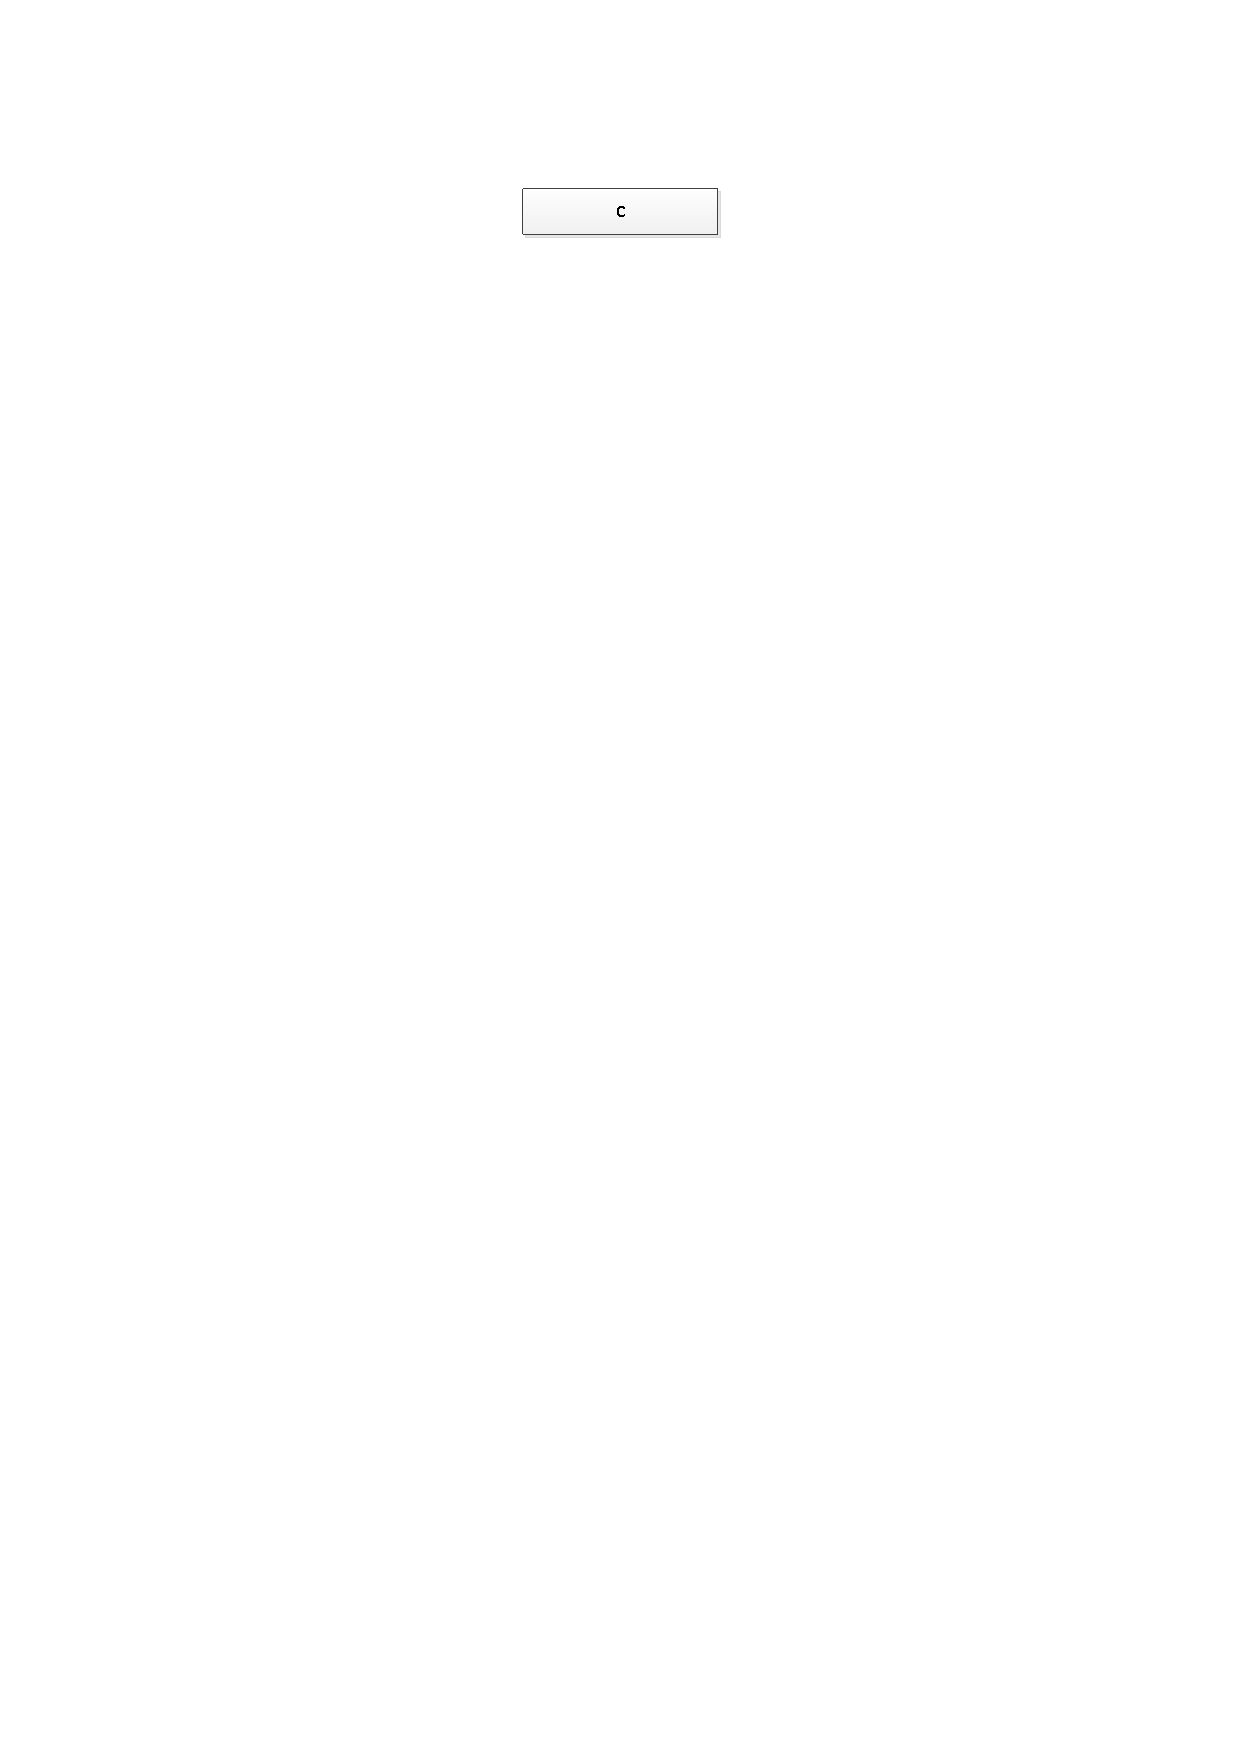
\includegraphics[trim = 85mm 257mm 70mm 22mm, clip, scale=0.75]{./diagrams/chapter5/Class}
       Class \texttt{C}       
       \vspace{2mm}
    \end{minipage}
    &
    \begin{minipage}{\dltablespacing}
       $\begin{aligned}  
       \\
	  C
         \end{aligned}$       
    \end{minipage}
    &
      $\begin{aligned}
	  &\texttt{}\\
	  &\texttt{Class: C}
     \end{aligned}$
    &
    \ref{sec_Classes} \linebreak p. \pageref{sec_Classes}\\[1mm]
    \hline
    \begin{minipage}{\umltablespacing}  
      \centering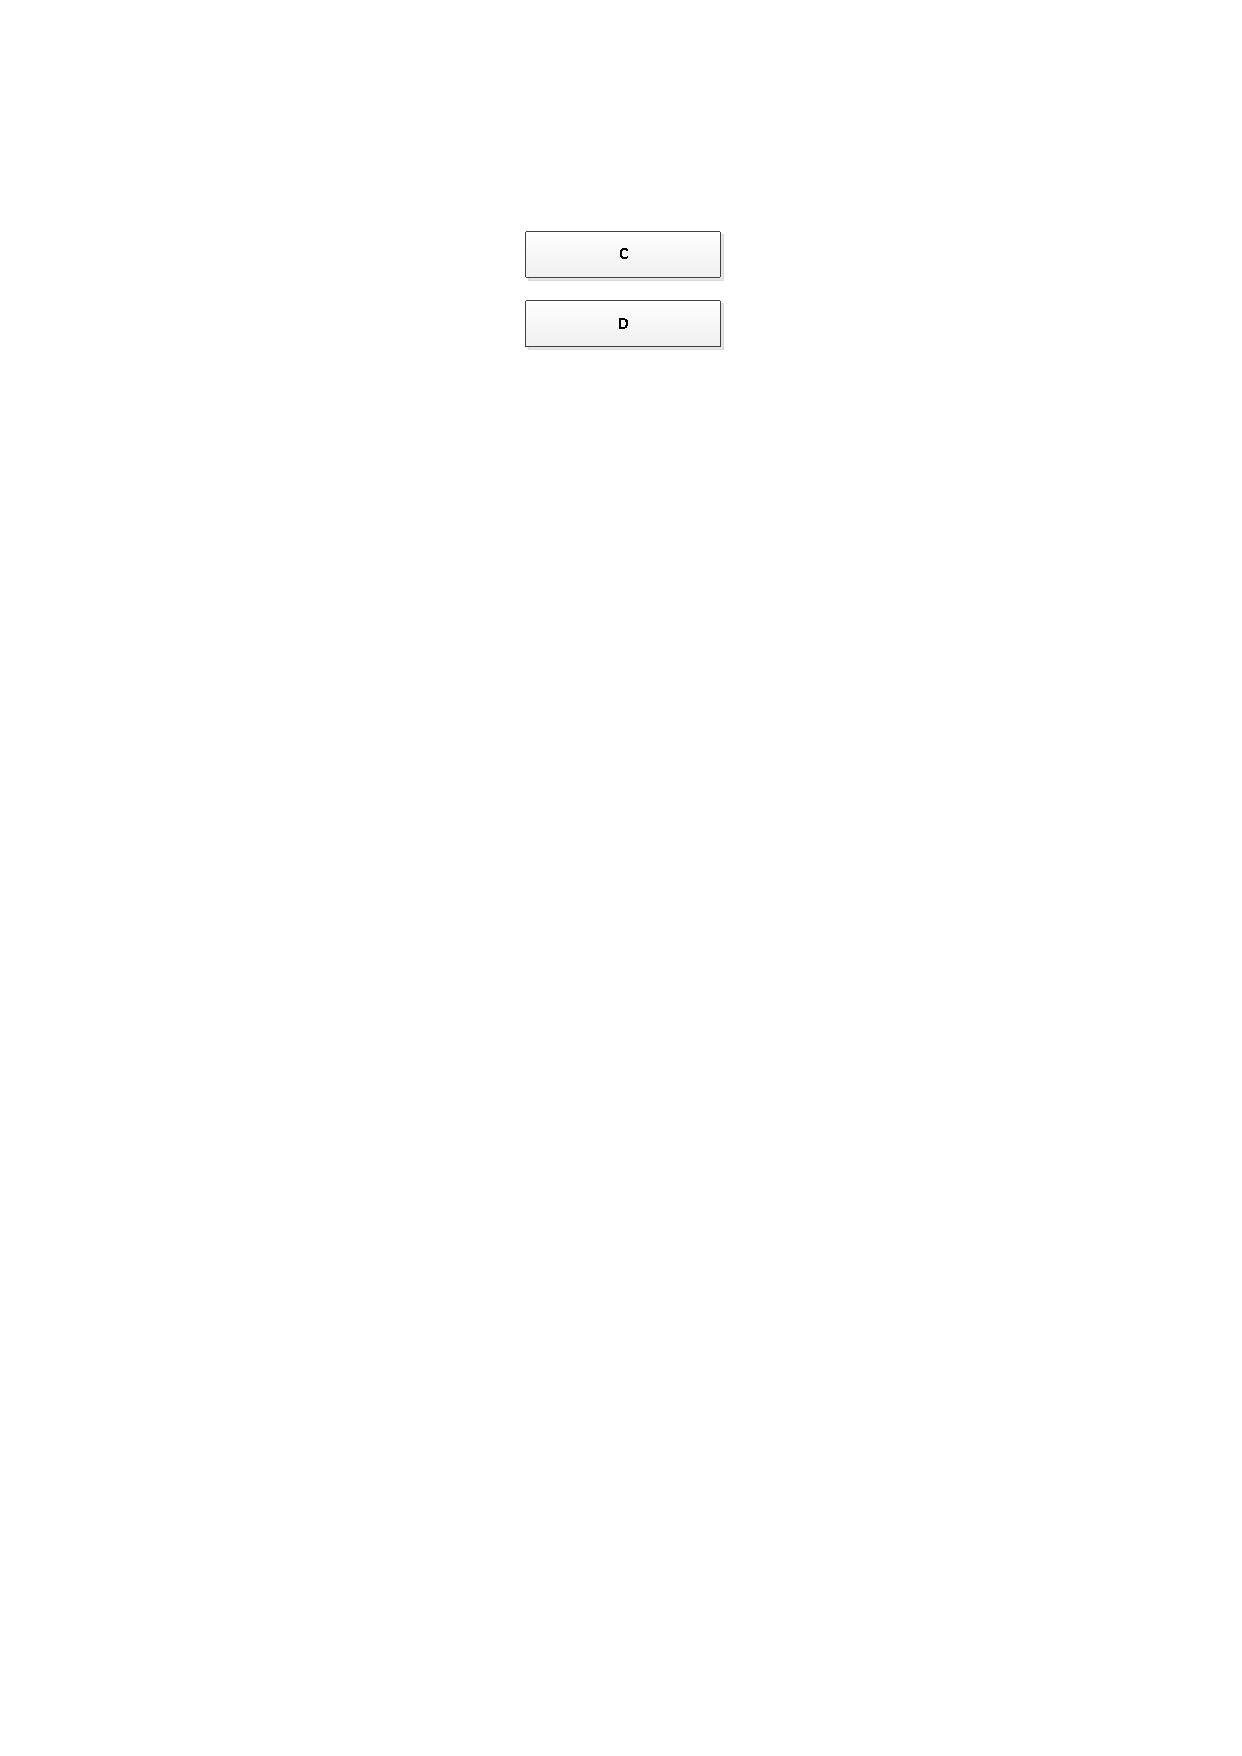
\includegraphics[trim = 85mm 238mm 70mm 28mm, clip, scale=0.75]{./diagrams/chapter5/DisjointClasses}
     Classes \texttt{C} and \texttt{D}
     \vspace{2mm}
    \end{minipage}
    &
    \begin{minipage}{\dltablespacing}
       $\begin{aligned}   
	  C \sqsubseteq \neg D
       \end{aligned}$       
    \end{minipage}
    &
      $\begin{aligned}
	  &\texttt{}\\
	  &\texttt{Class: C}\\[\owlspacing]
	  &\texttt{Class: D}\\[\owlspacing]
	  &\texttt{\hspace*{0.2cm}DisjointWith: C}
     \end{aligned}$
    &
    \ref{sec_Classes} \linebreak p. \pageref{sec_Classes}\\[5mm]
    \hline
    \begin{minipage}{\umltablespacing}    
      \centering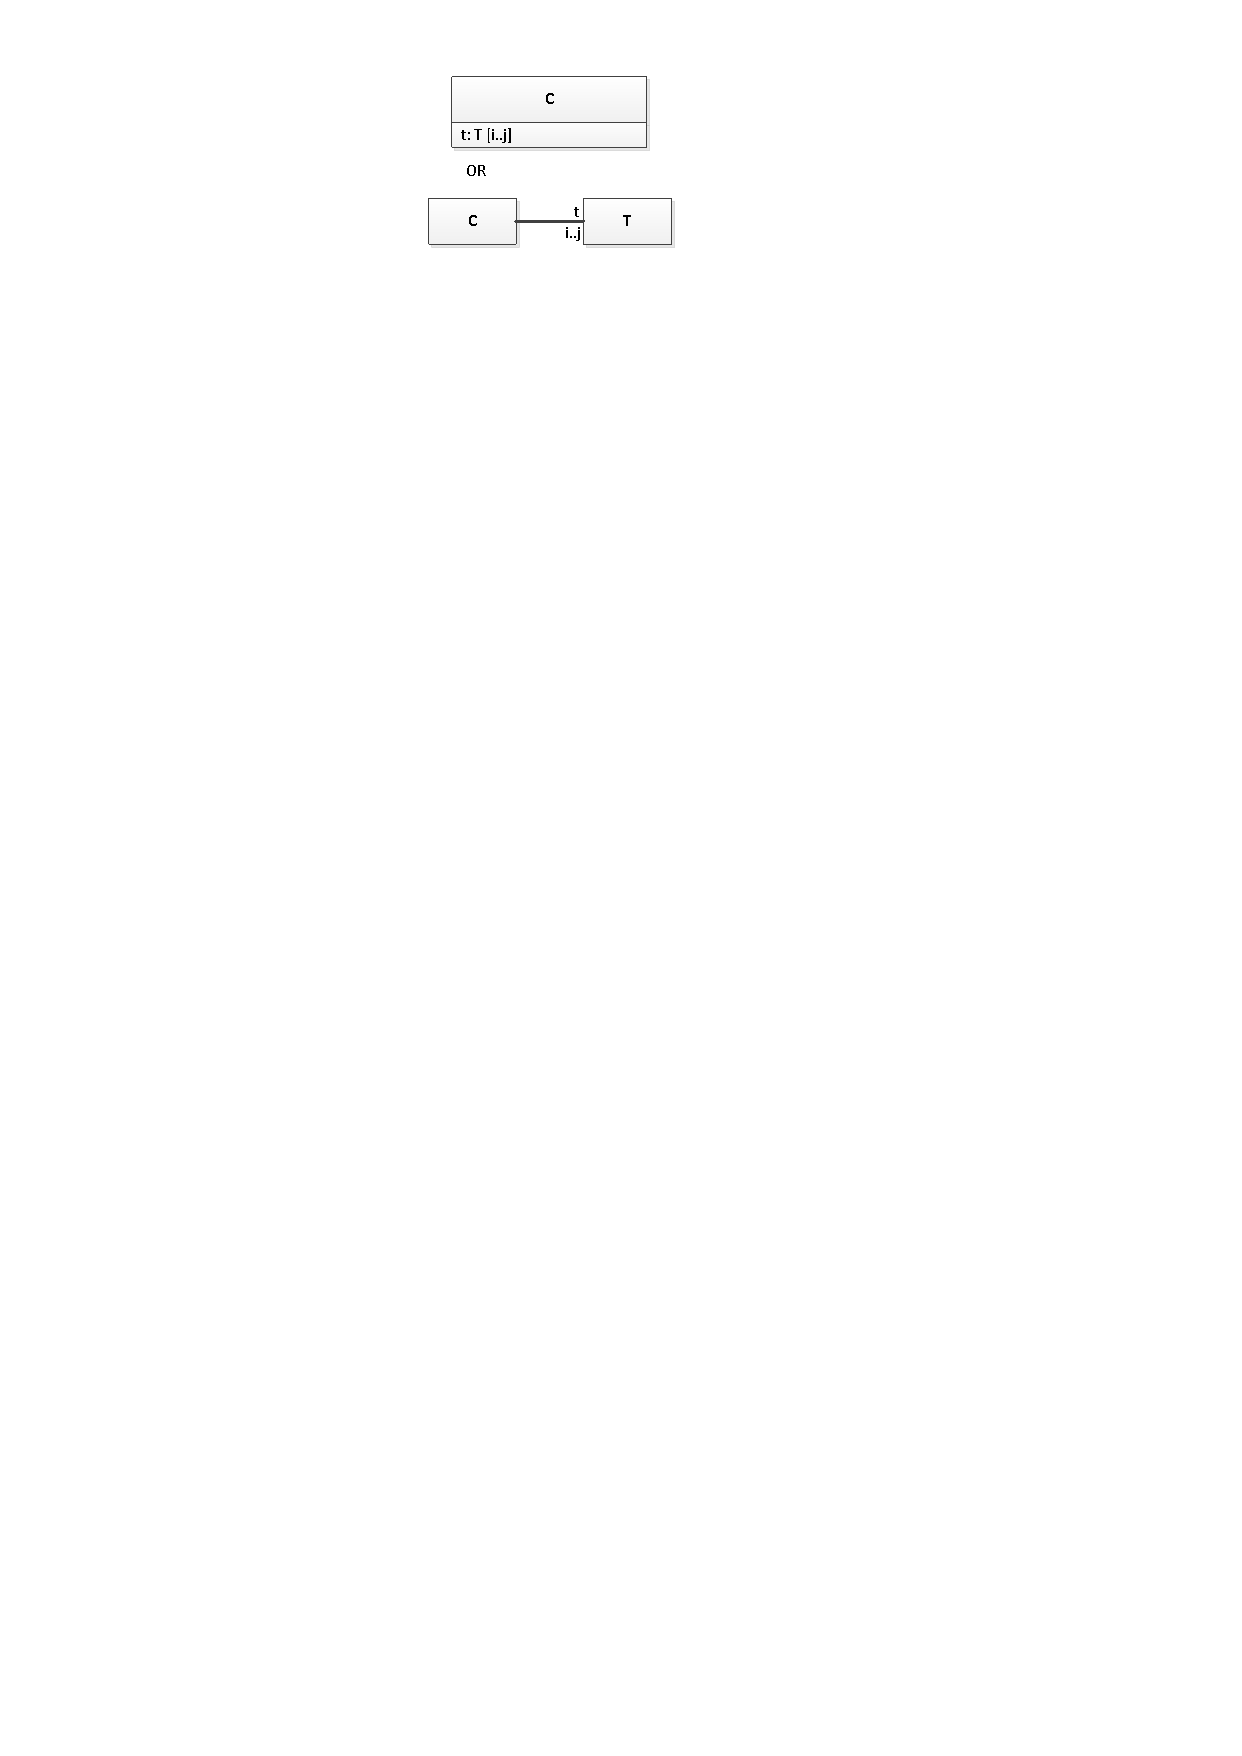
\includegraphics[trim = 72mm 250mm 92mm 4mm, clip, scale=0.75]{./diagrams/chapter5/Attribute} 
     Attribute \texttt{t} of type \texttt{T} with multiplicity \texttt{[i..j]} \\OR\\ Association end \texttt{t} of type \texttt{T} with multiplicity \texttt{[i..j]}
     \vspace{2mm}
    \end{minipage}
    &
    \begin{minipage}{\dltablespacing}
       $\begin{aligned}
	  &\exists t.\top \sqsubseteq \hspace*{2pt} C \\
          &\exists t^-.\top \sqsubseteq \hspace*{2pt} T \\
	  &C \sqsubseteq \hspace*{2pt} (\geq i \hspace*{2pt} t.\top) \hspace*{2pt} \sqcap \hspace*{2pt} (\leq j \hspace*{2pt} t.\top)
       \end{aligned}$      
    \end{minipage}
    &
      $\begin{aligned}
         &\texttt{}\\
	 &\texttt{Class: C}\\[\owlspacing]
	 &\texttt{\hspace*{2mm}SubClassOf:} \\[\owlspacing]
	 &\texttt{\hspace*{2mm}(t min i Thing) and}\\[\owlspacing]
	 &\texttt{\hspace*{4mm}(t max j Thing)} \\[\owlspacing]         
         &\texttt{Class: T}\\[\owlspacing]
         &\texttt{ObjectProperty: t} \\[\owlspacing]
         &\texttt{\hspace*{2mm}Domain: C} \\[\owlspacing]
         &\texttt{\hspace*{2mm}Range: T} \\[\owlspacing]
	 &\texttt{}\\
     \end{aligned}$
    &
    \ref{sec_Multiplicity_Attribute} \linebreak p. \pageref{sec_Multiplicity_Attribute}, \linebreak \ref{sec_attributes_sroiq} \linebreak p. \pageref{sec_attributes_sroiq} \linebreak and \linebreak 
    \ref{sec_On the Equivalence of Attributes and Binary Associations}
    \linebreak p. \pageref{sec_On the Equivalence of Attributes and Binary Associations}\\
    \hline
    \begin{minipage}{\umltablespacing}    
      \centering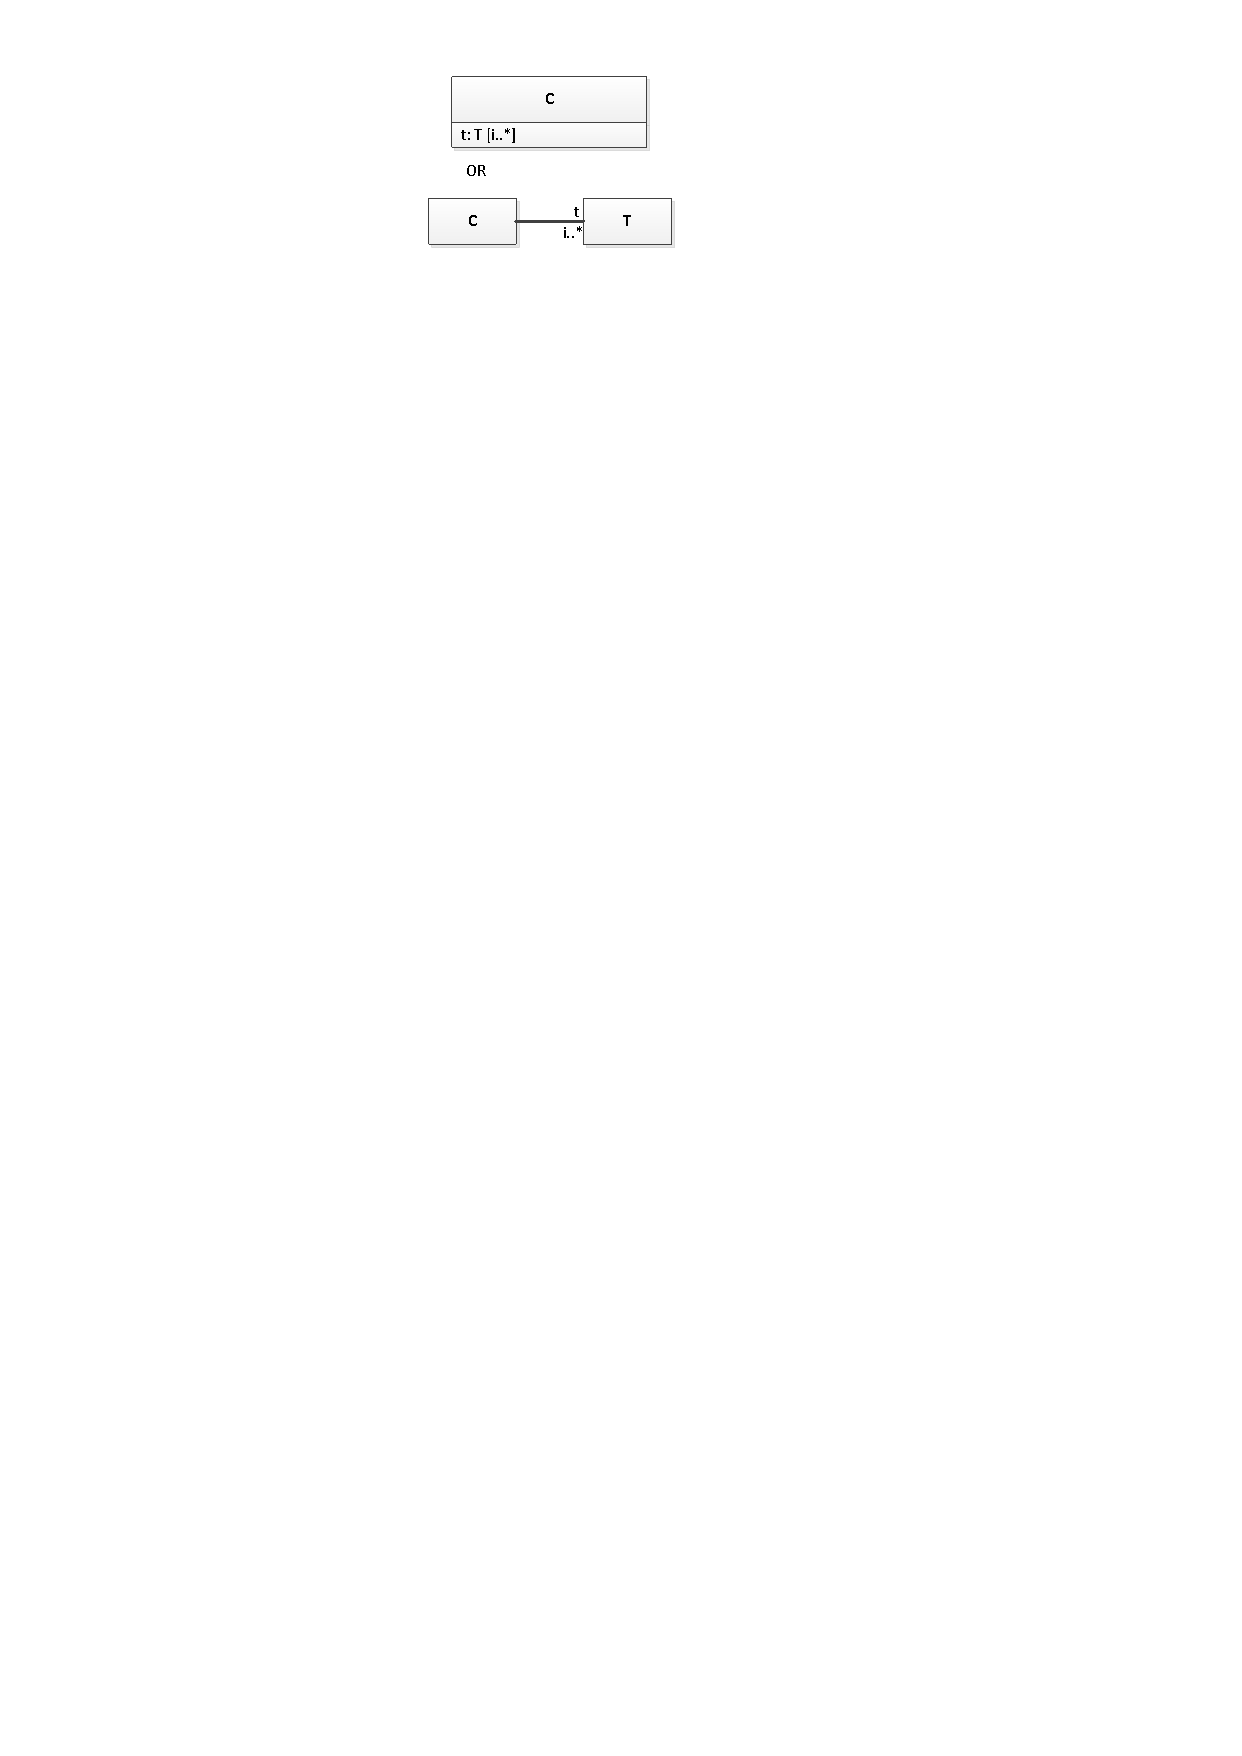
\includegraphics[trim = 72mm 250mm 92mm 4mm, clip, scale=0.75]{./diagrams/chapter5/AttributeMultiplicity_j2infinity} 
     Attribute \texttt{t} of type \texttt{T} with multiplicity \texttt{[i..*]} \\OR\\ Association end \texttt{t} of type \texttt{T} with multiplicity \texttt{[i..*]}
     \vspace{2mm}
    \end{minipage}
    &
    \begin{minipage}{\dltablespacing}
       $\begin{aligned}
	  &\exists t.\top \sqsubseteq \hspace*{2pt} C \\
          &\exists t^-.\top \sqsubseteq \hspace*{2pt} T \\
	  &C \sqsubseteq \hspace*{2pt} (\geq i \hspace*{2pt} t.\top) \hspace*{2pt}
       \end{aligned}$      
    \end{minipage}
    &
      $\begin{aligned}
         &\texttt{}\\
	 &\texttt{Class: C}\\[\owlspacing]
	 &\texttt{\hspace*{2mm}SubClassOf:} \\[\owlspacing]
	 &\texttt{\hspace*{2mm}(t min i Thing)}\\[\owlspacing]         
         &\texttt{Class: T}\\[\owlspacing]
         &\texttt{ObjectProperty: t} \\[\owlspacing]
         &\texttt{\hspace*{2mm}Domain: C} \\[\owlspacing]
         &\texttt{\hspace*{2mm}Range: T} \\[\owlspacing]
	 &\texttt{}\\
     \end{aligned}$
    &
    \ref{sec_Multiplicity_Attribute} \linebreak p. \pageref{sec_Multiplicity_Attribute}, \linebreak \ref{sec_attributes_sroiq} \linebreak p. \pageref{sec_attributes_sroiq} \linebreak and \linebreak 
    \ref{sec_On the Equivalence of Attributes and Binary Associations} \linebreak
    p. \pageref{sec_On the Equivalence of Attributes and Binary Associations}\\   
    \hline
    \begin{minipage}{\umltablespacing}    
      \centering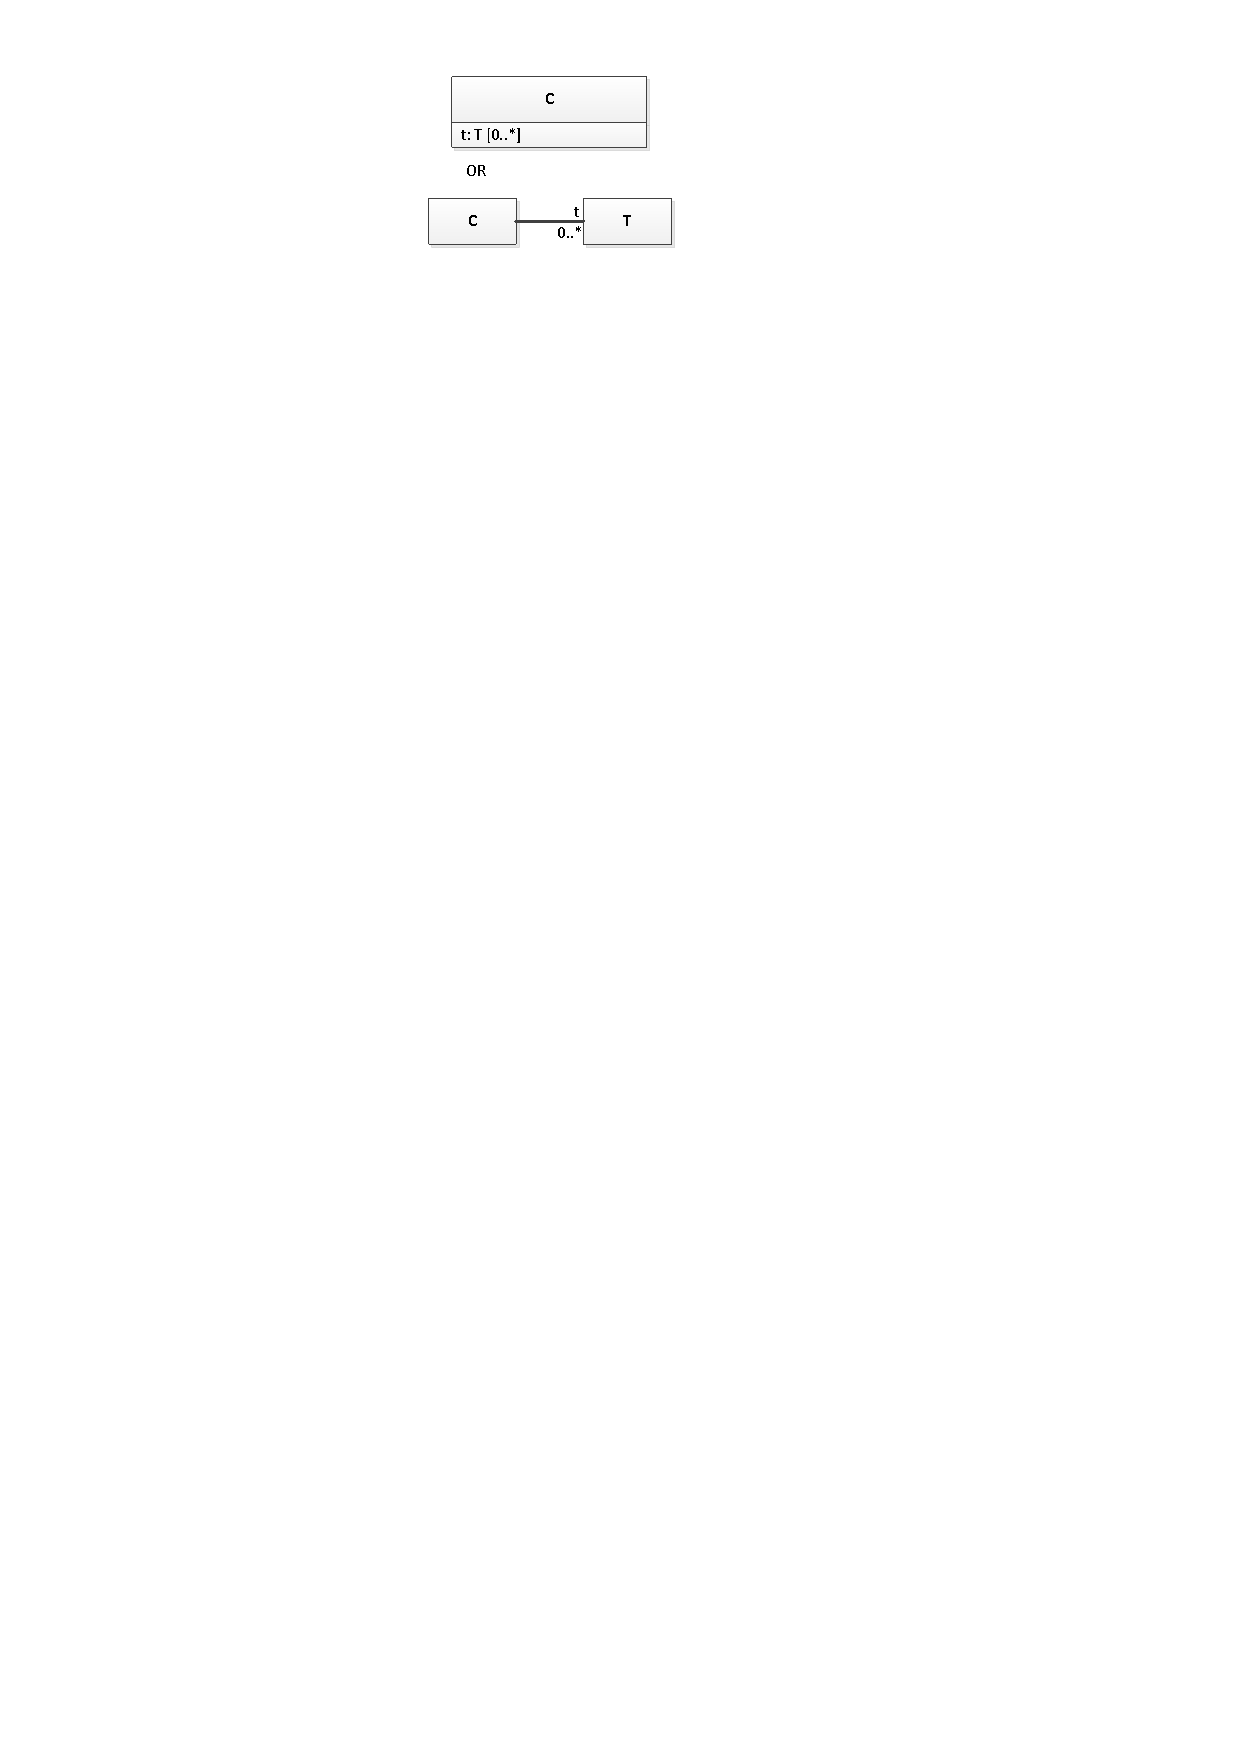
\includegraphics[trim = 72mm 250mm 92mm 4mm, clip, scale=0.75]{./diagrams/chapter5/AttributeMultiplicity_02infinity} 
     Attribute \texttt{t} of type \texttt{T} with multiplicity \texttt{[0..*]} \\OR\\ Association end \texttt{t} of type \texttt{T} with multiplicity \texttt{[0..*]}
     \vspace{2mm}
    \end{minipage}
    &
    \begin{minipage}{\dltablespacing}
       $\begin{aligned}
	  &\exists t.\top \sqsubseteq \hspace*{2pt} C \\
          &\exists t^-.\top \sqsubseteq \hspace*{2pt} T
       \end{aligned}$      
    \end{minipage}
    &
       $\begin{aligned}
         &\texttt{}\\
         &\texttt{Class: C}\\[\owlspacing]
         &\texttt{Class: T}\\[\owlspacing]
         &\texttt{ObjectProperty: t} \\[\owlspacing]
         &\texttt{\hspace*{2mm}Domain: C} \\[\owlspacing]
         &\texttt{\hspace*{2mm}Range: T} \\[\owlspacing]
	 &\texttt{}\\
     \end{aligned}$
    &
    \ref{sec_Multiplicity_Attribute} \linebreak p. \pageref{sec_Multiplicity_Attribute}, \linebreak \ref{sec_attributes_sroiq} \linebreak p. \pageref{sec_attributes_sroiq} \linebreak and \linebreak
    \ref{sec_On the Equivalence of Attributes and Binary Associations} \linebreak
    p. \pageref{sec_On the Equivalence of Attributes and Binary Associations}\\  
    \hline
    \begin{minipage}{\umltablespacing}    
      \centering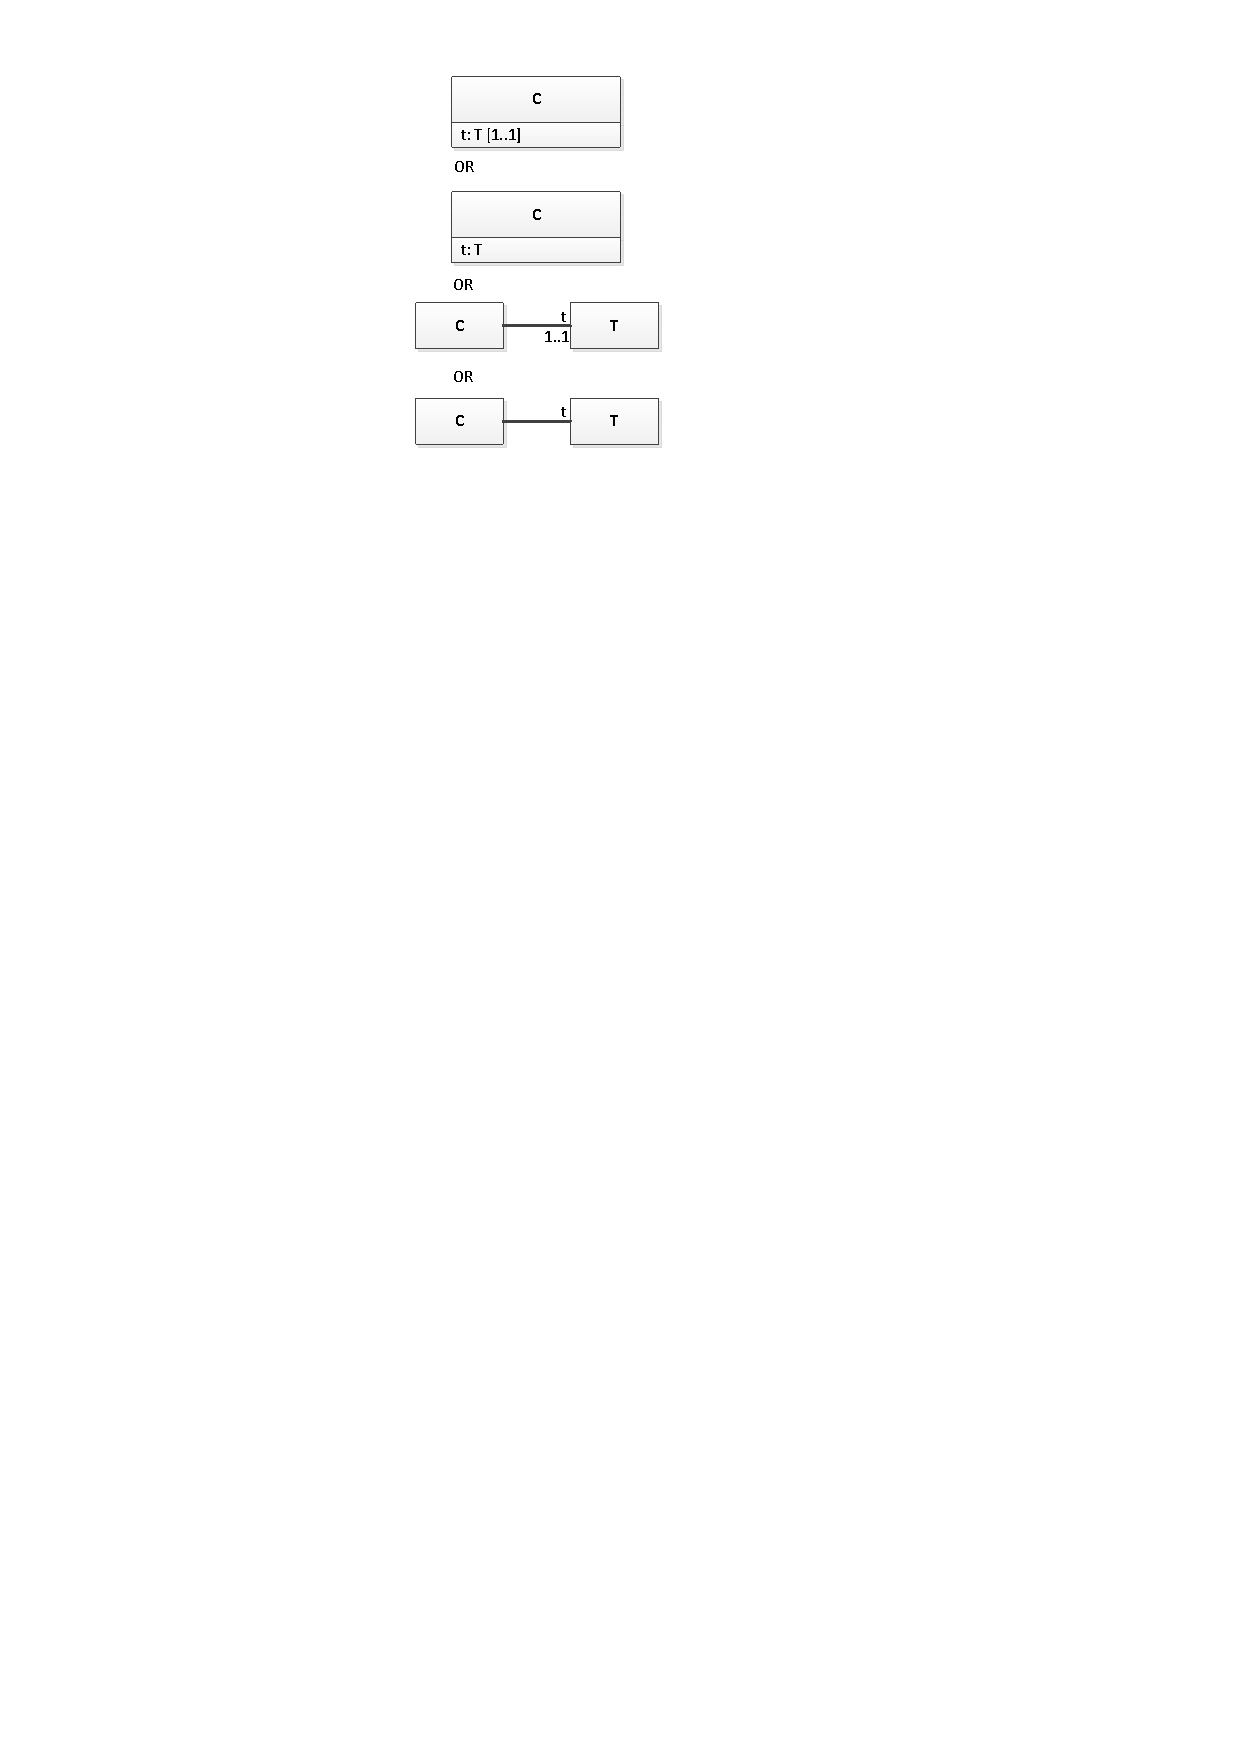
\includegraphics[trim = 70mm 220mm 92mm 4mm, clip, scale=0.75]{./diagrams/chapter5/AttributeMultiplicity1} 
     Attribute \texttt{t} of type \texttt{T} with multiplicity \texttt{[1..1]} \\OR\\ Association end \texttt{t} of type \texttt{T} with multiplicity \texttt{[1..1]}
     \vspace{2mm}
    \end{minipage}
    &
    \begin{minipage}{\dltablespacing}
       $\begin{aligned}
       	 &\exists t.\top \sqsubseteq \hspace*{2pt} C \\
         &\exists t^-.\top \sqsubseteq \hspace*{2pt} T \\
	 &C \sqsubseteq \exists t.\top \sqcap (\leq 1 \hspace*{2pt} t. \top)
       \end{aligned}$      
    \end{minipage}
    &
      $\begin{aligned}
	&\texttt{Class: C}\\[\owlspacing]
   	&\texttt{\hspace*{2mm}SubClassOf:}\\[\owlspacing]
   	&\texttt{\hspace*{4mm}t exactly 1 Thing}\\[\owlspacing]      
	&\texttt{Class: T}
     \end{aligned}$
    &
%    \ref{sec_Multiplicity_Attribute} \linebreak p. \pageref{sec_Multiplicity_Attribute} \linebreak and \linebreak \ref{sec_attributes_sroiq} \linebreak p. \pageref{sec_attributes_sroiq} \\    
    \ref{sec_Multiplicity_Attribute} \linebreak p. \pageref{sec_Multiplicity_Attribute}, \linebreak \ref{sec_attributes_sroiq} \linebreak p. \pageref{sec_attributes_sroiq} \linebreak and \linebreak
    \ref{sec_On the Equivalence of Attributes and Binary Associations} \linebreak
    p. \pageref{sec_On the Equivalence of Attributes and Binary Associations}\\
    \hline    
    \begin{minipage}{\umltablespacing}    
      \centering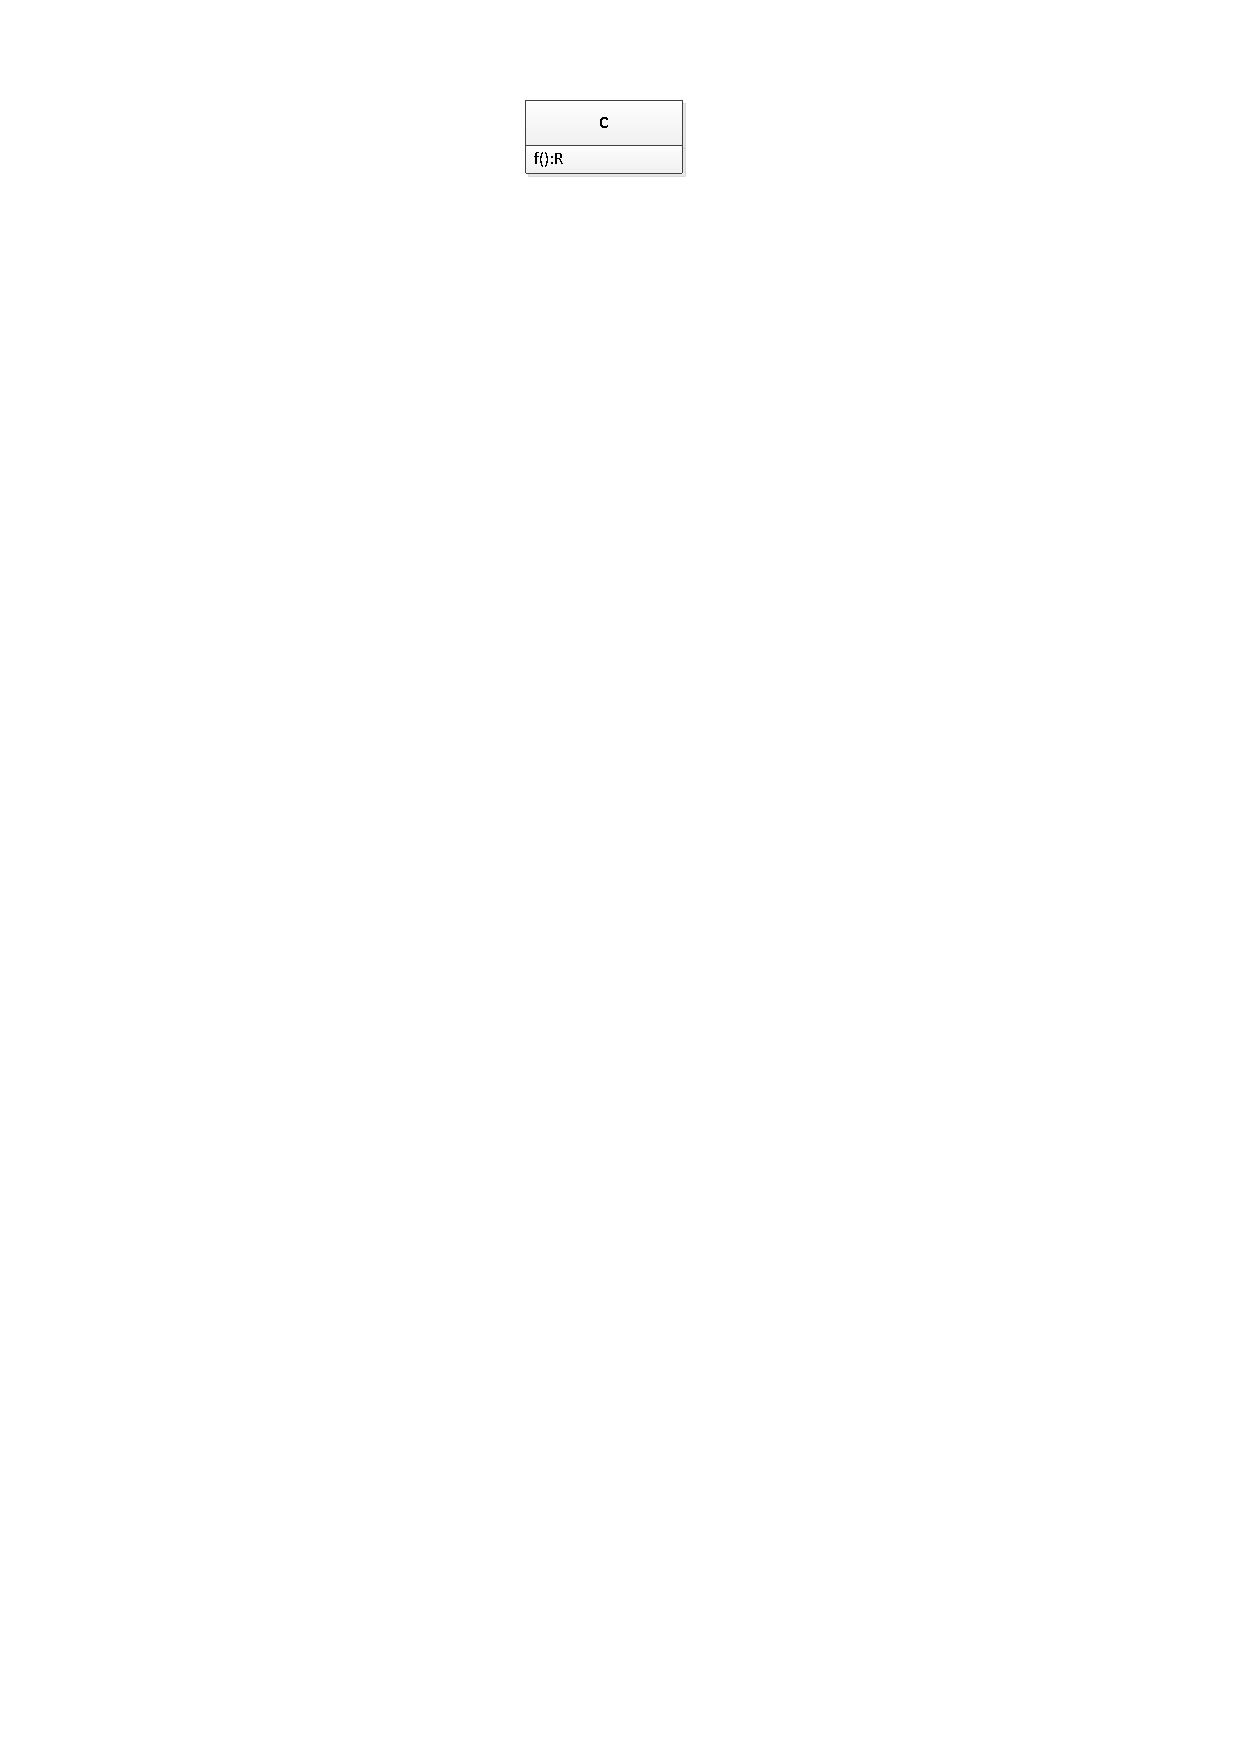
\includegraphics[trim = 82mm 265mm 88mm 4mm, clip, scale=0.75]{./diagrams/chapter5/OperationNoParameters} 
     Operation \texttt{f} with no parameters returning a value of type \texttt{R}
    % \vspace{2mm}
    \end{minipage}
    &
    \begin{minipage}{\dltablespacing}
       $\begin{aligned}
       \\
	&C_{f():R} \sqsubseteq \hspace*{1mm} \exists f^-.\top \sqcap (\leq 1 f^-.\top) \hspace*{1mm} \sqcap \\
  	&\hspace*{1mm} \exists r_R.\top \sqcap (\leq 1 r_R.\top)\\
  	\\
	&\exists f^-.\top \sqsubseteq C_{f():R}\\
	&\exists f.\top \sqsubseteq C \\
	&\exists r_R.\top \sqsubseteq C_{f():R}\\
	&\exists r_R^-.\top \sqsubseteq R\\
	\\
	&C \sqsubseteq \exists f. C_{f():R}\\
	\\
       \end{aligned}$      
       Note that determinism of the return value cannot be enforced since rule-like constructs are required which are not supported in $\mathcal{SROIQ}^{(\mathcal{D})}$\\
    \end{minipage}
    &
     $\begin{aligned}
     \\
  	&\texttt{Class: C\_f()\_R} \\[\owlspacing]
  	&\texttt{\hspace*{2mm}SubClassOf:}\\[\owlspacing]
  	&\texttt{\hspace*{4mm}f\_inv exactly 1 Thing}\\[\owlspacing]
  	&\texttt{\hspace*{4mm}and}\\[\owlspacing]
  	&\texttt{\hspace*{4mm}r\_R exactly 1 Thing}\\[\owlspacing]
  	&\texttt{\hspace*{2mm}Haskey: f\_inv} \\
  	 &\texttt{ObjectProperty: f\_inv}\\[\owlspacing]
         &\texttt{\hspace*{2mm}Domain: C\_f()\_R}\\[\owlspacing]
         &\texttt{\hspace*{2mm}Range: C}\\[\owlspacing]
         &\texttt{ObjectProperty: f}\\[\owlspacing]
         &\texttt{\hspace*{2mm}InverseOf: f\_inv}\\[\owlspacing]
         &\texttt{ObjectProperty: r\_R}\\[\owlspacing]
         &\texttt{\hspace*{2mm}Domain: C\_f()\_R}\\[\owlspacing]
         &\texttt{\hspace*{2mm}Range: R}\\
         &\texttt{Class: C}\\[\owlspacing]
         &\texttt{\hspace*{2mm}SubClassOf:}\\[\owlspacing]
         &\texttt{\hspace*{4mm}f some C\_f()\_R}\\
         &\texttt{Class: R}\\[\owlspacing]   
         \\
     \end{aligned}$
    &
    \ref{sec_operations_sroiq} \linebreak p. \pageref{sec_operations_sroiq} \linebreak and \linebreak \ref{sec_Operations Revisited} \linebreak p. \pageref{sec_Operations Revisited} \\    
    \hline    
    \begin{minipage}{\umltablespacing}    
      \centering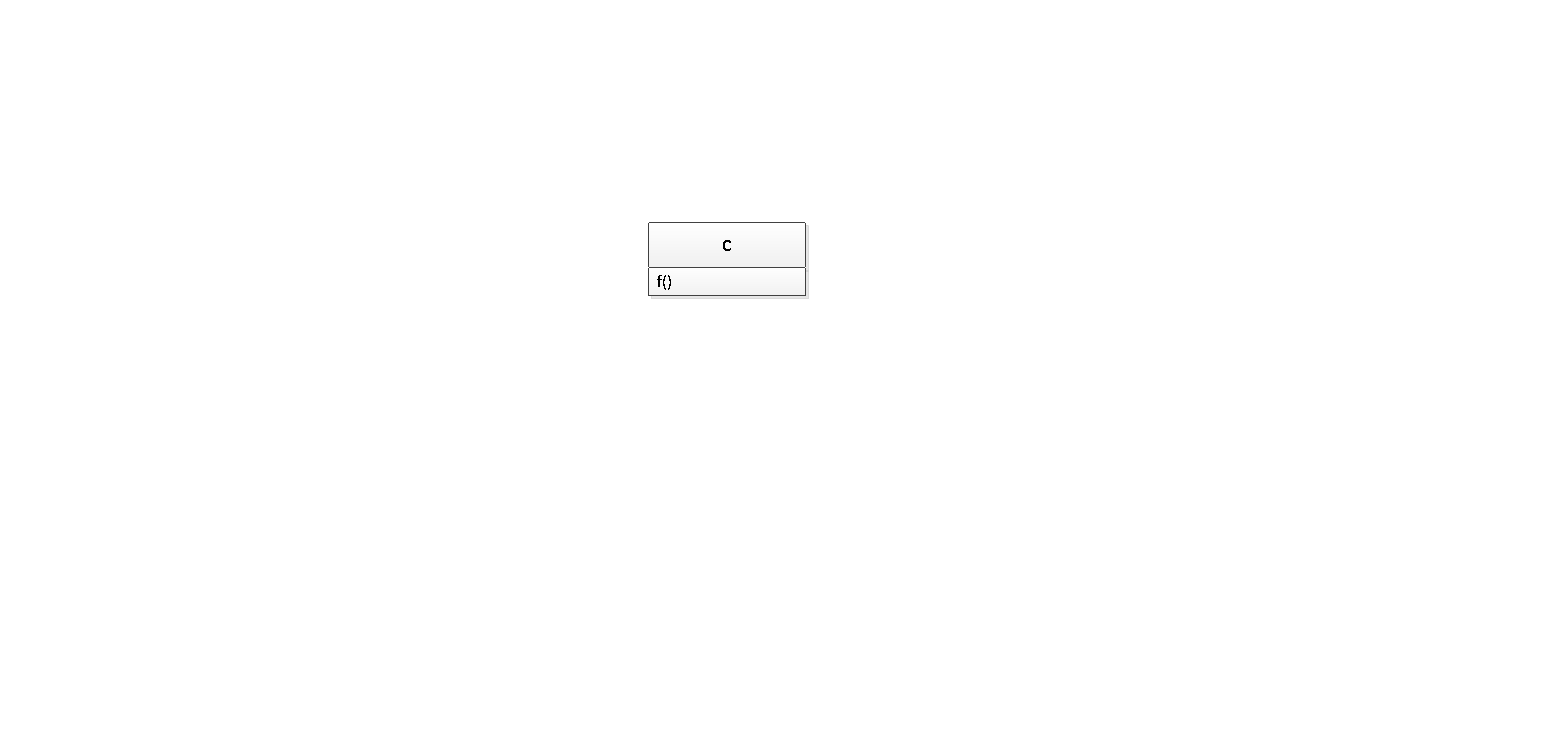
\includegraphics[trim = 103mm 70mm 8mm 24mm, clip, scale=0.75]{./diagrams/chapter5/OperationNoParametersNoReturn} 
     Operation \texttt{f} with no parameters and no return value
    % \vspace{2mm}
    \end{minipage}
    &
    \begin{minipage}{\dltablespacing}
       $\begin{aligned}
       \\
	&C_{f()} \sqsubseteq \hspace*{1mm} \exists f^-.\top \sqcap (\leq 1 f^-.\top) \hspace*{1mm}\\ 
  	\\
	&\exists f^-.\top \sqsubseteq C_{f()}\\
	&\exists f.\top \sqsubseteq C \\
	\\
	&C \sqsubseteq \exists f. C_{f()}\\
	\\
       \end{aligned}$      
    \end{minipage}
    &
     $\begin{aligned}
     \\
  	&\texttt{Class: C\_f()} \\[\owlspacing]
  	&\texttt{\hspace*{2mm}SubClassOf:}\\[\owlspacing]
  	&\texttt{\hspace*{4mm}f\_inv exactly 1 Thing}\\[\owlspacing]
  	 &\texttt{ObjectProperty: f\_inv}\\[\owlspacing]
         &\texttt{\hspace*{2mm}Domain: C\_f()}\\[\owlspacing]
         &\texttt{\hspace*{2mm}Range: C}\\[\owlspacing]
         &\texttt{ObjectProperty: f}\\[\owlspacing]
         &\texttt{\hspace*{2mm}InverseOf: f\_inv}\\[\owlspacing]
         &\texttt{Class: C}\\[\owlspacing]
         &\texttt{\hspace*{2mm}SubClassOf:}\\[\owlspacing]
         &\texttt{\hspace*{4mm}f some C\_f()}\\  
         \\
     \end{aligned}$
    &
    \ref{sec_operations_sroiq} \linebreak p. \pageref{sec_operations_sroiq} \linebreak and \linebreak \ref{sec_Operations Revisited} \linebreak p. \pageref{sec_Operations Revisited} \\       
    \hline        
    \begin{minipage}{\umltablespacing}    
      \centering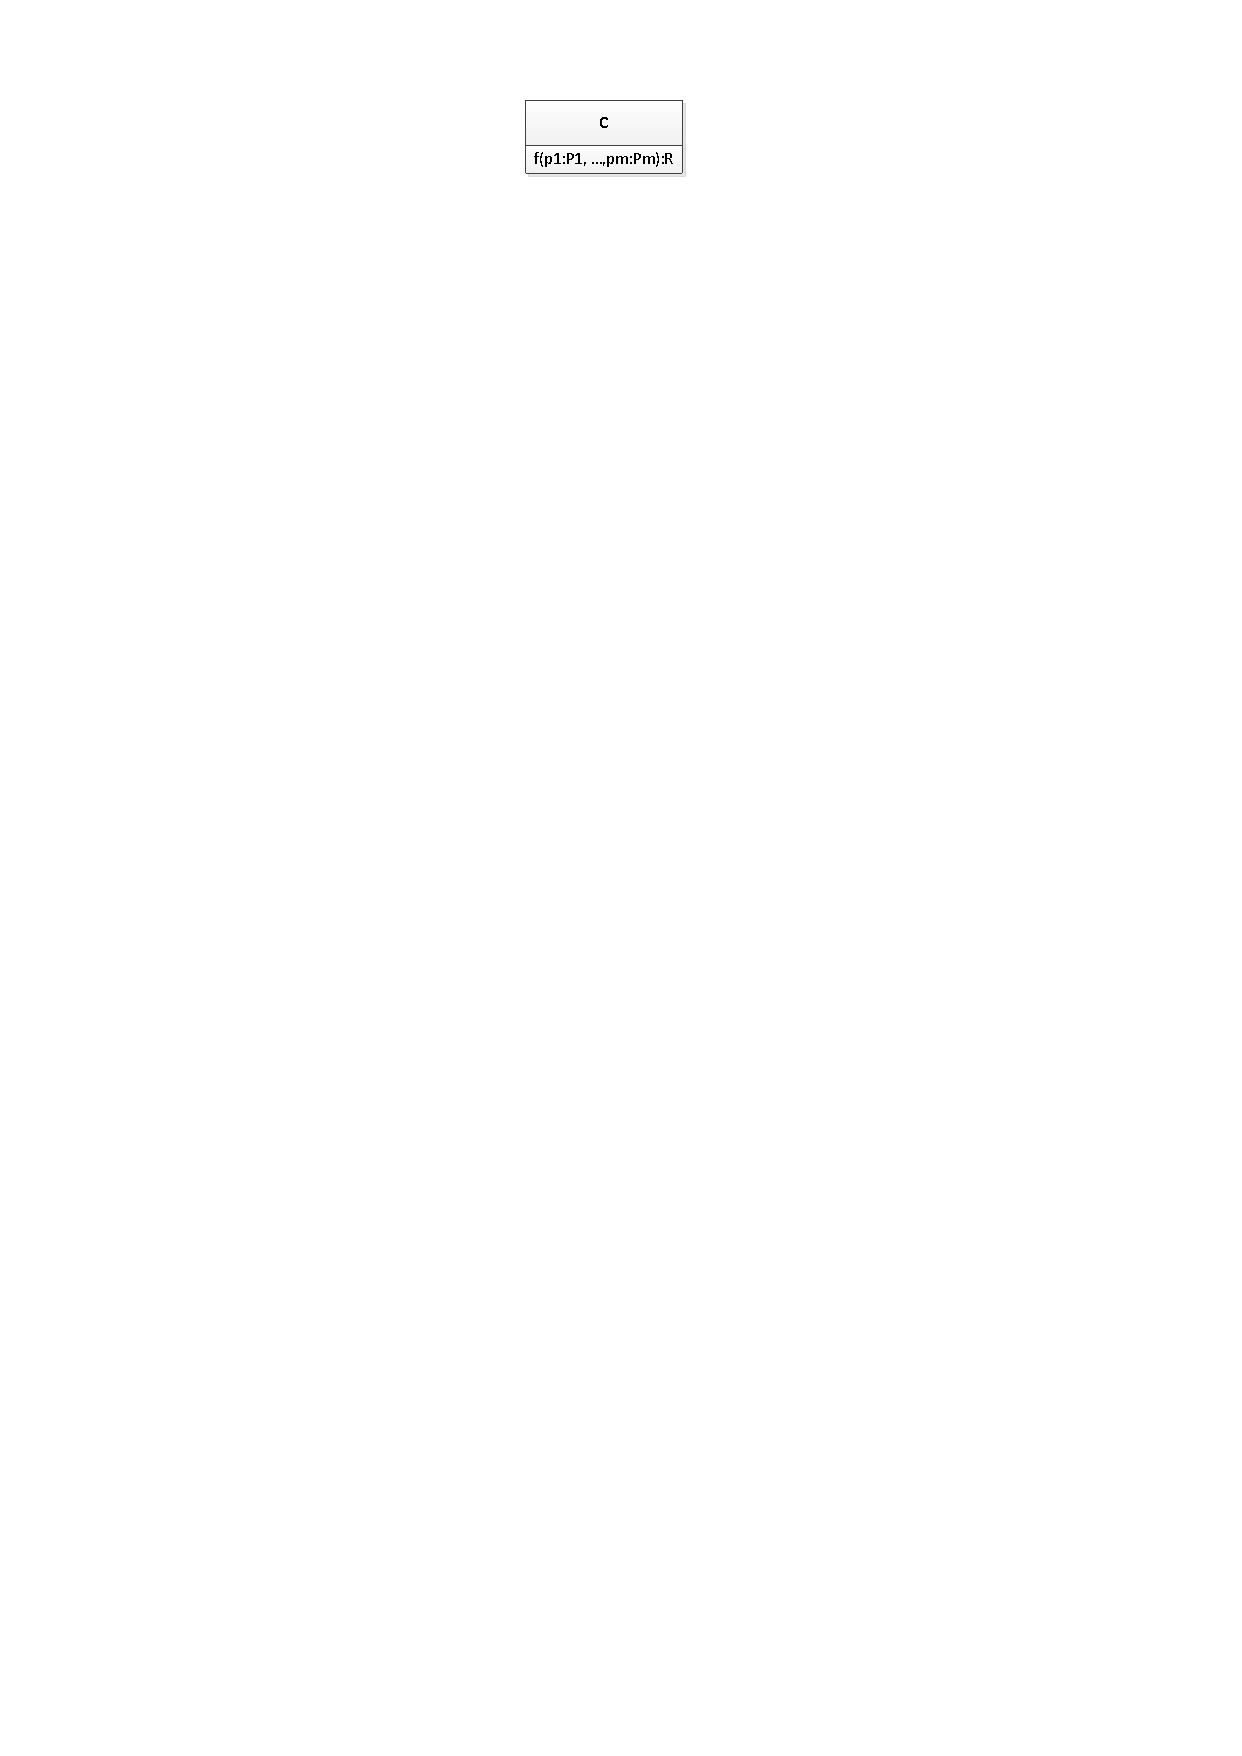
\includegraphics[trim = 82mm 265mm 88mm 4mm, clip, scale=0.75]{./diagrams/chapter5/Operation} 
     Operation \texttt{f} with parameters \texttt{p1, ...,pm} respectively of type \texttt{P1, ..., Pm} returning a value of type \texttt{R}
     \vspace{2mm}
    \end{minipage}
    &
    \begin{minipage}{\dltablespacing}
       $\begin{aligned}
\\
  	&C_{f(P_1, ..., P_m):R} \sqsubseteq\\
  	\hspace*{1mm}& \exists f^-.\top \sqcap (\leq 1 f^-.\top) \hspace*{1mm} \sqcap \\
  	 \hspace*{1mm}& \exists p_1.\top \sqcap (\leq 1 p_1.\top) \hspace*{1mm} \sqcap \\
  	\hspace*{1mm}& \vdots  \\
  	\hspace*{1mm}& \exists p_m.\top \sqcap (\leq 1 p_m.\top) \hspace*{1mm} \sqcap \\
  	\hspace*{1mm}& \exists r_R.\top \sqcap (\leq 1 r_R.\top)\\
       \\
       &\exists p_i.\top \sqsubseteq C_{f(P_1, ..., P_m):R}\\
       &\exists p_i^-.\top \sqsubseteq P_i \hspace*{5mm} i = 1, \ldots, m \\
       \\
       &\exists f^-.\top \sqsubseteq C_{f(P_1, ..., P_m):R} \\
       &\exists f.\top \sqsubseteq C \\
       &\exists r_R.\top \sqsubseteq C_{f(P_1, ..., P_m):R}\\ 
       &\exists r_R^-.\top \sqsubseteq R\\
	\\
	&C \sqsubseteq \exists f. C_{f(P_1, \ldots, P_m):R}\\
	\\
       \end{aligned}$  
       Note that determinism of the return value cannot be enforced since rule-like constructs are required which are not supported in $\mathcal{SROIQ}^{(\mathcal{D})}$
    \end{minipage}
     &
     $\begin{aligned}
     \\
	&\texttt{Class: P1}\\[\owlspacing]
	&\texttt{\hspace*{4mm}}\vdots \\[\owlspacing]
	&\texttt{Class: Pm}\\[\owlspacing]     
  	&\texttt{Class: C\_f(P1,..., Pm)\_R} \\[\owlspacing]
  	&\texttt{\hspace*{2mm}SubClassOf:}\\[\owlspacing]
  	&\texttt{\hspace*{4mm}f\_inv exactly 1 Thing}\\[\owlspacing]
  	&\texttt{\hspace*{6mm}and}\\[\owlspacing]
  	&\texttt{\hspace*{4mm}p1 exactly 1 Thing and}\\[\owlspacing]
  	&\texttt{\hspace*{6mm}} \vdots \\[\owlspacing]
  	&\texttt{\hspace*{4mm}pm exactly 1 Thing and}\\[\owlspacing]
  	&\texttt{\hspace*{4mm}r\_R exactly 1 Thing}\\[\owlspacing]
         &\texttt{\hspace*{2mm}Haskey:}\\[\owlspacing] 
         &\texttt{\hspace*{4mm}f\_inv, p1, ..., pm} \\  	
         &\texttt{ObjectProperty: p1}\\[\owlspacing]
         &\texttt{\hspace*{2mm}Domain: C\_f(P1,..., Pm)\_R}\\[\owlspacing]
         &\texttt{\hspace*{2mm}Range: P1}\\[\owlspacing]
         &\texttt{\hspace*{4mm}}\vdots \\[\owlspacing]
         &\texttt{ObjectProperty: pm}\\[\owlspacing]
         &\texttt{\hspace*{2mm}Domain: C\_f(P1,..., Pm)\_R}\\[\owlspacing]
         &\texttt{\hspace*{2mm}Range: Pm}\\
         &\texttt{ObjectProperty: f\_inv}\\[\owlspacing]
         &\texttt{\hspace*{2mm}Domain: C\_f(P1,..., Pm)\_R}\\[\owlspacing]
         &\texttt{\hspace*{2mm}Range: C}\\[\owlspacing]
         &\texttt{ObjectProperty: f}\\[\owlspacing]
         &\texttt{\hspace*{2mm}InverseOf: f\_inv}\\[\owlspacing]
         &\texttt{ObjectProperty: r\_R}\\[\owlspacing]
         &\texttt{\hspace*{2mm}Domain: C\_f(P1,..., Pm)\_R}\\[\owlspacing]
         &\texttt{\hspace*{2mm}Range: R}\\
         &\texttt{Class: C}\\[\owlspacing]
         &\texttt{\hspace*{2mm}SubClassOf: }\\[\owlspacing]
         &\texttt{\hspace*{4mm}f some C\_f(P1,..., Pm)\_R}\\
         &\texttt{Class: R}\\[\owlspacing]     
         \\
     \end{aligned}$
    &
    \ref{sec_operations_sroiq} \linebreak p. \pageref{sec_operations_sroiq} \linebreak and \ref{sec_Operations Revisited} \linebreak p. \pageref{sec_Operations Revisited}\\     
    \hline        
    \begin{minipage}{\umltablespacing}    
      \centering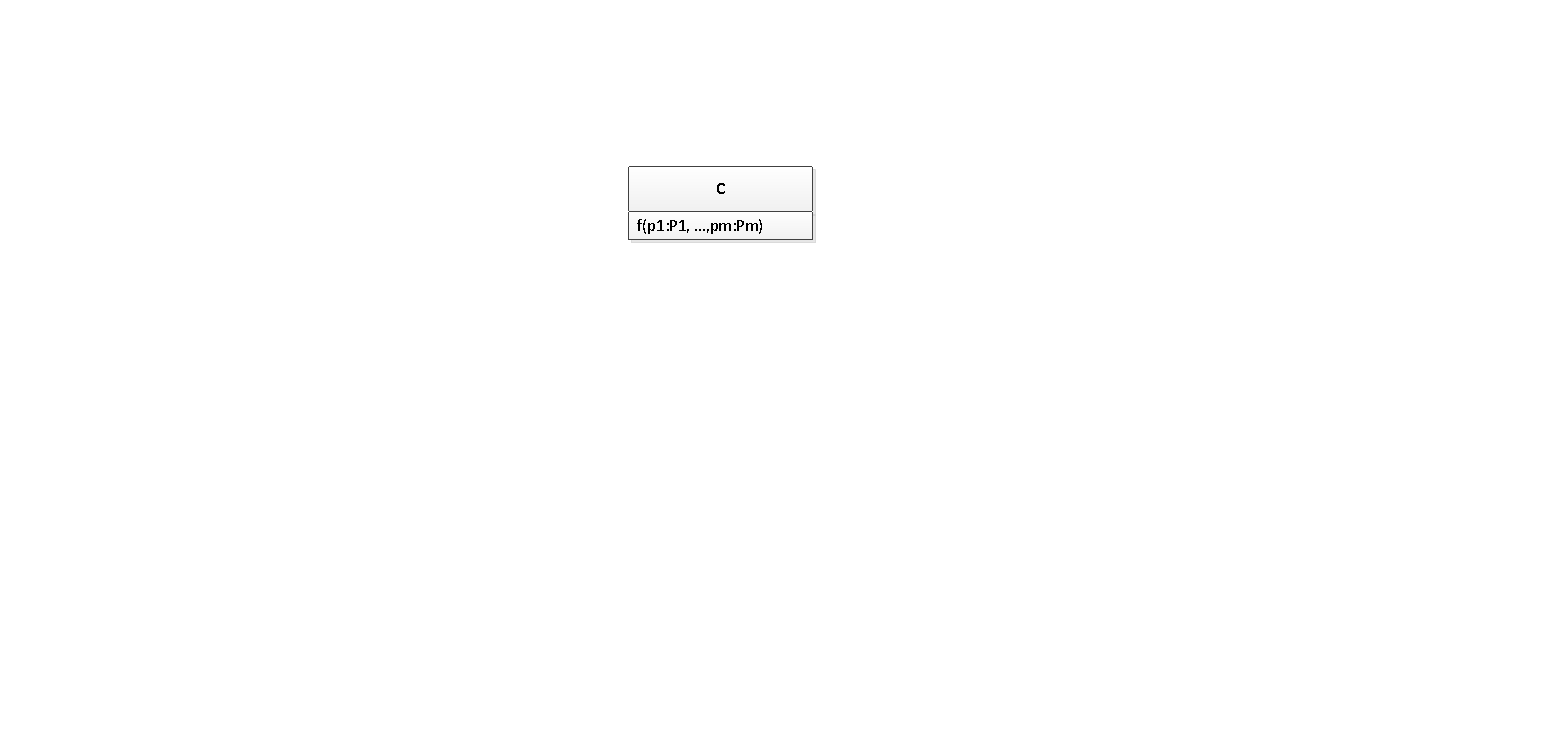
\includegraphics[trim = 102mm 80mm 88mm 24mm, clip, scale=0.75]{./diagrams/chapter5/OperationNoReturn} 
     Operation \texttt{f} with parameters \texttt{p1, ...,pm} respectively of type \texttt{P1, ..., Pm} and no return value
     \vspace{2mm}
    \end{minipage}
    &
    \begin{minipage}{\dltablespacing}
       $\begin{aligned}
\\
  	&C_{f(P_1, ..., P_m)} \sqsubseteq\\
  	\hspace*{1mm}& \exists f^-.\top \sqcap (\leq 1 f^-.\top) \hspace*{1mm} \sqcap \\
  	 \hspace*{1mm}& \exists p_1.\top \sqcap (\leq 1 p_1.\top) \hspace*{1mm} \sqcap \\
  	\hspace*{1mm}& \vdots  \\
  	\hspace*{1mm}& \exists p_m.\top \sqcap (\leq 1 p_m.\top) \hspace*{1mm} \\
       \\
       &\exists p_i.\top \sqsubseteq C_{f(P_1, ..., P_m)} \\
       &\exists p_i^-.\top \sqsubseteq P_i \hspace*{5mm} i = 1, \ldots, m \\
       \\
       &\exists f^-.\top \sqsubseteq C_{f(P_1, ..., P_m)} \\
       &\exists f.\top \sqsubseteq C \\
	\\
	&C \sqsubseteq \exists f. C_{f(P_1, \ldots, P_m)}\\
	\\
       \end{aligned}$  
    \end{minipage}
     &
     $\begin{aligned}
     \\
	&\texttt{Class: P1}\\[\owlspacing]
	&\texttt{\hspace*{4mm}}\vdots \\[\owlspacing]
	&\texttt{Class: Pm}\\[\owlspacing]          
  	&\texttt{Class: C\_f(P1,..., Pm)} \\[\owlspacing]
  	&\texttt{\hspace*{2mm}SubClassOf:}\\[\owlspacing]
  	&\texttt{\hspace*{4mm}f\_inv exactly 1 Thing}\\[\owlspacing]
  	&\texttt{\hspace*{6mm}and}\\[\owlspacing]
  	&\texttt{\hspace*{4mm}p1 exactly 1 Thing and}\\[\owlspacing]
  	&\texttt{\hspace*{6mm}} \vdots \\[\owlspacing]
  	&\texttt{\hspace*{4mm}pm exactly 1 Thing}\\[\owlspacing]
         &\texttt{ObjectProperty: p1}\\[\owlspacing]
         &\texttt{\hspace*{2mm}Domain: C\_f(P1,..., Pm)}\\[\owlspacing]
         &\texttt{\hspace*{2mm}Range: P1}\\[\owlspacing]
         &\texttt{\hspace*{4mm}}\vdots \\[\owlspacing]
         &\texttt{ObjectProperty: pm}\\[\owlspacing]
         &\texttt{\hspace*{2mm}Domain: C\_f(P1,..., Pm)}\\[\owlspacing]
         &\texttt{\hspace*{2mm}Range: Pm}\\
         &\texttt{ObjectProperty: f\_inv}\\[\owlspacing]
         &\texttt{\hspace*{2mm}Domain: C\_f(P1,..., Pm)}\\[\owlspacing]
         &\texttt{\hspace*{2mm}Range: C}\\[\owlspacing]
         &\texttt{ObjectProperty: f}\\[\owlspacing]
         &\texttt{\hspace*{2mm}InverseOf: f\_inv}\\[\owlspacing]
         &\texttt{Class: C}\\[\owlspacing]
         &\texttt{\hspace*{2mm}SubClassOf: }\\[\owlspacing]
         &\texttt{\hspace*{4mm}f some C\_f(P1,..., Pm)}\\
         \\
     \end{aligned}$
    &
    \ref{sec_operations_sroiq} \linebreak p. \pageref{sec_operations_sroiq} \linebreak and \linebreak \ref{sec_Operations Revisited} \linebreak p. \pageref{sec_Operations Revisited}\\ 
    \hline  
    \begin{minipage}{\umltablespacing}
      \centering\hspace*{-4mm}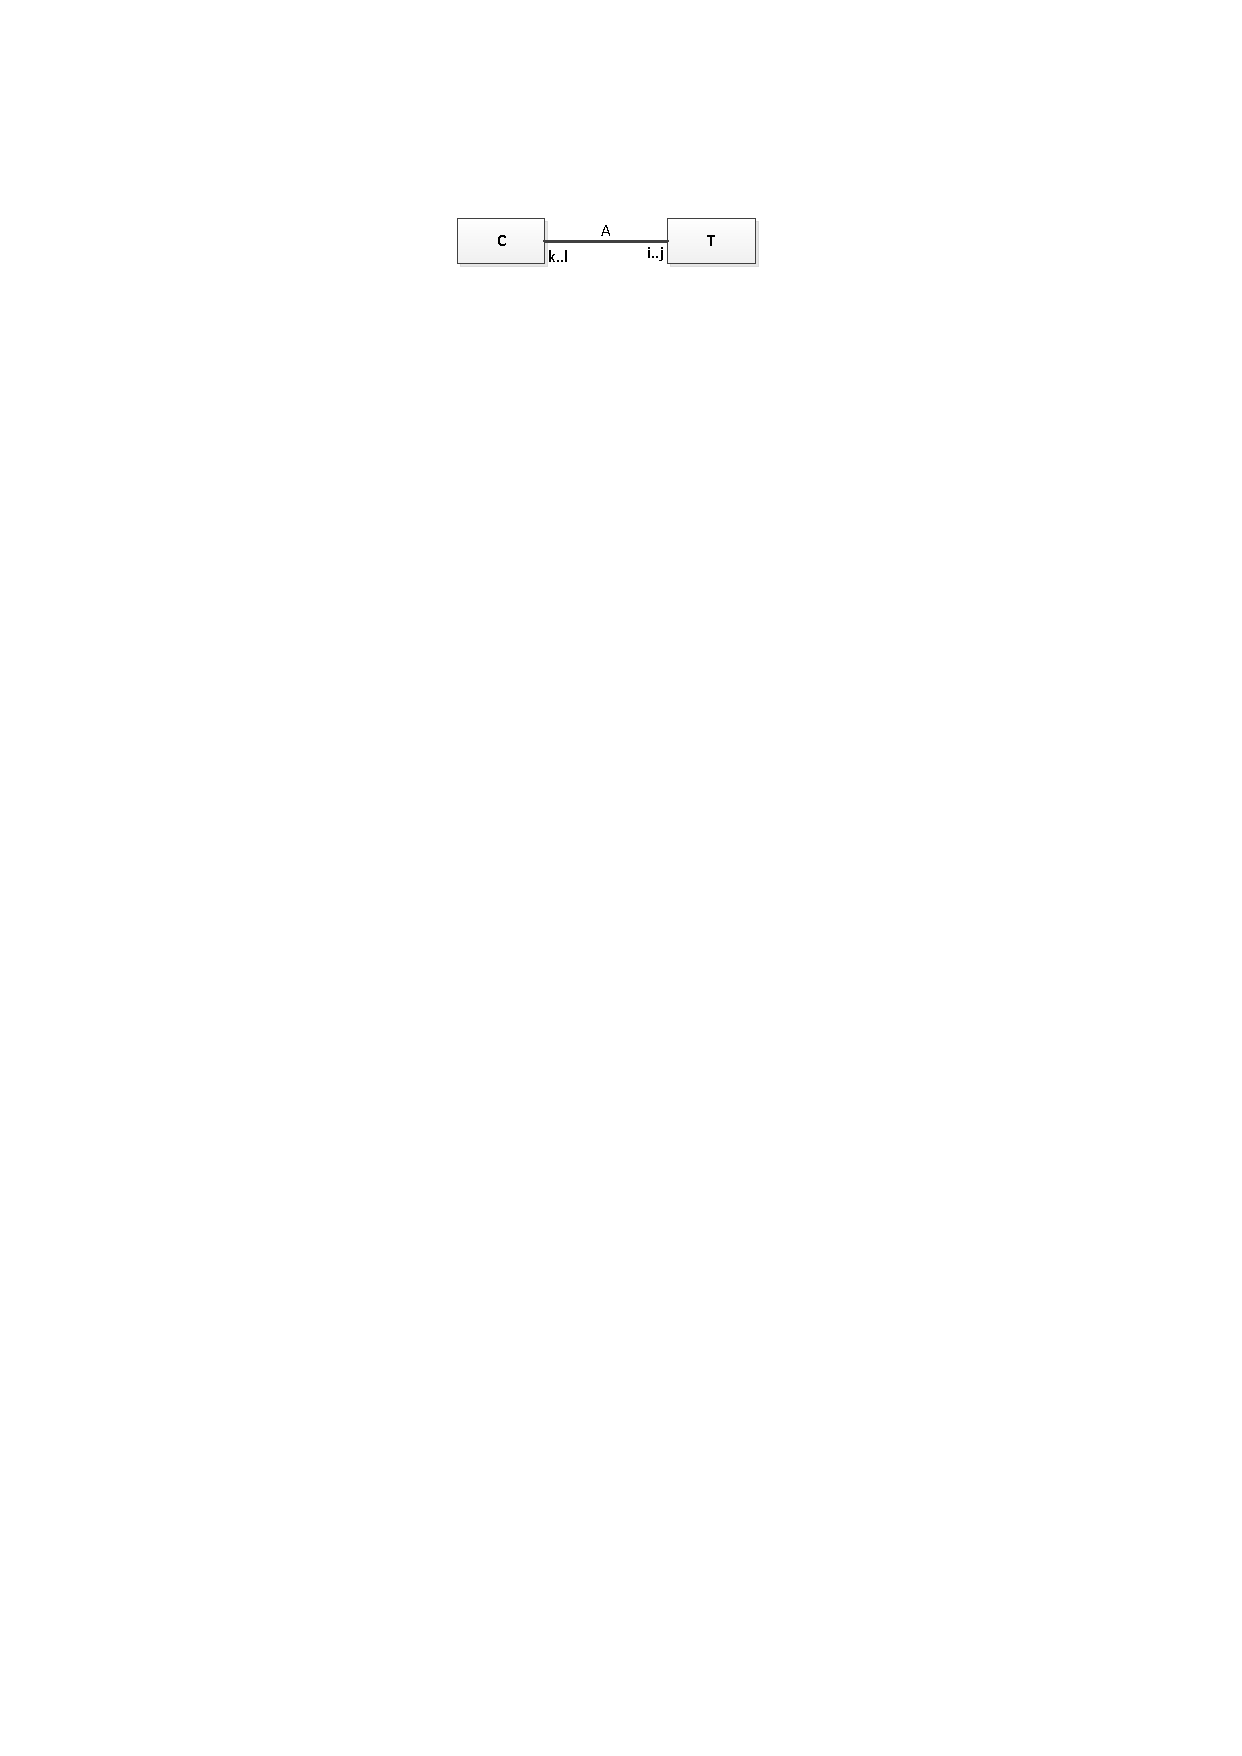
\includegraphics[trim = 77mm 245mm 74mm 25mm, clip, scale=0.75]{./diagrams/chapter5/Association}
      Association \texttt{A} exists between classes \texttt{C} and \texttt{T}
      %Classes \texttt{C1} and \texttt{C2} are disjoint and specialize class \texttt{C} without covering class it 
     \vspace{2mm}
    \end{minipage}
    &
    \begin{minipage}{\dltablespacing}
       $\begin{aligned}   
	  &\exists a.\top \sqsubseteq \hspace*{2pt} C \\
          &\exists a^-.\top \sqsubseteq \hspace*{2pt} T \\
          &C \sqsubseteq (\geq i \hspace*{2pt} a.\top) \sqcap (\leq j \hspace*{2pt} a.\top)\\
          &T \sqsubseteq (\geq k \hspace*{2pt} a^-.\top) \sqcap (\leq l \hspace*{2pt} a^-.\top)\\	  
         \end{aligned}$      
    \end{minipage}
    &
      $\begin{aligned}
        \\
   	&\texttt{ObjectProperty: a}\\[\owlspacing]
    	&\texttt{\hspace*{0.20cm}Domain: C} \\[\owlspacing]
    	&\texttt{\hspace*{0.20cm}Range: T}\\[\owlspacing]
    	&\texttt{ObjectProperty: a\_inv}\\[\owlspacing]
    	&\texttt{\hspace*{0.20cm}InverseOf: a} \\
   	&\texttt{Class: C}\\[\owlspacing]
   	&\texttt{\hspace*{0.20cm}SubClassOf:}\\[\owlspacing]
   	&\texttt{\hspace*{0.40cm}(a min i Thing) and}\\[\owlspacing]
   	&\texttt{\hspace*{0.40cm}(a max j Thing)}\\
   	&\texttt{Class: T}\\[\owlspacing]
   	&\texttt{\hspace*{0.20cm}SubClassOf:}\\[\owlspacing]
   	&\texttt{\hspace*{0.40cm}(a\_inv min k Thing) and}\\[\owlspacing]
   	&\texttt{\hspace*{0.40cm}(a\_inv max l Thing)}\\
   	\\
     \end{aligned}$
    &
    \ref{sec_Binary Associations_Translation} \linebreak p. \pageref{sec_Binary Associations_Translation}, \linebreak \ref{sec_DL Translation in terms of Domain and Range Restrictions}
    \linebreak p. \pageref{sec_DL Translation in terms of Domain and Range Restrictions} \linebreak and \linebreak \ref{subsec_Limiting Redundancy of Assertions}
    \linebreak p. \pageref{subsec_Limiting Redundancy of Assertions}\\       
    \hline  
    \begin{minipage}{\umltablespacing}
      \centering\hspace*{-4mm}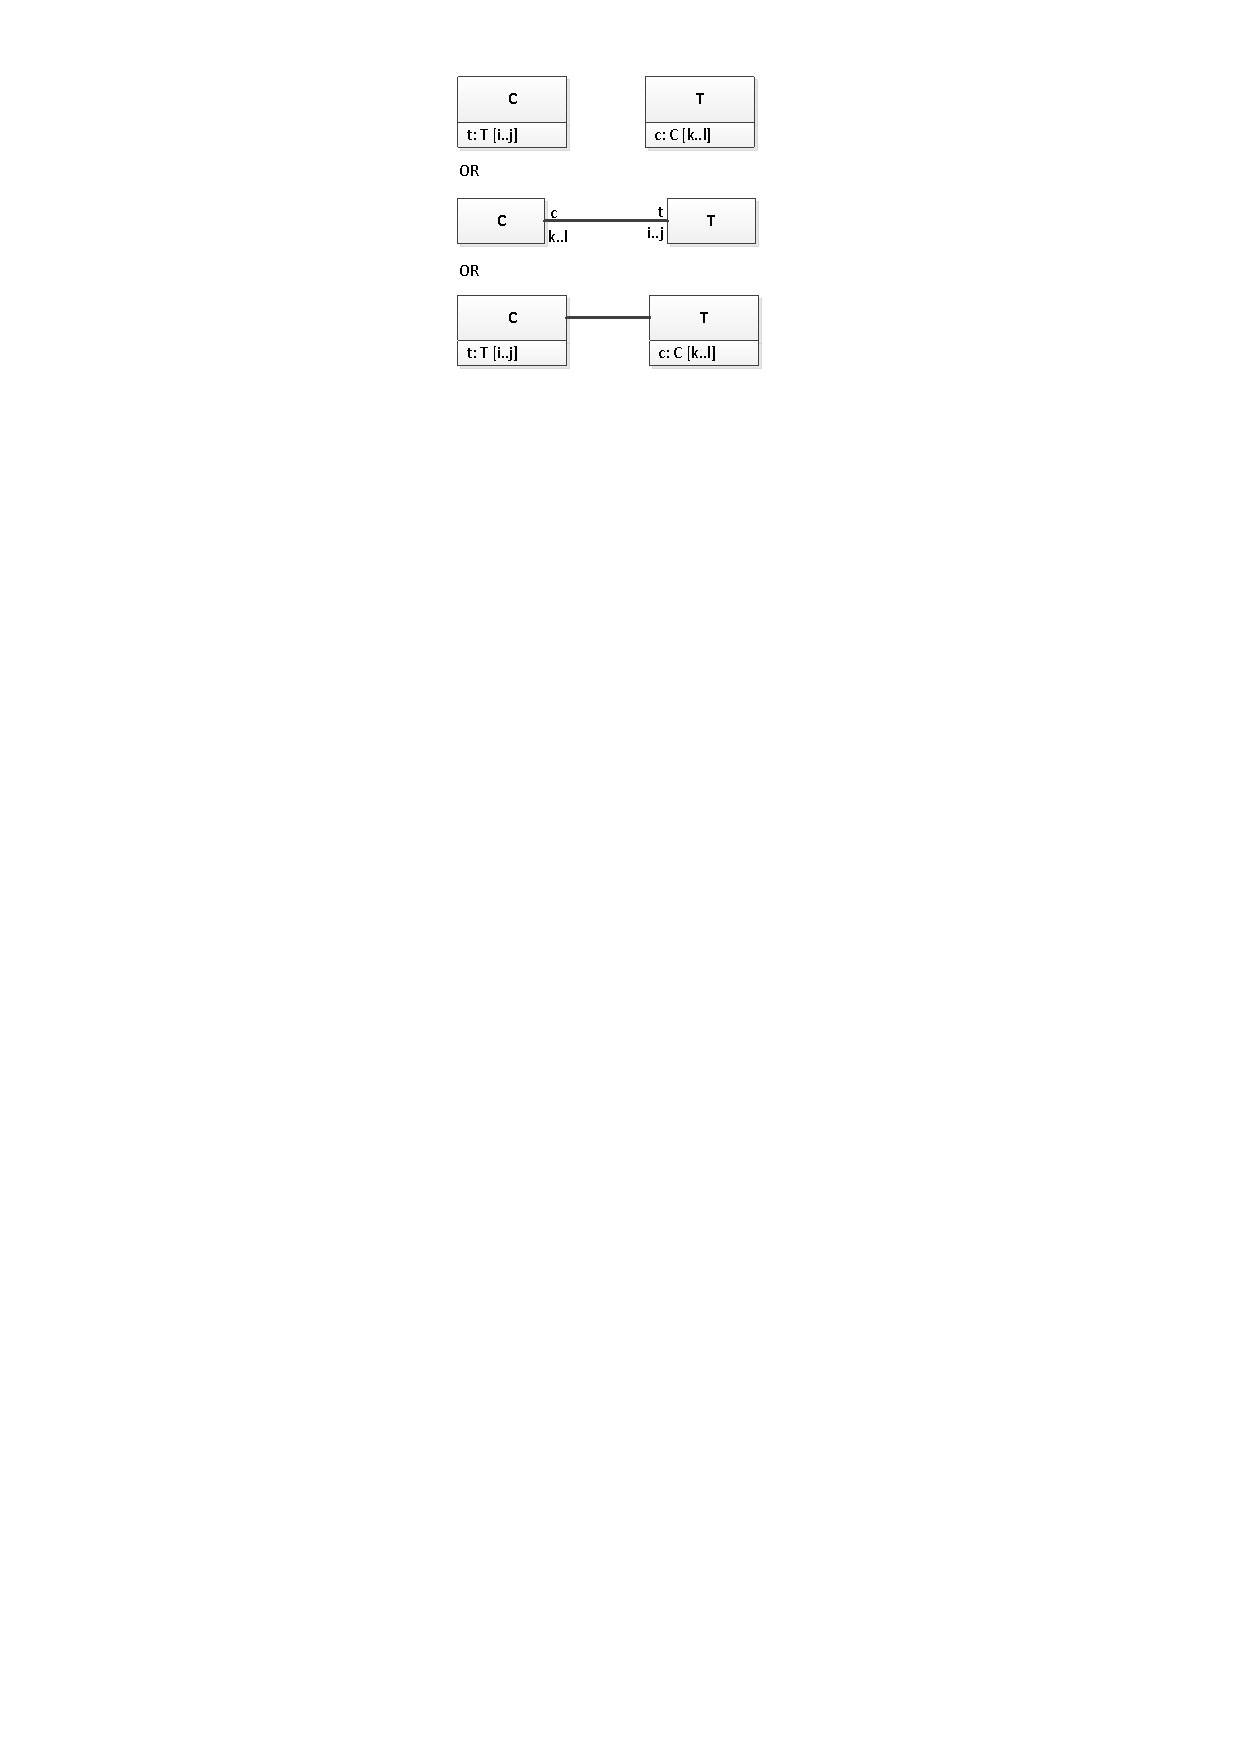
\includegraphics[trim = 77mm 230mm 74mm 5mm, clip, scale=0.75]{./diagrams/chapter5/AssociationEnds}
      Attribute \texttt{t} of type \texttt{T} with multiplicity \texttt{[i..j]} belongs to class \texttt{C}
      and attribute \texttt{c} of type \texttt{C} with multiplicity \texttt{[k..l]} belongs to class \texttt{T}
      \\OR\\
      Association end \texttt{t} with multiplicity \texttt{[i..j]} is associated with class \texttt{C} and asociation end \texttt{c} with multiplicity \texttt{[k..l]} is associated with class \texttt{T}
      \\OR\\
      Line notation is used to make explicit that attributes \texttt{t} and \texttt{c} are also association ends
      %Classes \texttt{C1} and \texttt{C2} are disjoint and specialize class \texttt{C} without covering class it 
     \vspace{2mm}
    \end{minipage}
    &
    \begin{minipage}{\dltablespacing}
       $\begin{aligned}    
	  &\exists t.\top \sqsubseteq \hspace*{2pt} C \\
          &\exists t^-.\top \sqsubseteq \hspace*{2pt} T \\
	  &C \sqsubseteq \hspace*{2pt} (\geq i \hspace*{2pt} t.\top) \hspace*{2pt} \sqcap \hspace*{2pt} (\leq j \hspace*{2pt} t.\top)\\
	  \\
	  &c \equiv t^-\\
	  &T \sqsubseteq \hspace*{2pt} (\geq k \hspace*{2pt} c.\top) \hspace*{2pt} \sqcap \hspace*{2pt} (\leq l \hspace*{2pt} c.\top)\\	  
         \end{aligned}$      
    \end{minipage}
    &
      $\begin{aligned}
         &\texttt{}\\
         &\texttt{ObjectProperty: t} \\[\owlspacing]
         &\texttt{\hspace*{2mm}Domain: C} \\[\owlspacing]
         &\texttt{\hspace*{2mm}Range: T} \\[\owlspacing]
	 &\texttt{Class: C}\\[\owlspacing]
	 &\texttt{\hspace*{2mm}SubClassOf:} \\[\owlspacing]
	 &\texttt{\hspace*{2mm}(t min i Thing) and}\\[\owlspacing]
	 &\texttt{\hspace*{4mm}(t max j Thing)} \\
         &\texttt{ObjectProperty: c} \\[\owlspacing]
         &\texttt{\hspace*{2mm}InverseOf: t}\\[\owlspacing]
	 &\texttt{Class: T}\\[\owlspacing]
	 &\texttt{\hspace*{2mm}SubClassOf:} \\[\owlspacing]
	 &\texttt{\hspace*{2mm}(c min k Thing) and}\\[\owlspacing]
	 &\texttt{\hspace*{4mm}(c max l Thing)} \\[\owlspacing]
   	\\
     \end{aligned}$
    &
    \ref{sec_Binary Associations_Translation} \linebreak p. \pageref{sec_Binary Associations_Translation}, \linebreak \ref{sec_DL Translation in terms of Domain and Range Restrictions}
    \linebreak p. \pageref{sec_DL Translation in terms of Domain and Range Restrictions} \linebreak and \linebreak \ref{sec_On the Equivalence of Attributes and Binary Associations}
    \linebreak p. \pageref{sec_On the Equivalence of Attributes and Binary Associations}\\     
    \hline
    \begin{minipage}{\umltablespacing}
      \centering\hspace*{-4mm}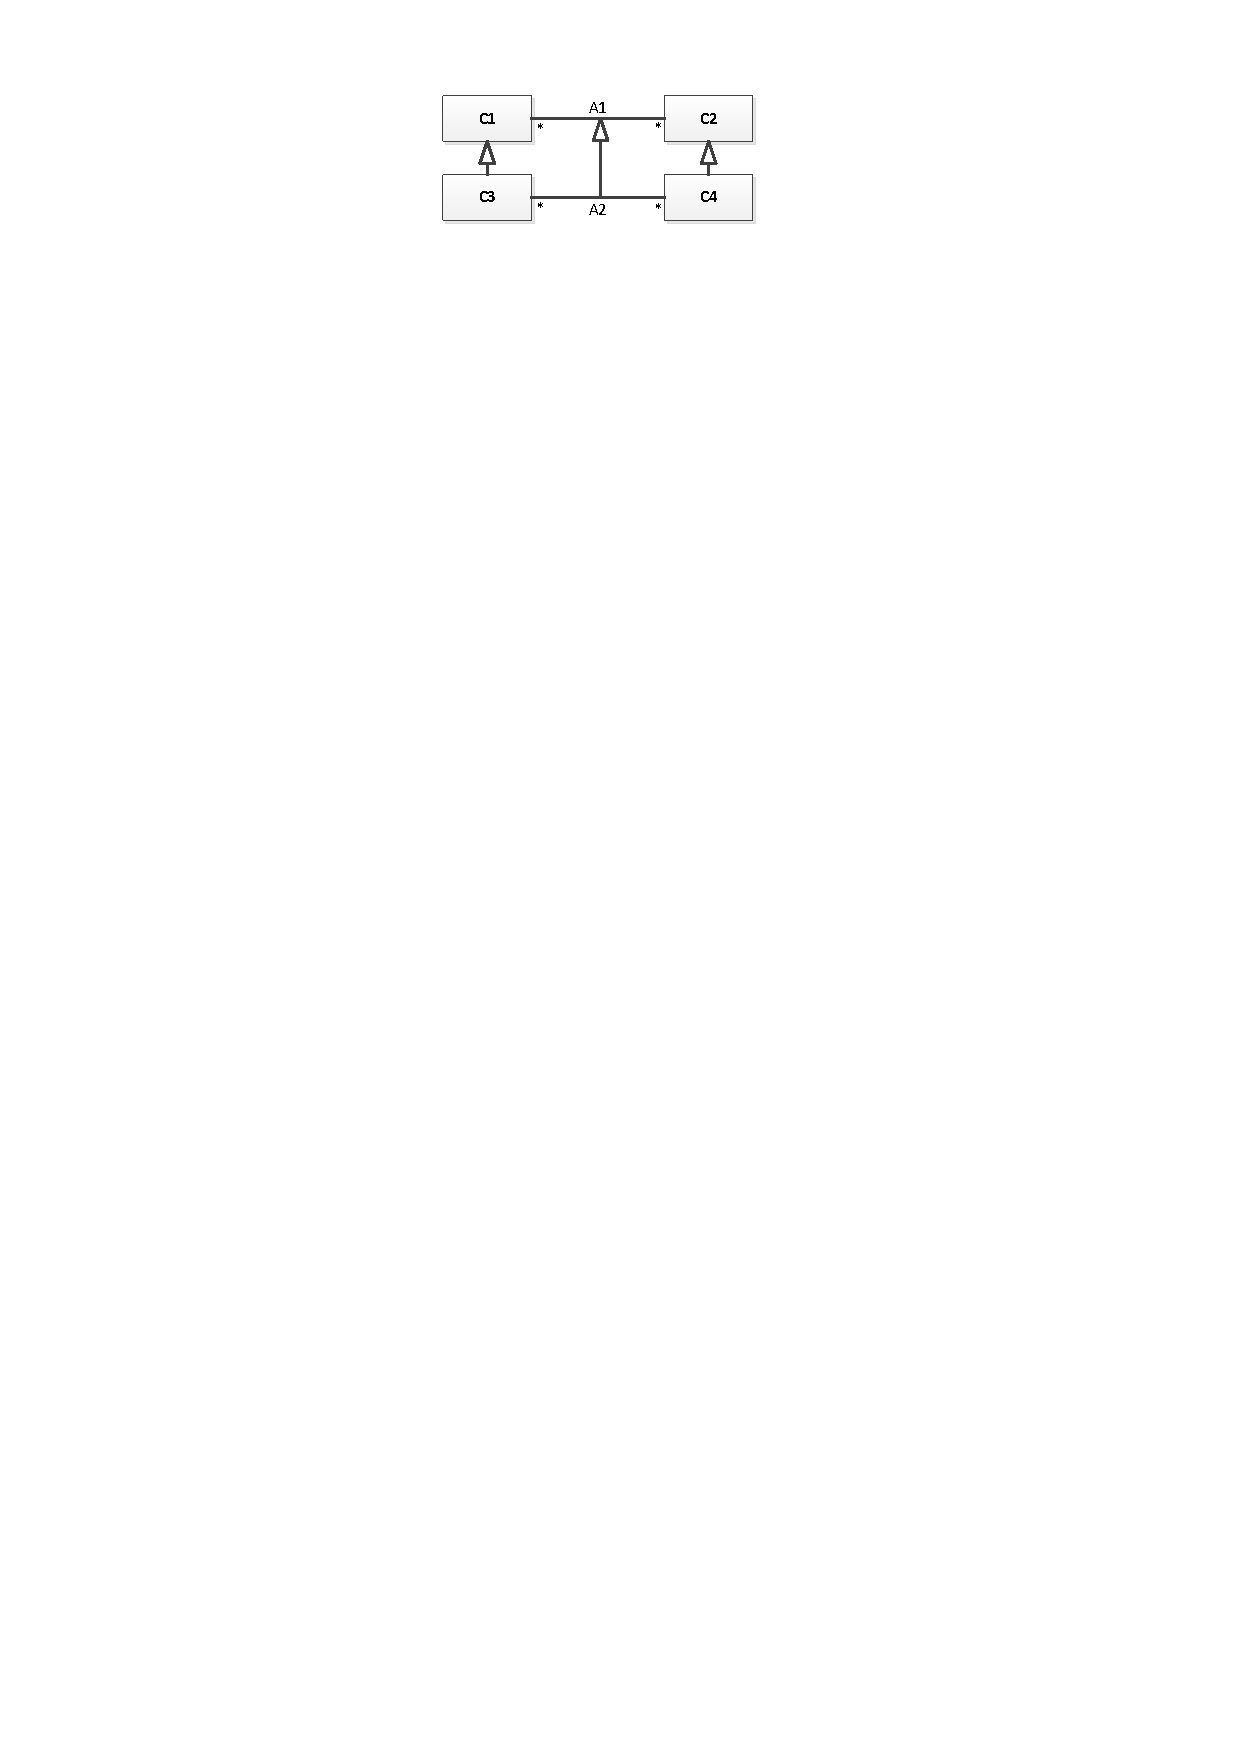
\includegraphics[trim = 75mm 255mm 72mm 5mm, clip, scale=0.75]{./diagrams/chapter5/AssociationSpecialization}
      Association \texttt{A2} specializes association \texttt{A1} 
     \vspace{2mm}
    \end{minipage}
    &
    \begin{minipage}{\dltablespacing}
       $\begin{aligned}    	  
          &\exists a_1.\top \sqsubseteq C_1\\ 
          &\exists a_1^-.\top \sqsubseteq C_2\\
          &\exists a_2.\top \sqsubseteq C_3\\ 
          &\exists a_2^-.\top \sqsubseteq C_4\\
          &a_2 \sqsubseteq a_1\\
         \end{aligned}$      
    \end{minipage}
    &
      $\begin{aligned}
        \\
        &\texttt{Class: C1}\\[\owlspacing]
        &\texttt{Class: C2}\\[\owlspacing]
        &\texttt{Class: C3}\\[\owlspacing]
        &\texttt{Class: C4}\\[\owlspacing]        
        &\texttt{ObjectProperty: a1}\\[\owlspacing]
        &\texttt{\hspace*{2mm}Domain: C1} \\[\owlspacing]
        &\texttt{\hspace*{2mm}Range: C2} \\[\owlspacing]
   	&\texttt{ObjectProperty: a2}\\[\owlspacing]
        &\texttt{\hspace*{2mm}Domain: C3} \\[\owlspacing]
        &\texttt{\hspace*{2mm}Range: C4} \\[\owlspacing]   	
    	&\texttt{\hspace*{2mm}SubPropertyOf: a1} \\
    	&\texttt{}\\
     \end{aligned}$
    &
    \ref{sec_Association_Specialization} \linebreak p. \pageref{sec_Association_Specialization} \linebreak and \linebreak \ref{subsec_Limiting Redundancy of Assertions} \linebreak 
    p. \pageref{subsec_Limiting Redundancy of Assertions}\\ 
    
    \hline
    \begin{minipage}{\umltablespacing}
      \centering\hspace*{-6.3mm}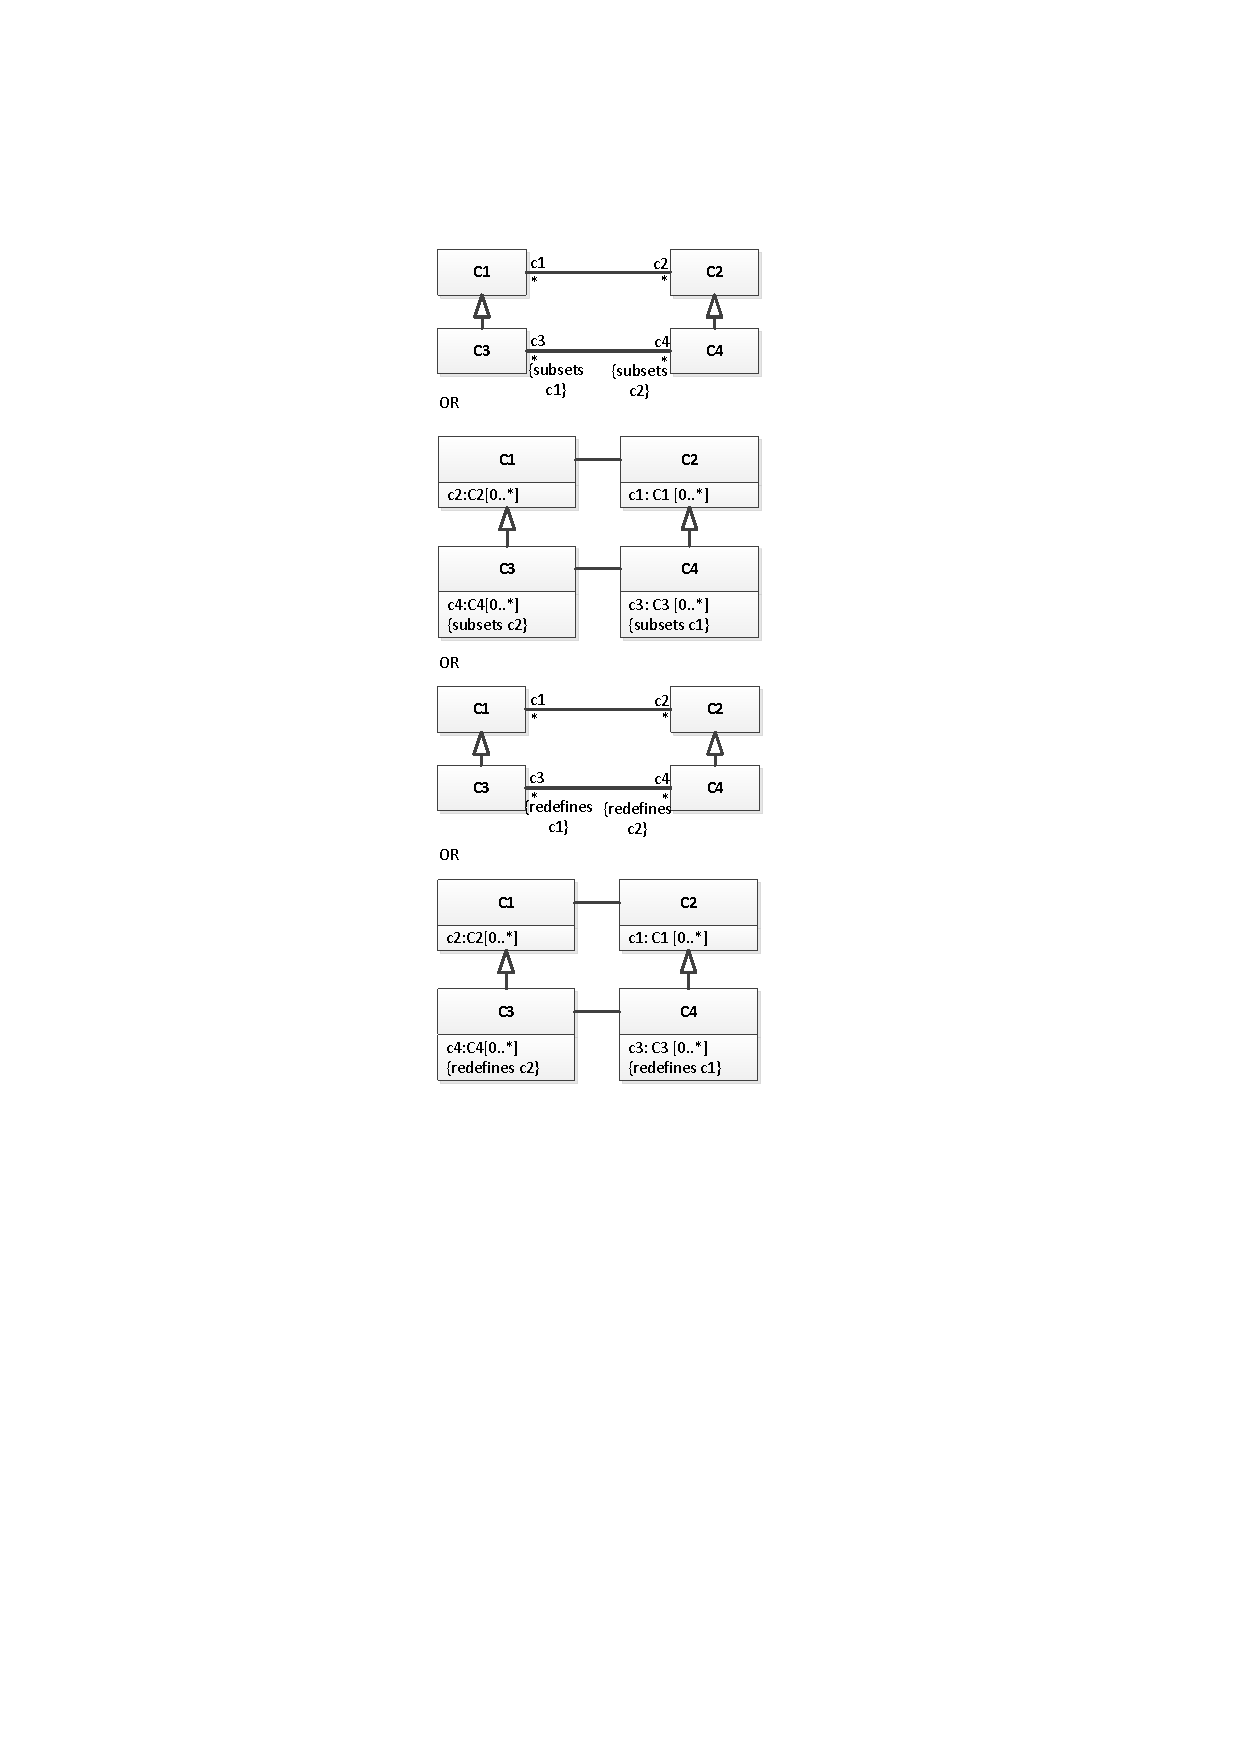
\includegraphics[trim = 72mm 110mm 81mm 35mm, clip, scale=0.75]{./diagrams/chapter5/AssociationAttributeSpecialization}
      Association end (resp. attribute) \texttt{c3} subsets association end (resp. attribute) \texttt{c1} and association end (resp. attribute) \texttt{c4} subsets association end (resp. attribute) \texttt{c2}
      \\OR\\
      Association end (resp. attribute) \texttt{c3} redefines association end (resp. attribute) \texttt{c1} and association end (resp. attribute) \texttt{c4} redefines association end (resp. attribute) \texttt{c2}      
     \vspace{2mm}
    \end{minipage}
    &
    \begin{minipage}{\dltablespacing}
       $\begin{aligned}    	  
    	c_1 &\equiv c_2^-\\ 
    	\exists c_1.\top &\sqsubseteq C_1\\
    	\exists c_1^-.\top &\sqsubseteq C_2\\
    	c_3 &\equiv c_4^-\\
    	\exists c_3.\top &\sqsubseteq C_3\\
    	\exists c_3^-.\top &\sqsubseteq C_4\\    	
    	c_3 &\sqsubseteq c_1\\
    	c_4 &\sqsubseteq c_2  
         \end{aligned}$      
    \end{minipage}
    &
      $\begin{aligned}
        \\
        &\texttt{Class: C1}\\[\owlspacing]
        &\texttt{Class: C2}\\[\owlspacing]
        &\texttt{Class: C3}\\[\owlspacing]
        &\texttt{Class: C4}\\[\owlspacing]
   	&\texttt{ObjectProperty: c1}\\[\owlspacing]
   	&\texttt{\hspace*{0.20cm} Domain: C1}\\[\owlspacing]
   	&\texttt{\hspace*{0.20cm} Range: C2}\\[\owlspacing]
   	&\texttt{\hspace*{0.20cm} InverseOf: c2}\\[\owlspacing]
   	&\texttt{ObjectProperty: c2}\\[\owlspacing]
   	&\texttt{ObjectProperty: c3}\\[\owlspacing]
   	&\texttt{\hspace*{0.20cm} Domain: C3}\\[\owlspacing]
   	&\texttt{\hspace*{0.20cm} Range: C4}\\[\owlspacing]
   	&\texttt{\hspace*{0.20cm} InverseOf: c4}\\[\owlspacing] 
    	&\texttt{\hspace*{0.20cm} SubPropertyOf: c1}\\[\owlspacing]
    	&\texttt{ObjectProperty: c4}\\[\owlspacing]
   	\\
     \end{aligned}$
    &
    \ref{sec_Subsetting and Redefinition of Association Ends}
    \linebreak p. \pageref{sec_Subsetting and Redefinition of Association Ends}\\        
    \hline
    \begin{minipage}{\umltablespacing}
      \centering\hspace*{-4mm}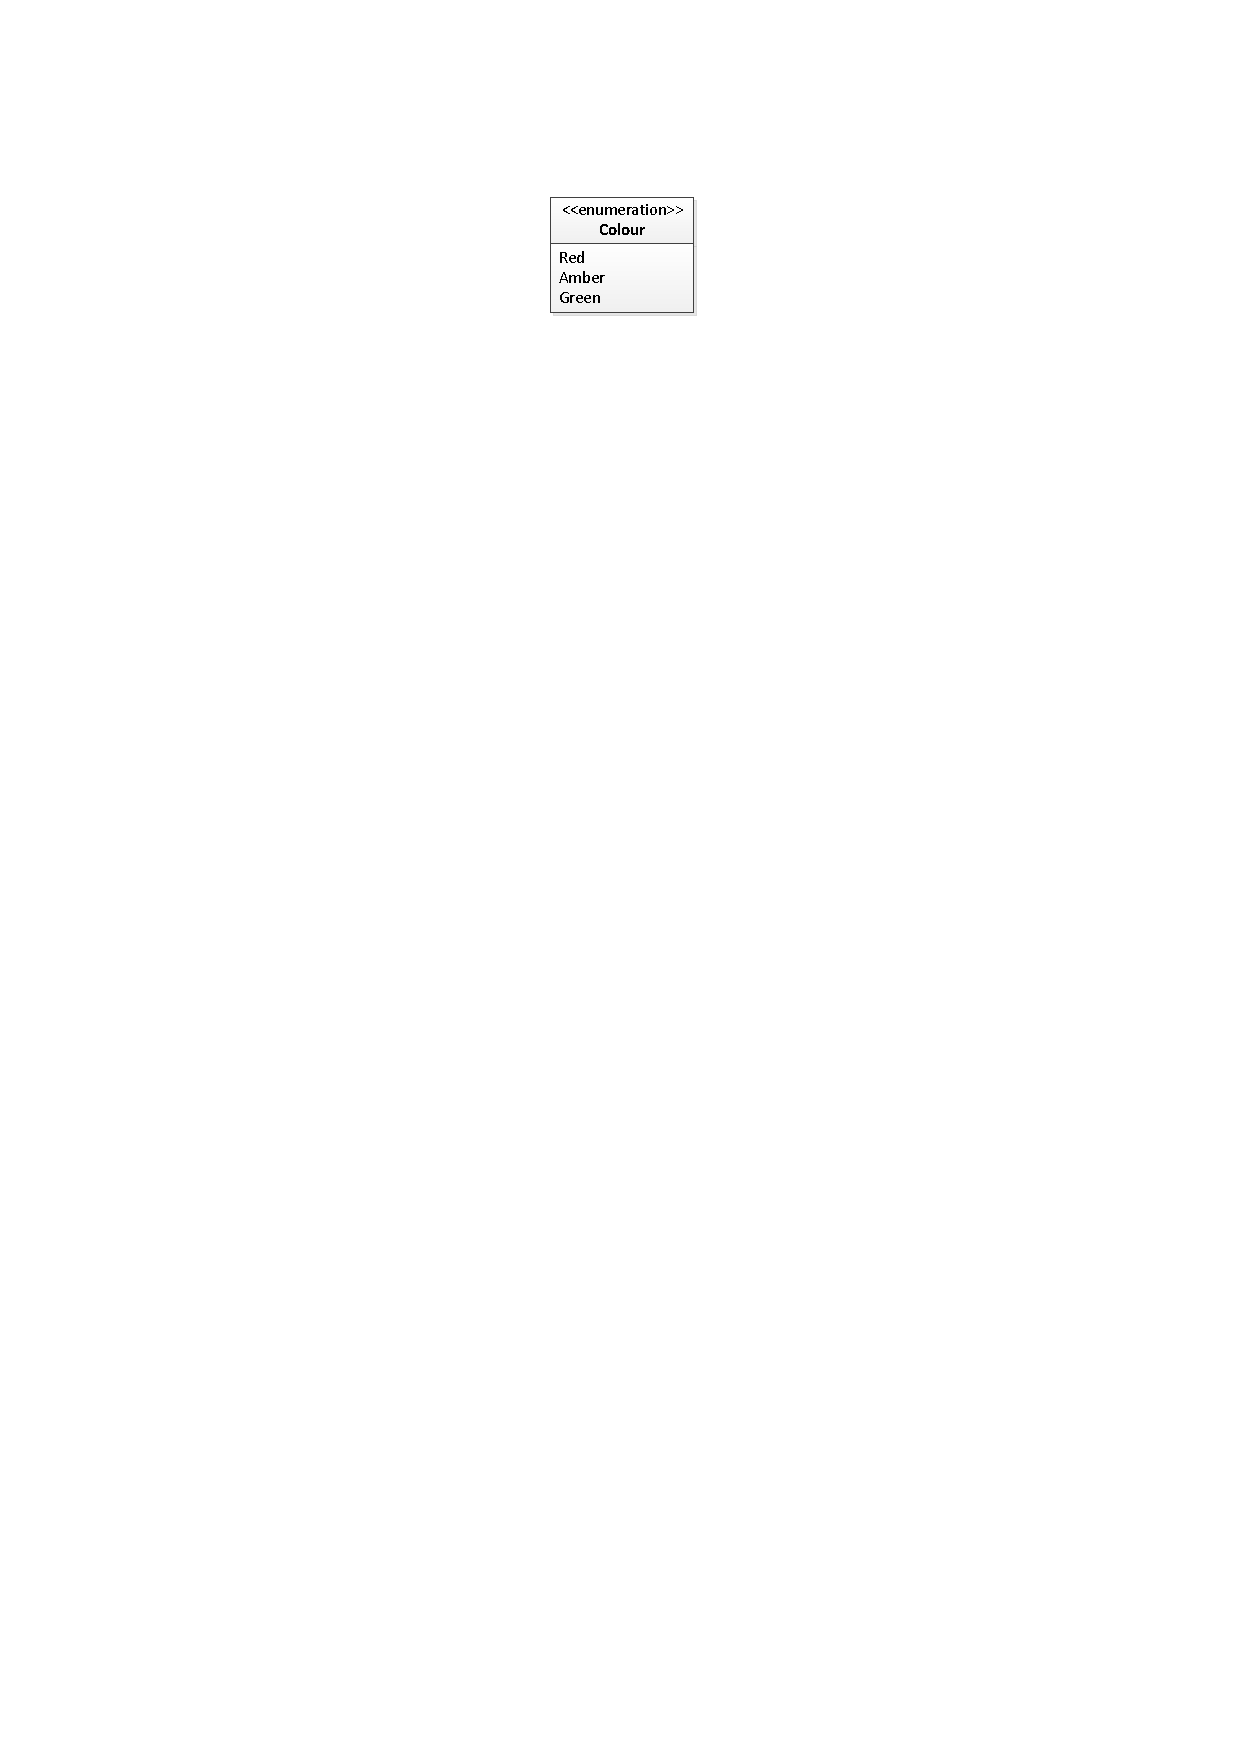
\includegraphics[trim = 80mm 239mm 72mm 25mm, clip, scale=0.75]{./diagrams/chapter5/Enumeration}
      The \texttt{Colour} enumeration consists of the colours \texttt{Red}, \texttt{Amber} and \texttt{Green}
     \vspace{2mm}
    \end{minipage}
    &
    $\begin{aligned}
    Colour &\equiv \{Green, Amber, Red\}\\
    Green &\not\approx Amber\\
    Green &\not\approx Red \\
    Amber &\not\approx Red
    \end{aligned}$
    &
      $\begin{aligned}
      \\
         &\texttt{Class: Colour}\\[\owlspacing]
         &\texttt{\hspace*{2mm} EquivalentTo:}\\[\owlspacing]
         &\texttt{\hspace*{4mm}\{Green, Amber, Red\}}\\[\owlspacing]
         &\texttt{Individual: Green}\\[\owlspacing]
         &\texttt{\hspace*{2mm} Types: Colour}\\[\owlspacing]
         &\texttt{Individual: Amber}\\[\owlspacing]
         &\texttt{\hspace*{2mm} Types: Colour}\\[\owlspacing]
         &\texttt{Individual: Red}\\[\owlspacing]
         &\texttt{\hspace*{2mm} Types: Colour}\\[\owlspacing]
         &\texttt{DifferentIndividuals: }\\[\owlspacing]
         &\texttt{\hspace*{2mm} Green, Amber, Red}\\
     \end{aligned}$
    &
    \ref{sec_Enumerations} \linebreak p. \pageref{sec_Enumerations}\\     
    \hline            
    \begin{minipage}{\umltablespacing}
      \centering\hspace*{-5.5mm}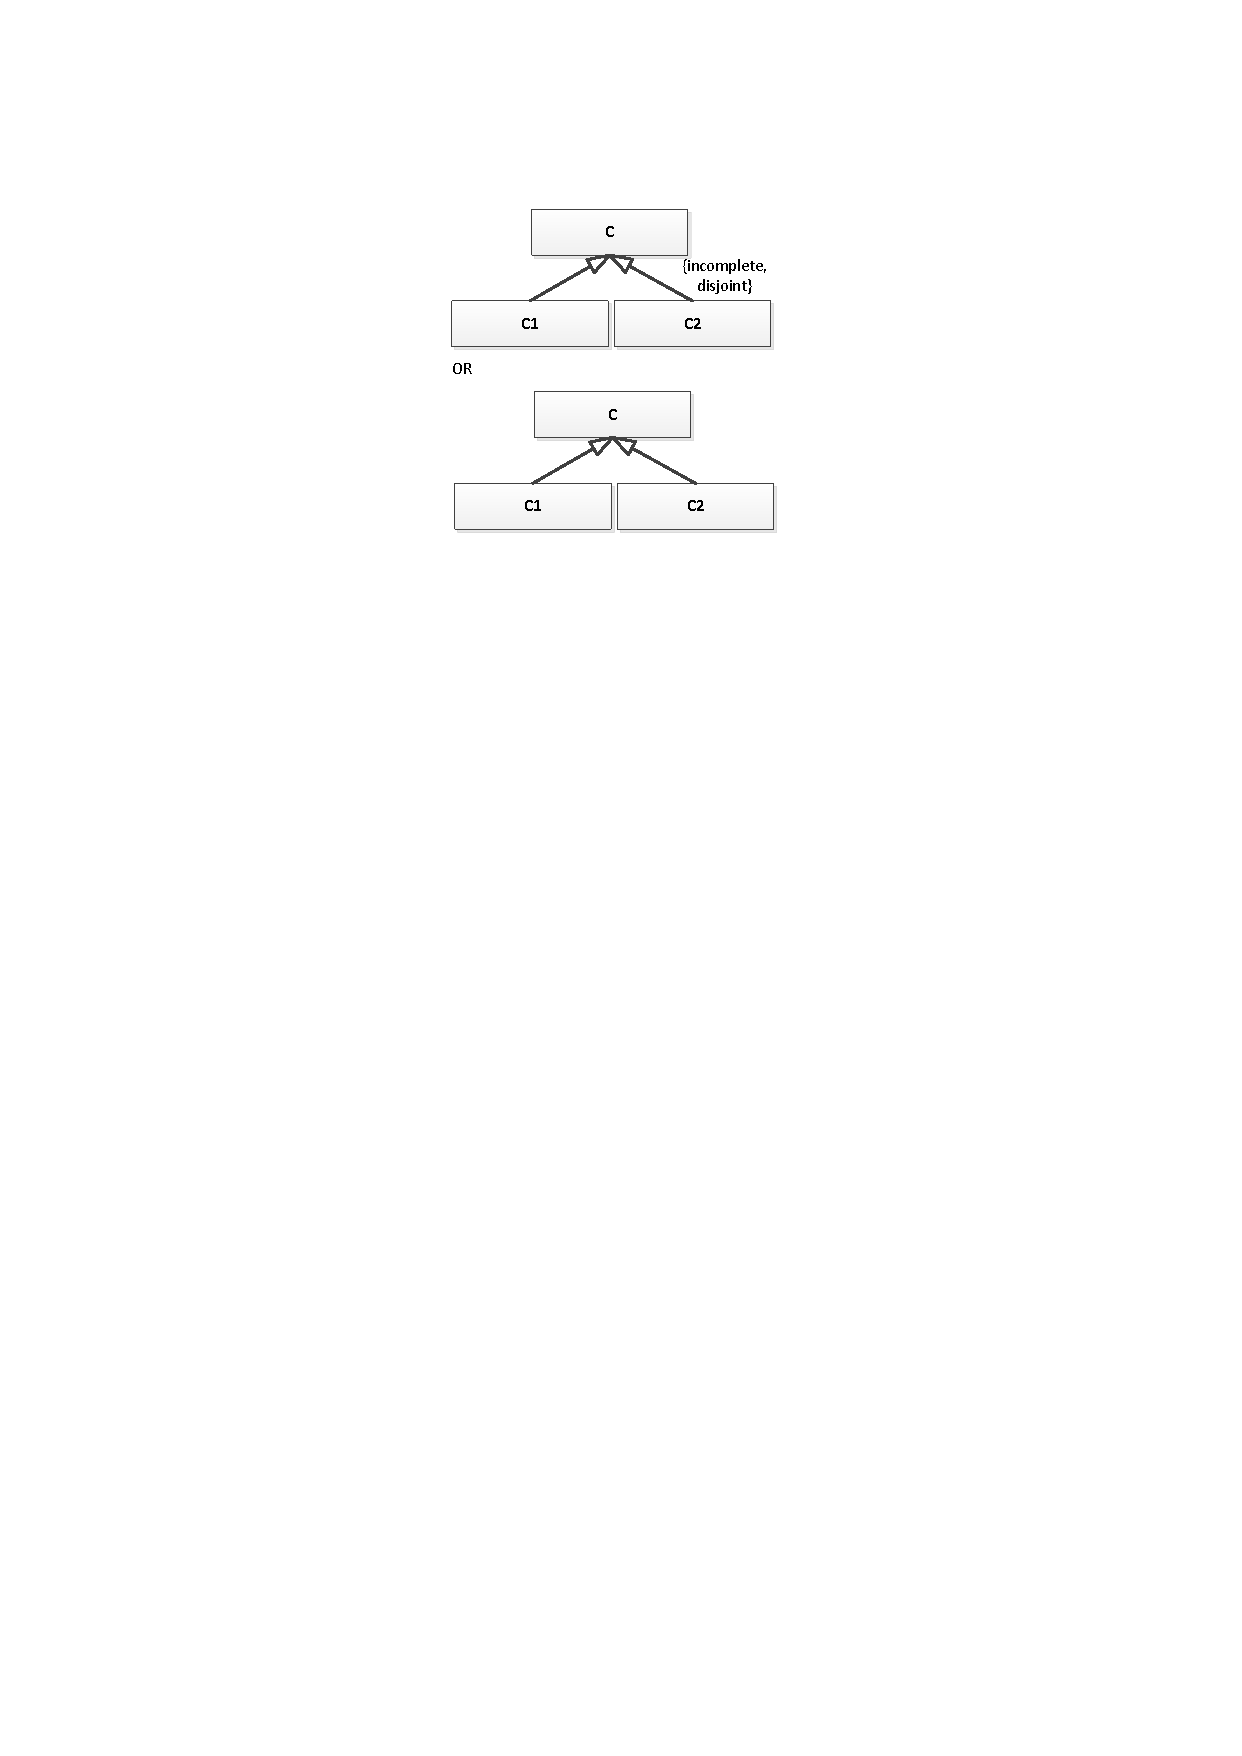
\includegraphics[trim = 76mm 205mm 72mm 25mm, clip, scale=0.75]{./diagrams/chapter5/IncompleteDisjoint}
      Class \texttt{C} is specialized by the disjoint classes \texttt{C1} and \texttt{C2} which do not cover class \texttt{C}
      %Classes \texttt{C1} and \texttt{C2} are disjoint and specialize class \texttt{C} without covering class it 
     \vspace{2mm}
    \end{minipage}
    &
    \begin{minipage}{\dltablespacing}
       $\begin{aligned}    
	  &C_1 \sqsubseteq C  \\  
	  &C_2 \sqsubseteq C \\
	  &C_1 \sqsubseteq \neg C_2
         \end{aligned}$      
    \end{minipage}
    &
      $\begin{aligned}
	  &\texttt{Class: C}\\[\owlspacing]
          &\texttt{Class: C1}\\[\owlspacing]
	  &\texttt{\hspace*{0.20cm}SubClassOf: C}\\[\owlspacing]
          &\texttt{Class: C2}\\[\owlspacing]
          &\texttt{\hspace*{0.20cm}SubClassOf: C}\\[\owlspacing]
          &\texttt{DisjointClasses:}\\[\owlspacing]
          &\texttt{\hspace*{0.20cm}C1, C2}
     \end{aligned}$
    &
    \ref{sec_Generalization/Specialization of Classes} \linebreak p. \pageref{sec_Generalization/Specialization of Classes}\\
     \hline
    \begin{minipage}{\umltablespacing}
      \centering\hspace*{-5.5mm}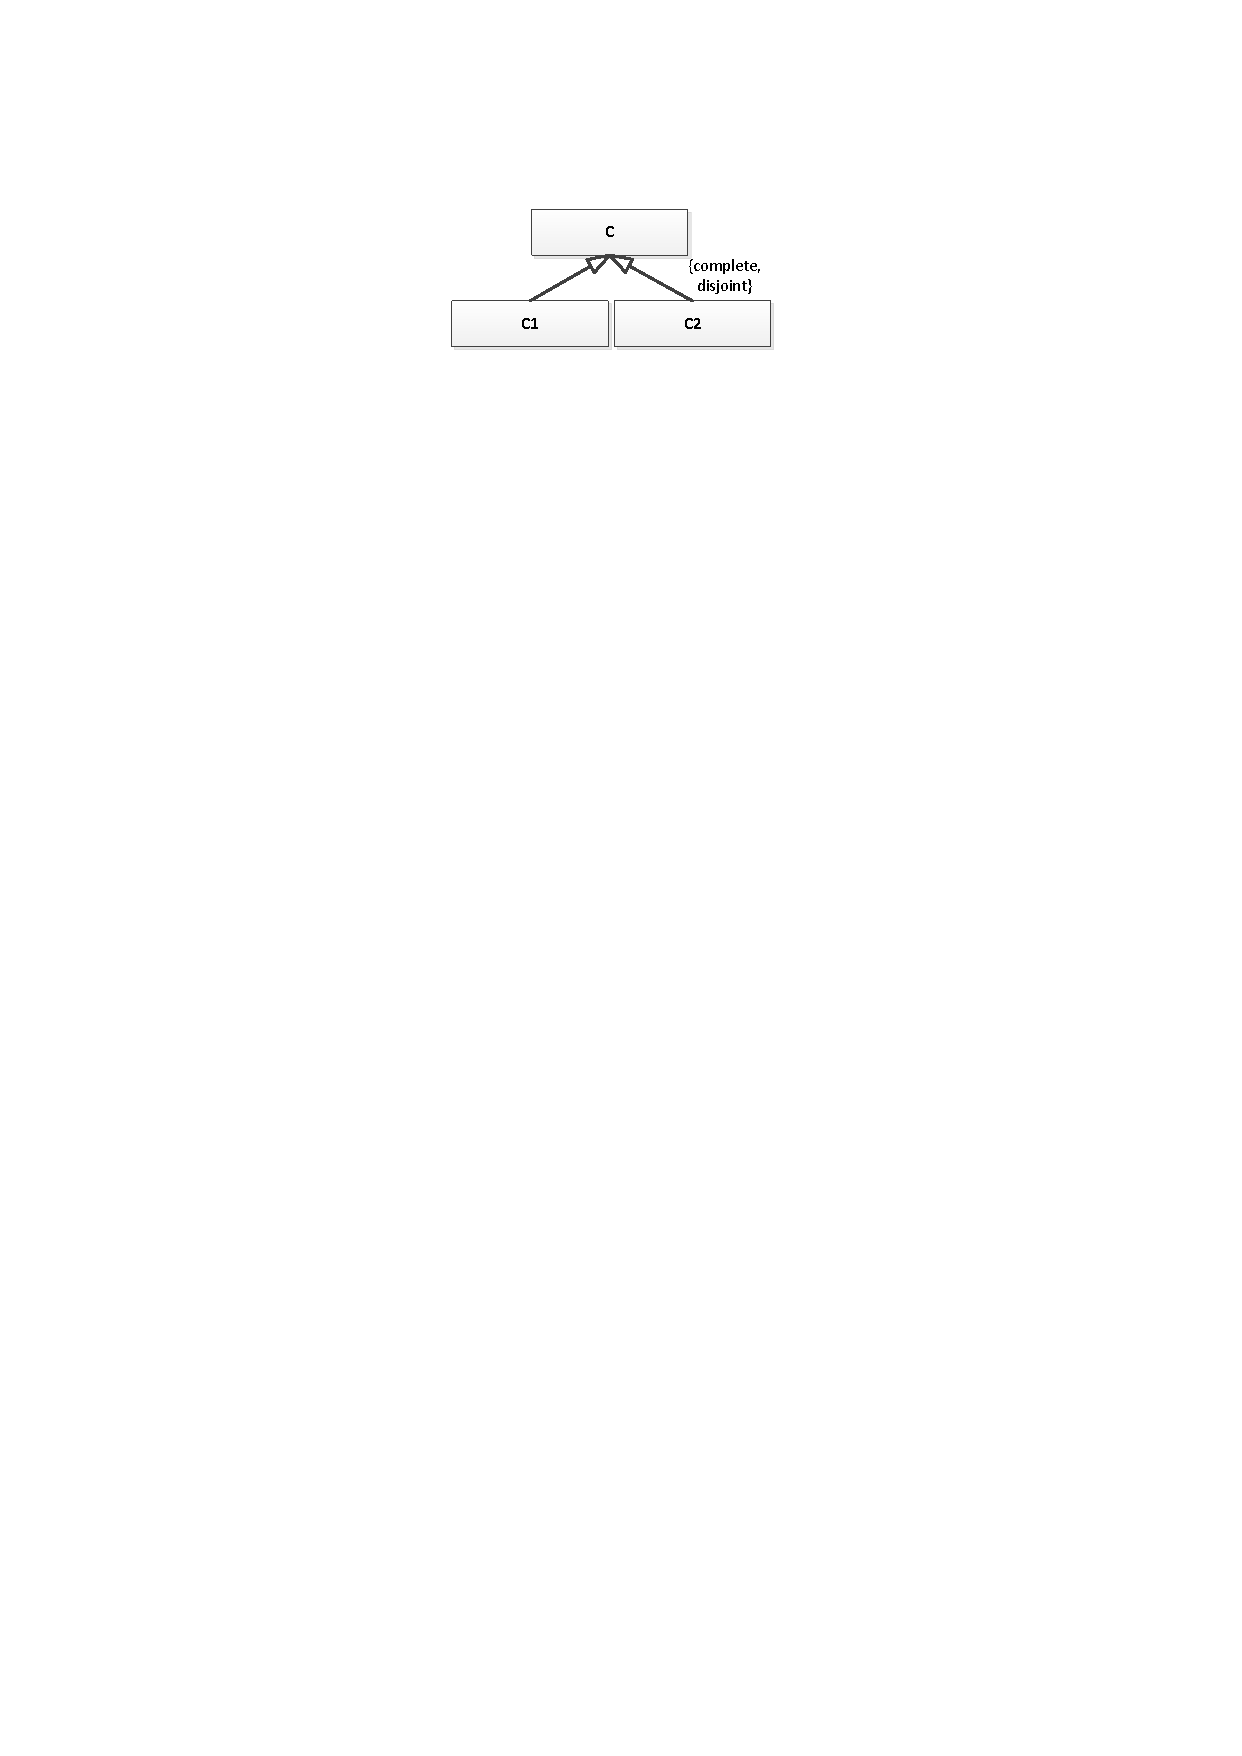
\includegraphics[trim = 76mm 235mm 72mm 25mm, clip, scale=0.75]{./diagrams/chapter5/CompleteDisjoint}
      Class \texttt{C} is specialized by the disjoint classes \texttt{C1} and \texttt{C2} which cover class \texttt{C}  
     \vspace{2mm}
    \end{minipage}
    &
    \begin{minipage}{\dltablespacing}
       $\begin{aligned}   
	  &C \sqsubseteq C_1 \sqcup C_2\\
	  &C_1 \sqsubseteq \neg C_2\\
	  &C_1 \sqsubseteq C  \\  
	  &C_2 \sqsubseteq C 
       \end{aligned}$     
    \end{minipage}
    &
      $\begin{aligned}
	  &\texttt{Class: C}\\[\owlspacing]
	  &\texttt{\hspace*{0.20cm}DisjointUnionOf:}\\[\owlspacing]
	  &\texttt{\hspace*{0.40cm}C1, C2}\\[\owlspacing]
          &\texttt{Class: C1}\\[\owlspacing]
	  &\texttt{\hspace*{0.20cm}SubClassOf: C}\\[\owlspacing]
          &\texttt{Class: C2}\\[\owlspacing]
          &\texttt{\hspace*{0.20cm}SubClassOf: C}	
     \end{aligned}$
    &
    \ref{sec_Generalization/Specialization of Classes} \linebreak p. \pageref{sec_Generalization/Specialization of Classes}\\
     \hline     
    \begin{minipage}{\umltablespacing}
      \centering\hspace*{-5.5mm}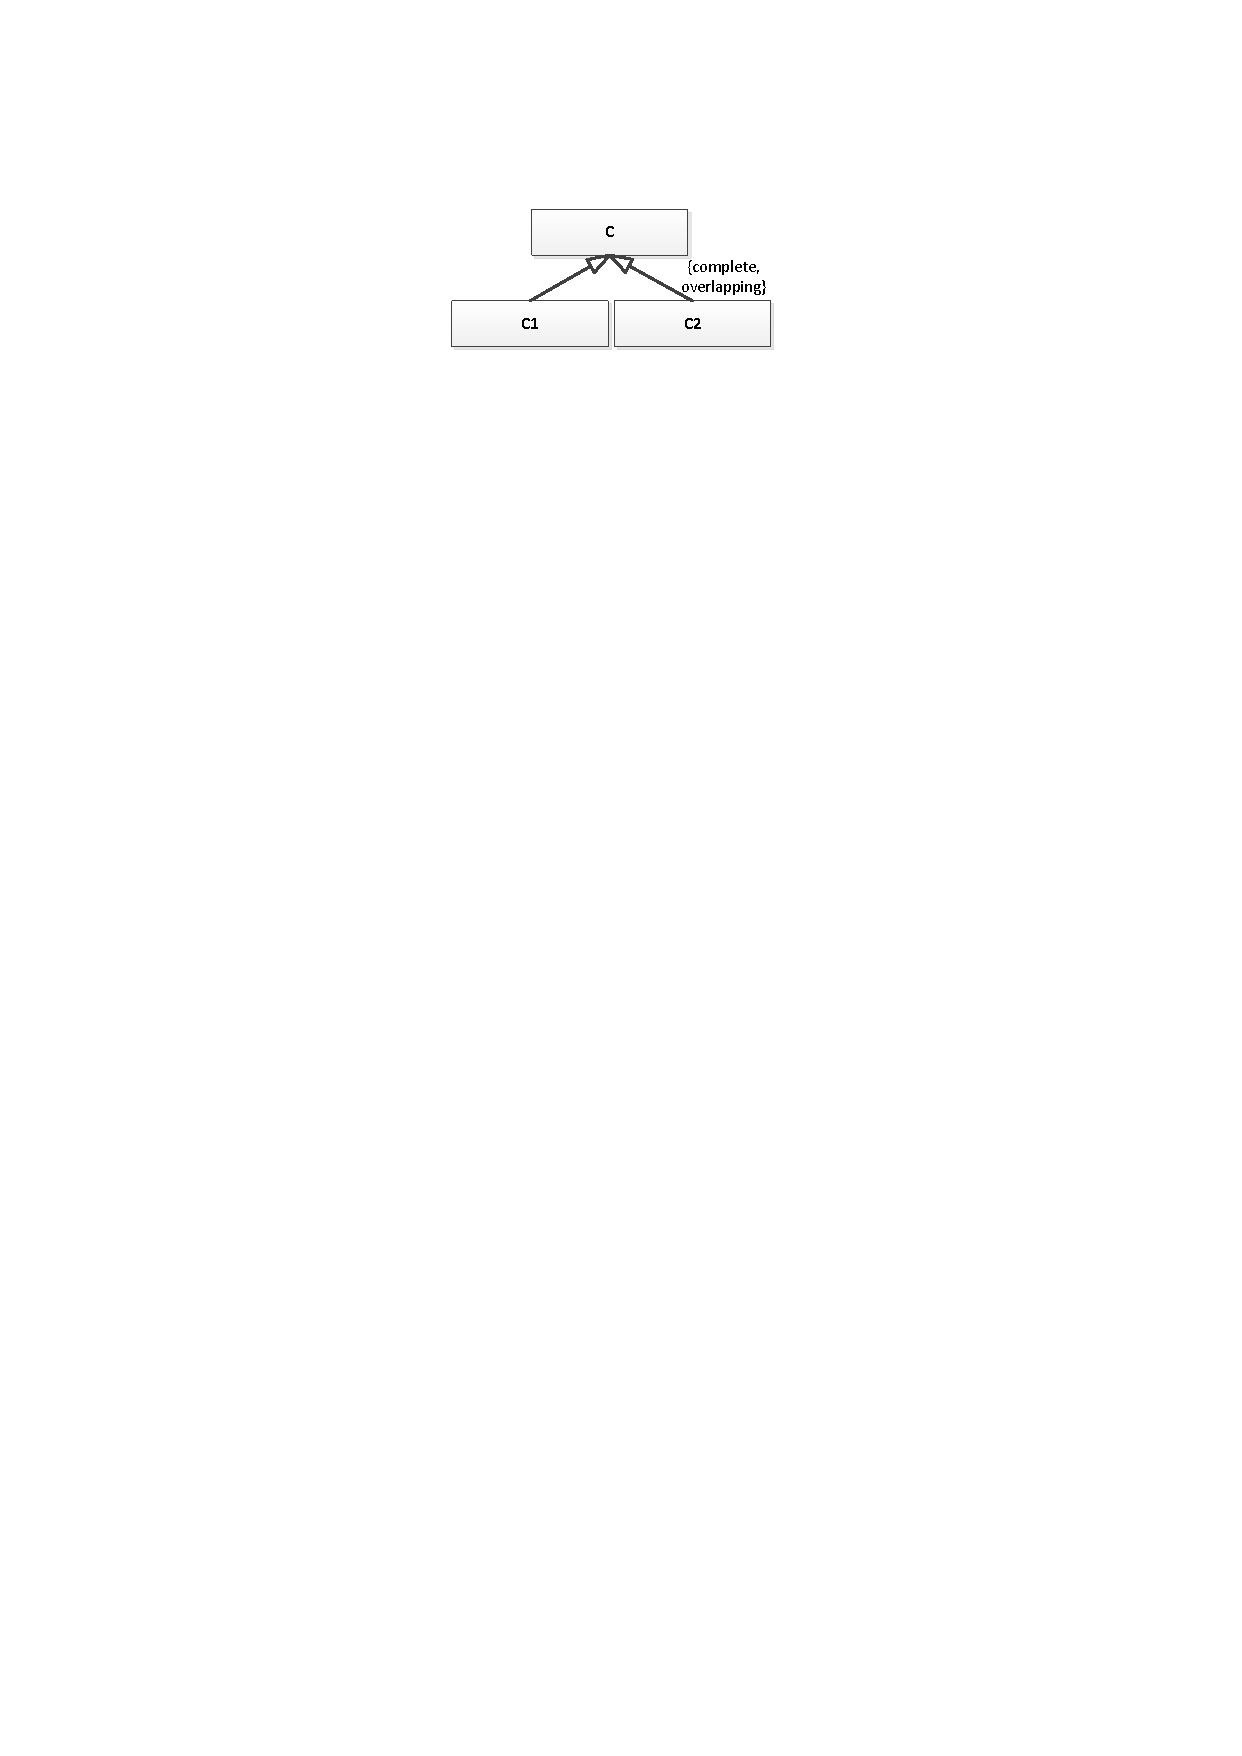
\includegraphics[trim = 76mm 235mm 72mm 25mm, clip, scale=0.75]{./diagrams/chapter5/CompleteOverlapping}
      Class \texttt{C} is specialized by the overlapping classes \texttt{C1} and \texttt{C2} which cover class \texttt{C}  
     \vspace{2mm}
    \end{minipage}
    &
    \begin{minipage}{\dltablespacing}
       $\begin{aligned}   
	  &C \sqsubseteq C_1 \sqcup C_2\\
	  &C_1 \sqsubseteq C  \\  
	  &C_2 \sqsubseteq C 
       \end{aligned}$     
    \end{minipage}
    &
      $\begin{aligned}
	  &\texttt{Class: C}\\[\owlspacing]
	  &\texttt{\hspace*{0.20cm}SubClassOf:}\\[\owlspacing]
	  &\texttt{\hspace*{0.40cm}C1 or C2}\\[\owlspacing]
          &\texttt{Class: C1}\\[\owlspacing]
	  &\texttt{\hspace*{0.20cm}SubClassOf: C}\\[\owlspacing]
          &\texttt{Class: C2}\\[\owlspacing]
          &\texttt{\hspace*{0.20cm}SubClassOf: C}	
     \end{aligned}$
    &
    \ref{sec_Generalization/Specialization of Classes} \linebreak p. \pageref{sec_Generalization/Specialization of Classes}\\
     \hline     
    \begin{minipage}{\umltablespacing}
      \centering\hspace*{-5.5mm}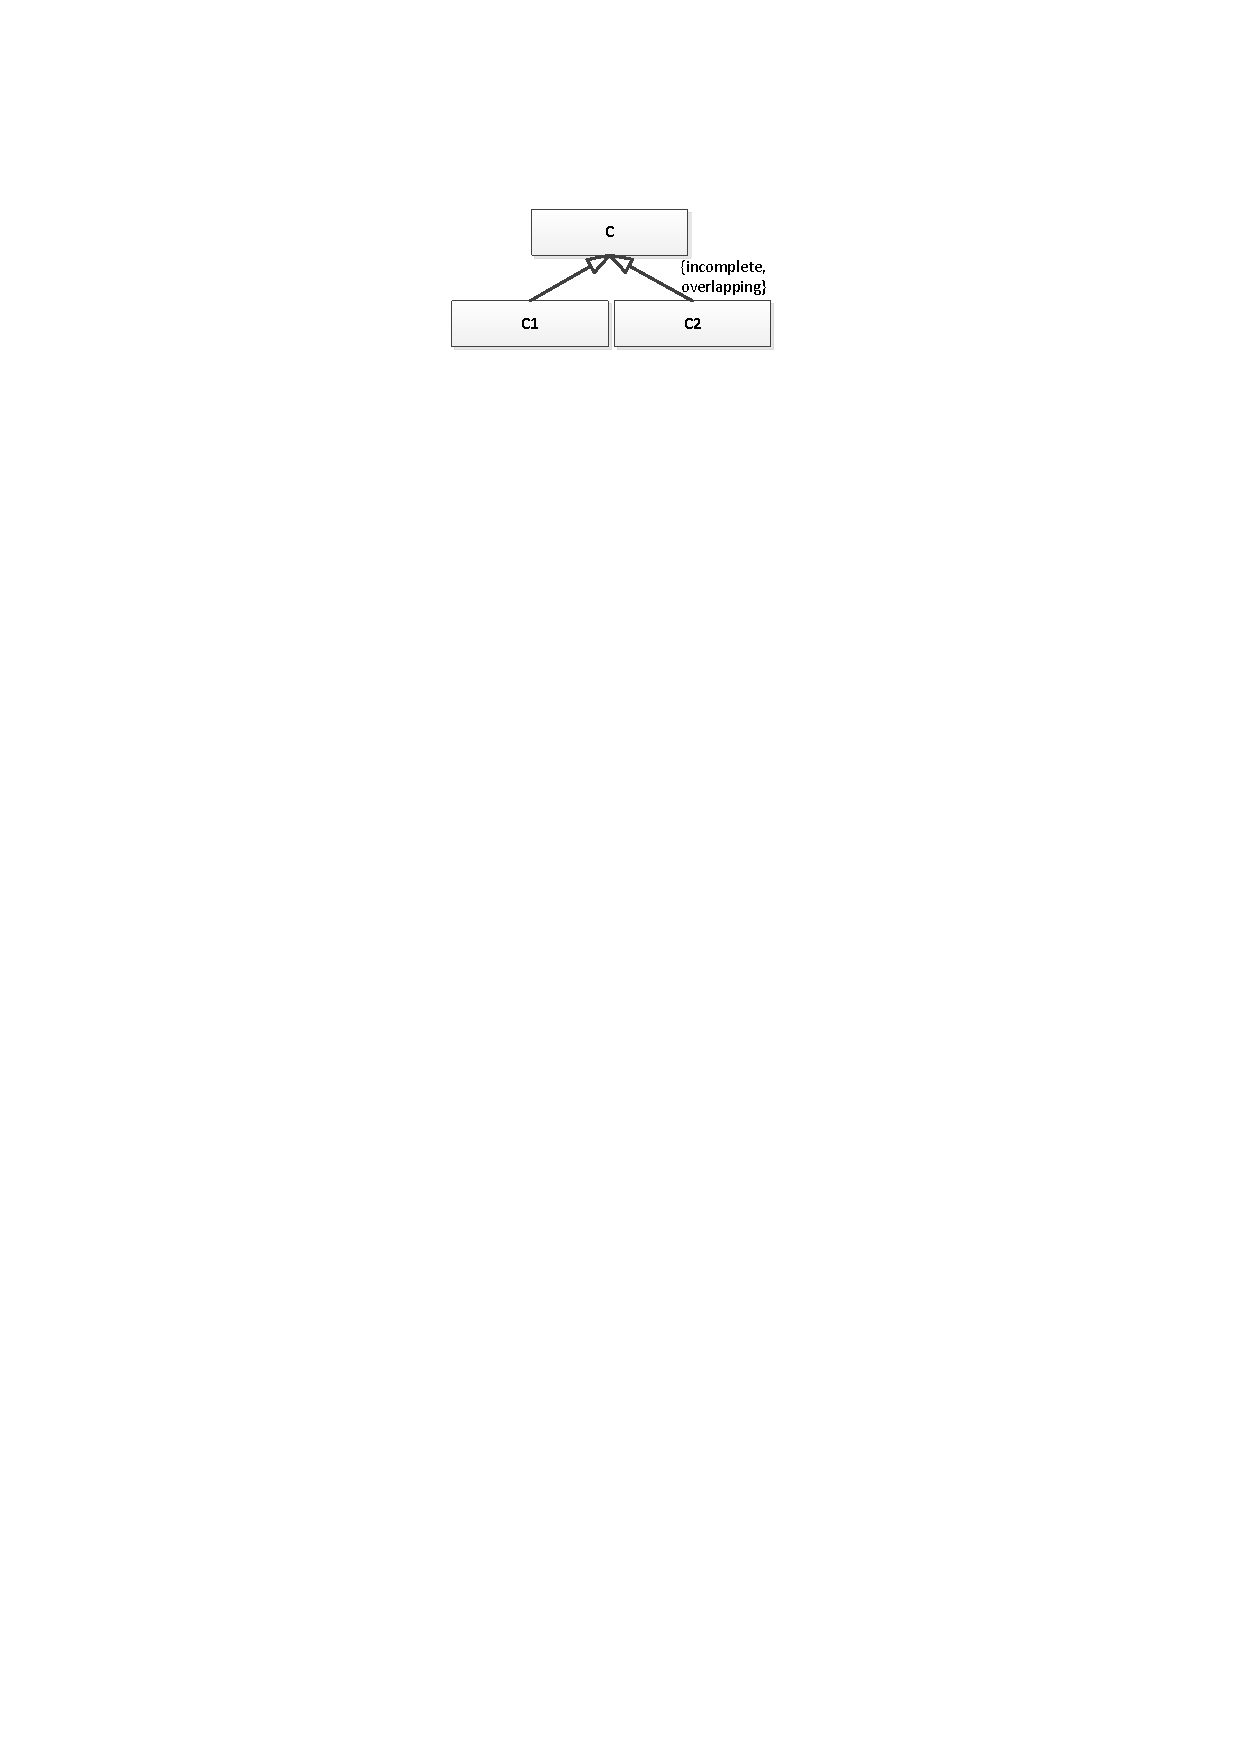
\includegraphics[trim = 76mm 235mm 72mm 25mm, clip, scale=0.75]{./diagrams/chapter5/IncompleteOverlapping}
      Class \texttt{C} is specialized by the overlapping classes \texttt{C1} and \texttt{C2} which do not cover class \texttt{C}  
     \vspace{2mm}
    \end{minipage}
    &
    \begin{minipage}{\dltablespacing}
       $\begin{aligned}   
	  &C_1 \sqsubseteq C  \\  
	  &C_2 \sqsubseteq C 
       \end{aligned}$     
    \end{minipage}
    &
      $\begin{aligned}
	  &\texttt{Class: C}\\[\owlspacing]
          &\texttt{Class: C1}\\[\owlspacing]
	  &\texttt{\hspace*{0.20cm} SubClassOf: C}\\[\owlspacing]
          &\texttt{Class: C2}\\[\owlspacing]
          &\texttt{\hspace*{0.20cm} SubClassOf: C}	
     \end{aligned}$
    &
    \ref{sec_Generalization/Specialization of Classes} \linebreak p. \pageref{sec_Generalization/Specialization of Classes}\\
     \hline       
    \begin{minipage}{\umltablespacing}
    %trim option's parameter order: left bottom right top
      \centering\hspace*{-4.7mm}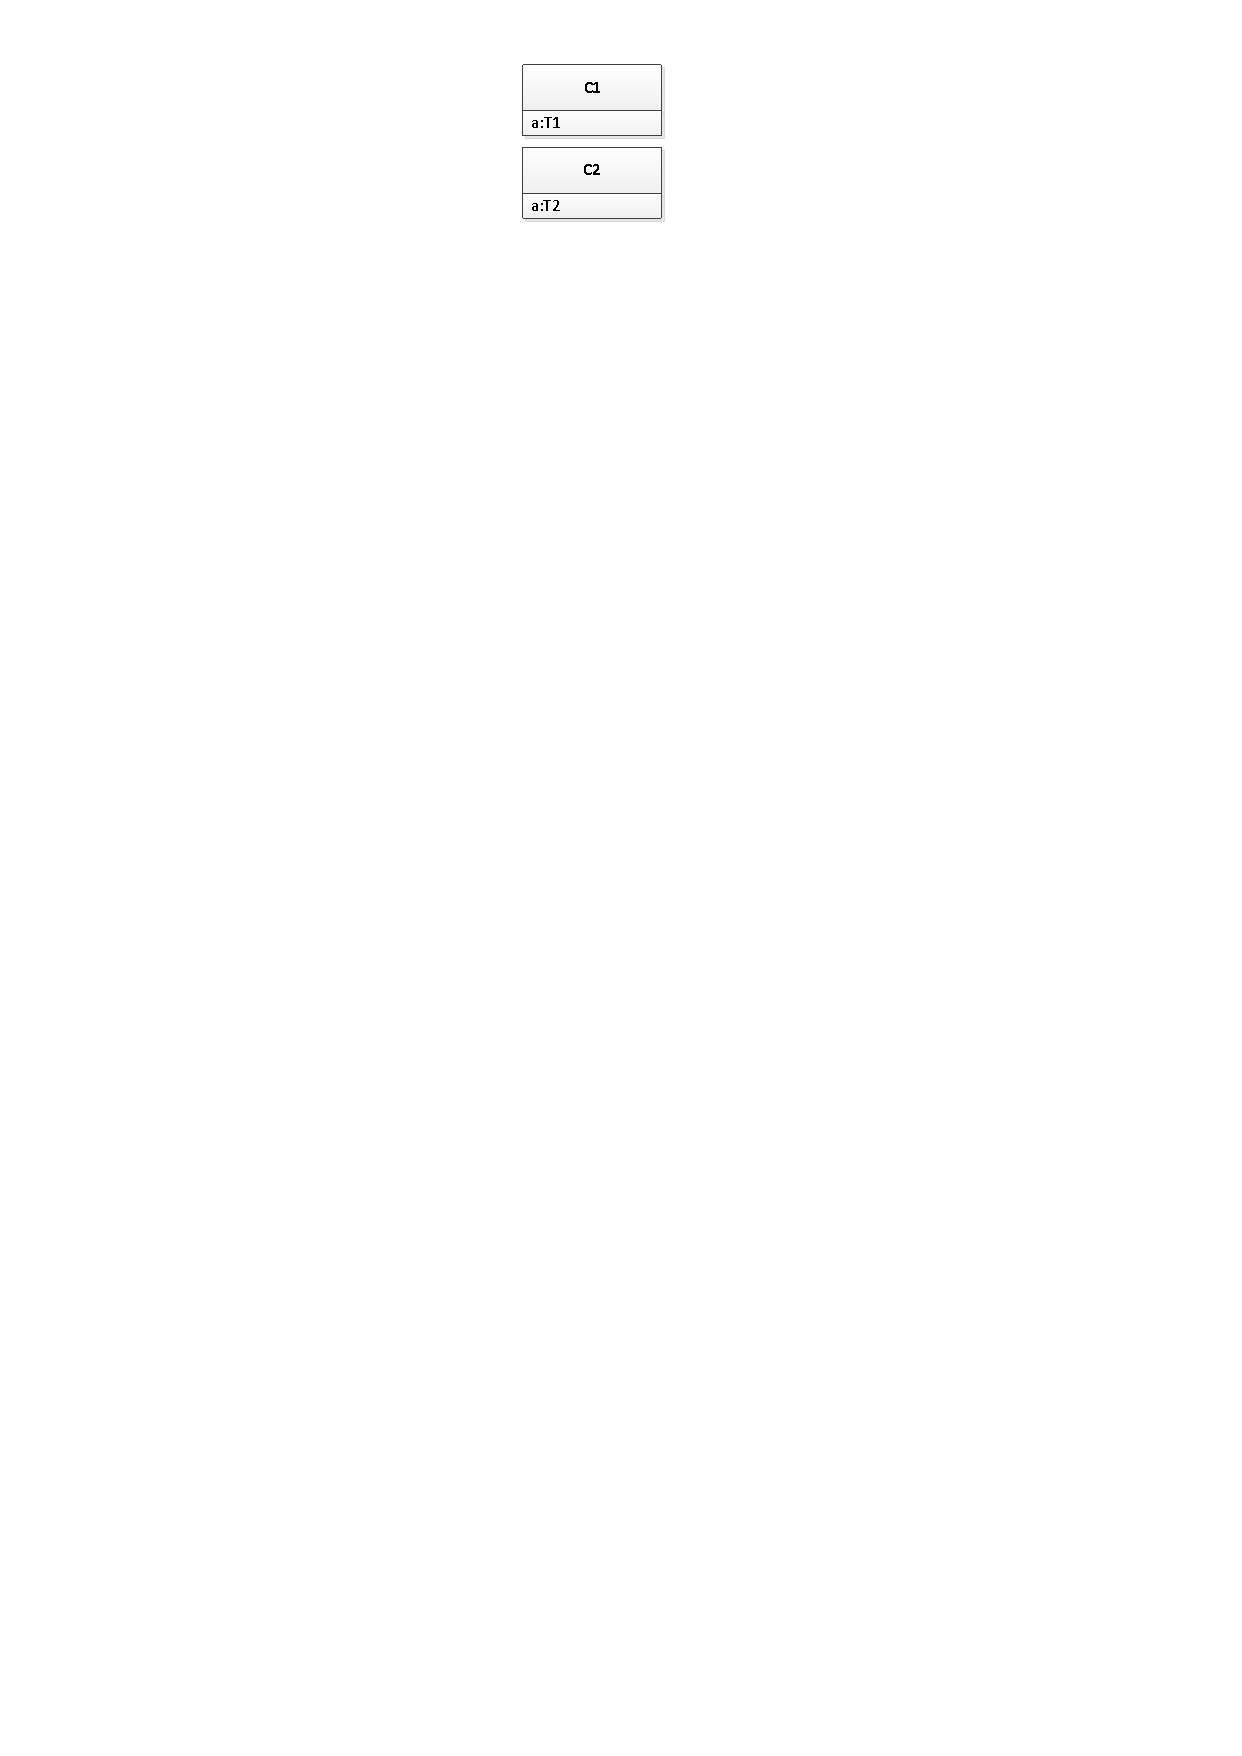
\includegraphics[trim = 76mm 255mm 72mm 0mm, clip, scale=0.75]{./diagrams/chapter5/QualifiedAttributeNamesSmall}
      Classes \texttt{C1} and \texttt{C2} both have an attribute \texttt{a} respectively of type \texttt{T1} and \texttt{T2}.
     \vspace{2mm}
    \end{minipage}
    &
    \begin{minipage}{\dltablespacing}
    $\begin{aligned}
  	&\exists a.\top \sqsubseteq C_1 \sqcup C_2\\
  	&\exists a^-.\top \sqsubseteq T_1 \sqcup T_2\\
  	&C_1 \sqsubseteq \exists a.\top \sqcap (\leq 1 \hspace*{2pt} a. \top)\\
  	&C_2 \sqsubseteq \exists a.\top \sqcap (\leq 1 \hspace*{2pt} a. \top)
    \end{aligned}$
    \end{minipage}
    &
     $\begin{aligned} 
	&\texttt{Class: C1} \\[\owlspacing]
   	&\texttt{\hspace*{2mm}SubClassOf:}\\[\owlspacing]
   	&\texttt{\hspace*{4mm}t exactly 1 Thing}\\[\owlspacing]	
	&\texttt{Class: C2} \\[\owlspacing]
   	&\texttt{\hspace*{2mm}SubClassOf:}\\[\owlspacing]
   	&\texttt{\hspace*{4mm}t exactly 1 Thing}\\[\owlspacing]	
	&\texttt{Class: T1} \\[\owlspacing]
	&\texttt{Class: T2} \\[\owlspacing]	
	&\texttt{ObjectProperty: a} \\[\owlspacing]
	&\texttt{\hspace*{2mm} Domain: C1 or C2} \\[\owlspacing]
	&\texttt{\hspace*{2mm} Range: T1 or T2} \\
    \end{aligned}$     
    &
    \ref{sec_Multiplicity_Attribute} \linebreak p. \pageref{sec_Multiplicity_Attribute} \linebreak and \linebreak \ref{sec_attributes_sroiq} \linebreak p. \pageref{sec_attributes_sroiq}
    \linebreak and \linebreak
    \ref{subsec_Attributes and Associations} \linebreak p. \pageref{subsec_Attributes and Associations} \\
     \hline 
    \begin{minipage}{\umltablespacing}
    %trim option's parameter order: left bottom right top
      \centering\hspace*{-4.5mm}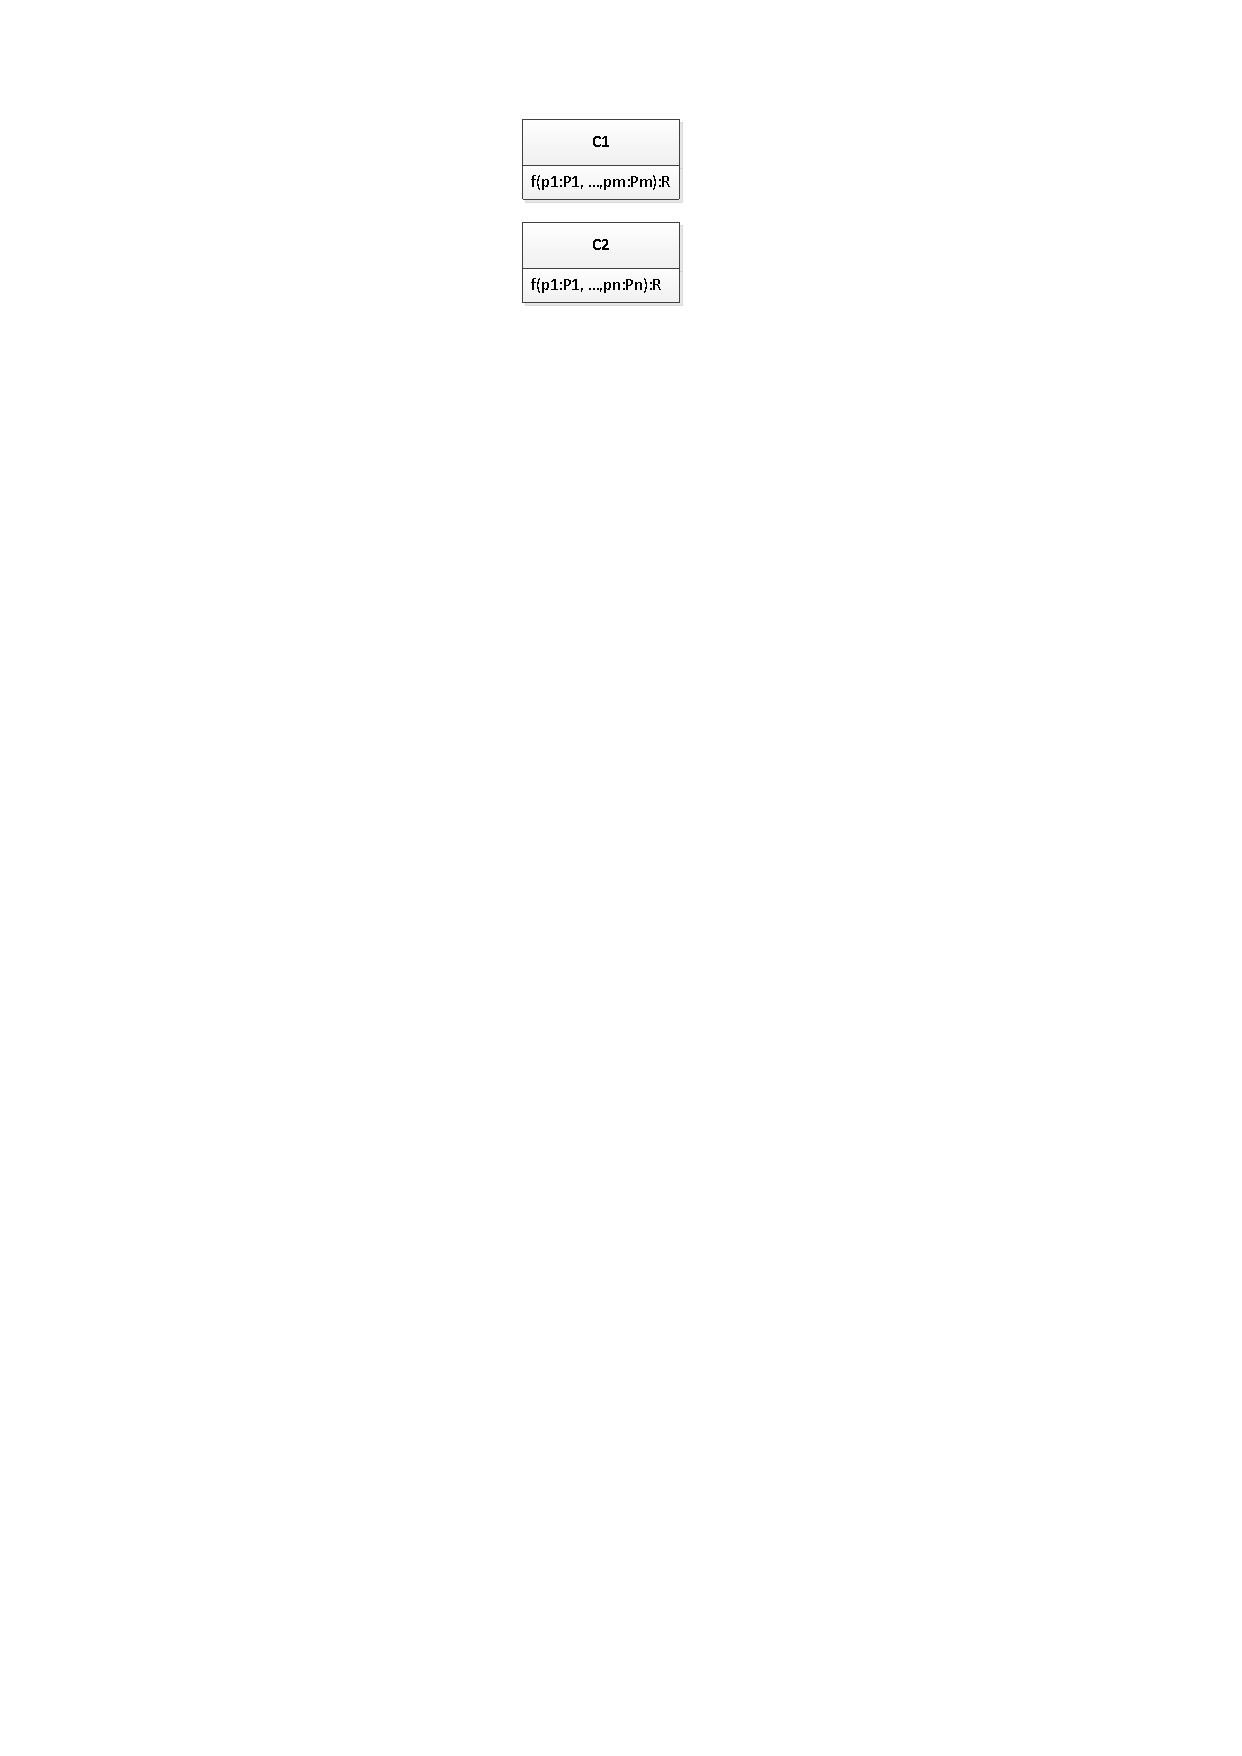
\includegraphics[trim = 76mm 235mm 72mm 10mm, clip, scale=0.75]{./diagrams/chapter5/QualifiedOperationNamesSmall}
      Classes \texttt{C1} and \texttt{C2} both have an operation \texttt{f} with return value \texttt{R} and respective parameters \linebreak \texttt{p1:P1, ..., pm:Pm} and \linebreak
      \texttt{p1:P1, ..., pn:Pn} with \texttt{m}<\texttt{n}.
     \vspace{2mm}
    \end{minipage}
    &
      \begin{minipage}{\dltablespacing}
      $\begin{aligned}
      \\
  	&C_{1_{f(P_1, \ldots, P_m):R}} \sqsubseteq\\
  	\hspace*{1mm}& \exists f^-.\top \sqcap (\leq 1 f^-.\top) \hspace*{1mm} \sqcap \\
  	 \hspace*{1mm}& \exists p_1.\top \sqcap (\leq 1 p_1.\top) \hspace*{1mm} \sqcap \\
  	\hspace*{1mm}& \vdots  \\
  	\hspace*{1mm}& \exists p_m.\top \sqcap (\leq 1 p_m.\top) \hspace*{1mm} \sqcap \\
  	\hspace*{1mm}& \exists r_R.\top \sqcap (\leq 1 r_R.\top)\\
	&C_1 \sqsubseteq \exists f. C_{1_{f(P_1, \ldots, P_m):R}}\\
	\\
  	&C_{2_{f(P_1, \ldots, P_n):R}} \sqsubseteq\\
  	\hspace*{1mm}& \exists f^-.\top \sqcap (\leq 1 f^-.\top) \hspace*{1mm} \sqcap \\
  	 \hspace*{1mm}& \exists p_1.\top \sqcap (\leq 1 p_1.\top) \hspace*{1mm} \sqcap \\
  	\hspace*{1mm}& \vdots  \\
  	\hspace*{1mm}& \exists p_n.\top \sqcap (\leq 1 p_n.\top) \hspace*{1mm} \sqcap \\
  	\hspace*{1mm}& \exists r_R.\top \sqcap (\leq 1 r_R.\top)\\
	&C_2 \sqsubseteq \exists f. C_{2_{f(P_1, \ldots, P_n):R}}\\
	\\
    	&\exists p_i.\top \sqsubseteq C_{1_{f(P_1, \ldots, P_m):R}} \\
    	&\sqcup C_{2_{f(P_1, \ldots, P_n):R}}\\   
    	&\exists p_i^-.\top \sqsubseteq P_i \hspace*{5mm} i = 1, \ldots, m \\
    	\\
    	&\exists p_j.\top \sqsubseteq C_{2_{f(P_1, \ldots, P_n):R}} \\
    	&\exists p_j^-.\top \sqsubseteq P_j \hspace*{5mm} j = m+1, \ldots, n \\
    	\\
  	&\exists f^-.\top \sqsubseteq C_{1_{f(P_1, \ldots, P_m):R}} \\
  	&\sqcup C_{2_{f(P_1, \ldots, P_n):R}}   \\
  	&\exists f.\top \sqsubseteq C_1 \sqcup C_2 \\
  	\\
  	&\exists r_R.\top \sqsubseteq C_{1_{f(P_1, \ldots, P_m):R}} \\
  	&\sqcup C_{2_{f(P_1, \ldots, P_n):R}}\\
	&\exists r_R^-.\top \sqsubseteq R\\
	\\
     \end{aligned}$
     Note that determinism of the return values is not enforced.\linebreak 
      \end{minipage}
    &
      $\begin{aligned} 
	&\texttt{Class: P1} \\[\owlspacing]
	&\texttt{\hspace*{6mm}} \vdots \\[\owlspacing]
	&\texttt{Class: Pn} \\[\owlspacing]
	&\texttt{Class: R} \\[\owlspacing]
  	&\texttt{Class: C1\_f(P1,..., Pm)\_R} \\[\owlspacing]
  	&\texttt{\hspace*{2mm}SubClassOf:}\\[\owlspacing]
  	&\texttt{\hspace*{4mm}f\_inv exactly 1 Thing}\\[\owlspacing]
  	&\texttt{\hspace*{6mm}and}\\[\owlspacing]
  	&\texttt{\hspace*{4mm}p1 exactly 1 Thing and}\\[\owlspacing]
  	&\texttt{\hspace*{6mm}} \vdots \\[\owlspacing]
  	&\texttt{\hspace*{4mm}pm exactly 1 Thing and}\\[\owlspacing]
  	&\texttt{\hspace*{4mm}r\_R exactly 1 Thing}\\[\owlspacing]
         &\texttt{\hspace*{2mm}Haskey:}\\[\owlspacing] 
         &\texttt{\hspace*{4mm}f\_inv, p1, ..., pm}\\[\owlspacing]   	
         &\texttt{Class: C1}\\[\owlspacing]
         &\texttt{\hspace*{2mm}SubClassOf: }\\[\owlspacing]
         &\texttt{\hspace*{4mm}f some C1\_f(P1,..., Pm)\_R}\\    
%          \\
  	&\texttt{Class: C2\_f(P1,..., Pn)\_R} \\[\owlspacing]
  	&\texttt{\hspace*{2mm}SubClassOf:}\\[\owlspacing]
  	&\texttt{\hspace*{4mm}f\_inv exactly 1 Thing}\\[\owlspacing]
  	&\texttt{\hspace*{6mm}and}\\[\owlspacing]
  	&\texttt{\hspace*{4mm}p1 exactly 1 Thing and}\\[\owlspacing]
  	&\texttt{\hspace*{6mm}} \vdots \\[\owlspacing]
  	&\texttt{\hspace*{4mm}pn exactly 1 Thing and}\\[\owlspacing]
  	&\texttt{\hspace*{4mm}r\_R exactly 1 Thing}\\[\owlspacing]
         &\texttt{\hspace*{2mm}Haskey:}\\[\owlspacing] 
         &\texttt{\hspace*{4mm}f\_inv, p1, ..., pn} \\[\owlspacing]  	
         &\texttt{Class: C2}\\[\owlspacing]
         &\texttt{\hspace*{2mm}SubClassOf: }\\[\owlspacing]
         &\texttt{\hspace*{4mm}f some C2\_f(P1,..., Pm)\_R}\\           
%          \\
          &\texttt{ObjectProperty: p1}\\[\owlspacing]
          &\texttt{\hspace*{2mm} Domain: C1\_f(P1, ..., Pm)\_R} \\[\owlspacing] 
          &\texttt{\hspace*{4mm} or C2\_f(P1, ..., Pn)\_R}\\[\owlspacing]
          &\texttt{\hspace*{2mm} Range: P1}\\[\owlspacing]
          &\texttt{\hspace*{4mm}}\vdots \\[\owlspacing]
          &\texttt{ObjectProperty: pm}\\[\owlspacing]
          &\texttt{\hspace*{2mm} Domain: C1\_f(P1, ..., Pm)\_R} \\[\owlspacing]
          &\texttt{\hspace*{4mm} or C2\_f(P1, ..., Pn)\_R}\\[\owlspacing]
          &\texttt{\hspace*{2mm} Range: Pm}\\[\owlspacing]
          &\texttt{ObjectProperty: pk}\\[\owlspacing]
          &\texttt{\hspace*{2mm} Domain: C2\_f(P1, ..., Pn)\_R}\\[\owlspacing]
          &\texttt{\hspace*{2mm} Range: Pk}\\[\owlspacing]
          &\texttt{\hspace*{4mm}}\vdots \\[\owlspacing]
          &\texttt{ObjectProperty: pn}\\[\owlspacing]
          &\texttt{\hspace*{2mm} C2\_f(P1, ..., Pn)\_R}\\[\owlspacing]
          &\texttt{\hspace*{2mm} Range: Pn} \\[\owlspacing]       
%  \\
          &\texttt{ObjectProperty: f\_inv}\\[\owlspacing]
          &\texttt{\hspace*{2mm} Domain: C1\_f(P1, ..., Pm)\_R} \\[\owlspacing]
          &\texttt{\hspace*{4mm} or C2\_f(P1, ..., Pn)\_R}\\[\owlspacing]
          &\texttt{\hspace*{2mm} Range: C1 or C2}\\[\owlspacing]
          &\texttt{ObjectProperty: f}\\[\owlspacing]
          &\texttt{\hspace*{2mm} InverseOf: f\_inv}\\[\owlspacing]  
          &\texttt{ObjectProperty: r\_R}\\[\owlspacing]
          &\texttt{\hspace*{2mm} Domain: C1\_f(P1, ..., Pm)\_R} \\[\owlspacing]
          &\texttt{\hspace*{4mm} or C2\_f(P1, ..., Pn)\_R}\\[\owlspacing]
          &\texttt{\hspace*{2mm} Range: R}\\
     \end{aligned}$   
    &
    \ref{sec_operations_sroiq} \linebreak p. \pageref{sec_operations_sroiq} \linebreak and \ref{sec_Operations Revisited} \linebreak p. \pageref{sec_Operations Revisited}
    \linebreak and \linebreak
    \ref{subsec_Operations and Parameters} \linebreak p. \pageref{subsec_Operations and Parameters}\\
     \hline     
    \end{longtable} 


   %\textbf{Todo:} Add examples of the same attributes and operations on two different classes